% =====================================================================
% arXiv preprint version.
% Standard article class (single column, 11pt) for broad TeX compatibility on arXiv.
% Content identical to the Neurophotonics submission version; SPIE-specific class,
% ORCID, and journal typesetting removed. Recommended arXiv category: physics.med-ph
% (primary), cross-list physics.optics and q-bio.NC.
% =====================================================================
\documentclass[11pt]{article}

\usepackage[margin=1in]{geometry}
\usepackage{amsmath,amssymb}
\usepackage{graphicx}
\usepackage{booktabs}
\usepackage{multirow}
\usepackage{array}
\usepackage{enumitem}
\usepackage{microtype}
\usepackage[hidelinks]{hyperref}
\usepackage{authblk}
\emergencystretch=3em

\renewcommand\Authfont{\bfseries}
\setlength{\affilsep}{0.5em}

\title{\textbf{Partial-volume correction in continuous-wave fNIRS: operating regime, a Monte-Carlo convergence caveat, and a reproducible pipeline}}

\author[1]{Neth Sagara}
\author[1]{Amir Ahsan\thanks{Corresponding author: \texttt{aahsan@ivc.edu}}}
\affil[1]{Department of Physics, Irvine Valley College, Irvine, CA 92618, USA}

\date{}

\begin{document}
\maketitle

% ---------------------------------------------------------------------
% Structured abstract (Neurophotonics format)
% ---------------------------------------------------------------------
\begin{abstract}
\noindent Functional near-infrared spectroscopy (fNIRS) is widely used in cognitive and clinical neuroscience, but routine Modified Beer--Lambert Law (MBLL) processing treats the head as homogeneous and underestimates cortical hemoglobin changes by roughly an order of magnitude. We present a transparent, reproducible partial-volume correction and, more importantly, two methodological cautions that apply to any correction of this kind. The correction decomposes MBLL bias into a differential-pathlength factor and a partial-volume factor $\kappa_{\mathrm{PV}}=1/f_{\mathrm{cortex}}$ applied at the optical-density level, with a short-separation-regression (SSR) term $\kappa_{\mathrm{SSR}}$ reported as a diagnostic rather than applied. Cortical sensitivity fractions $f_{\mathrm{cortex}}$ come from a converged two-layer Monte Carlo, cross-checked against a finite-difference solver and published atlas Monte Carlo, and the pipeline is tested on synthetic data with known ground truth (five subjects, source--detector separations 25--40\,mm) and on the five-subject BIDS-NIRS-Tapping dataset. Three findings result. First, the analytical Kienle Jacobian, evaluated by a fixed-point (fixed-grid) Hankel quadrature, is not converged for $f_{\mathrm{cortex}}$ and overstates it by about an order of magnitude (this is a property of that quadrature, not of the Kienle model itself); the converged fraction is small (0.04--0.11), so $\kappa_{\mathrm{PV}}$ is large (9--23). Second, because the diluted cortical signal falls below the shot-noise floor at short separations, the correction is reliable only at long separations ($\geq$38\,mm), where it reduces HbO$_2$ root-mean-square error by 44--45\%, and is harmful at 25\,mm. Third, the short-separation-regression $R^2$ is a variance-removal diagnostic, not an amplitude factor: $1/(1-R^2_{\mathrm{SS}})$ is an inverse residual-\emph{variance} ratio (the amplitude ratio would be $\sqrt{1-R^2_{\mathrm{SS}}}$) and $R^2$ alone cannot identify cortical loss, so it is reported, not applied. Applied in vivo with a per-channel, contralateral, quality-controlled, fixed-window analysis, the correction recovers a physiologically plausible group-mean cortical $\Delta[\mathrm{HbO}_2]$ of $0.84\pm0.31\,\mu$M ($\sim$7$\times$ the uncorrected estimate). This single-dataset result is a demonstration, not a validation of accuracy.
\end{abstract}

\vspace{0.5em}\noindent\textbf{Keywords:} functional near-infrared spectroscopy, partial volume effect, short-separation regression, Modified Beer-Lambert law, cortical sensitivity, quantitative neuroimaging
\vspace{0.5em}

% ---------------------------------------------------------------------
% Body content (sections 1 through Conclusions)
% ---------------------------------------------------------------------
\section{Introduction}

\subsection{Clinical context and motivation}

\noindent Functional near-infrared spectroscopy (fNIRS) monitors cortical hemodynamics non-invasively by transmitting near-infrared light (650-950\,nm) through the scalp and measuring intensity changes at one or more detector positions\cite{r1,r2,r3}. Since J\"obsis\cite{r41} first demonstrated transcranial optical monitoring, the technique has become widely used in cognitive neuroscience and clinical research owing to its portability, tolerance of motion, and ability to resolve both oxygenated (HbO$_2$) and deoxygenated (HbR) hemoglobin.

The clinical promise of fNIRS is substantial. It has been deployed for bedside monitoring of neonatal cerebral oxygenation\cite{r4}, intraoperative surveillance during cardiac surgery\cite{r5}, stroke rehabilitation assessment\cite{r6}, and brain-computer interfaces for communication and motor restoration\cite{r7}. In each of these settings, the ability to obtain \textit{quantitative} hemoglobin concentration estimates, rather than merely qualitative trends, is critical for establishing diagnostic thresholds, comparing across subjects, tracking longitudinal change and informing clinical decisions\cite{r8}.

However, fNIRS measurements are not inherently quantitative. The standard signal-processing step converts optical density changes to concentration changes via the Modified Beer-Lambert Law (MBLL)\cite{r9}, which treats the interrogated tissue as optically homogeneous. This assumption is fundamentally violated when photons traverse scalp, skull, cerebrospinal fluid and cortex, layers whose absorption and scattering coefficients differ by factors of two or more\cite{r10,r11,r12}. The resulting systematic underestimation of cortical hemoglobin changes, typically by a factor of 3-10$\times$, has long been recognized as a barrier to the technique's clinical translation\cite{r13}.

\subsection{The quantification gap}

Despite decades of fNIRS development, much of the clinical and neuroscience literature reports results in arbitrary units or qualitative terms, limiting cross-study comparison and meta-analysis\cite{r2}. Three distinct mechanisms contribute to the quantification gap.

\textit{Differential pathlength error.} The DPF assumed in processing is typically a population-average value. Monte Carlo simulations and time-resolved measurements show that the true effective DPF can differ by 10-30\% depending on tissue geometry, wavelength and subject age\cite{r12,r14}.

\textit{Partial volume effect.} MBLL presupposes uniform absorption changes throughout the sampled volume. Hemodynamic changes are localized in the cortex, which (according to converged Monte Carlo light transport, both for a two-layer slab and for realistic head models\cite{r10,r12}) contributes only $\sim$4\% of the total channel sensitivity at 25\,mm rising to $\sim$11\% at 40\,mm for the converged two-layer model ($\sim$13\% for the Colin27 atlas Monte Carlo\cite{r10}; Section~\ref{sec:atlas_compare}). The resulting severe dilution systematically underestimates cortical concentrations by roughly a factor of nine to twenty-three when using single-layer approximations.

\textit{Superficial signal contamination.} Cardiac pulsation ($\sim$1\,Hz), respiration ($\sim$0.25\,Hz) and Mayer waves ($\sim$0.1\,Hz) in extracerebral tissue modulate the measured intensity and introduce both bias and variance\cite{r15,r16,r17}.

Short-separation regression (SSR) addresses the third source of bias by using a detector at small source-detector separation (SDS $<$ 15\,mm) as a reference for the superficial signal\cite{r18,r19}. However, SSR alone does not correct for partial volume effects, which typically cause MBLL to underestimate true cortical concentrations by a factor of 3-10$\times$ depending on SDS\cite{r10,r13}. Existing approaches to the partial volume problem include image reconstruction methods\cite{r13}, atlas-based sensitivity weighting\cite{r10} and Monte Carlo simulation of light transport in anatomically realistic head models\cite{r12,r20}. While effective, these methods either require anatomical imaging data, demand substantial computational resources, or lack a transparent, analytically tractable structure.

\subsection{Contribution of this work}

The multiplicative correction we use is deliberately not new. The partial-volume factor $\kappa_{\mathrm{PV}}=1/f_{\mathrm{cortex}}$ is exactly the sensitivity-weighting that underlies atlas-based partial-volume corrections\cite{r10,r13}, short-separation regression (SSR) is standard\cite{r18,r19}, and the differential-pathlength factor $\kappa_{\mathrm{DPF}}$ is textbook. Our contribution is instead \emph{two methodological cautions} that apply to any correction of this form, made concrete and reproducible by assembling the factors into a single transparent pipeline: a numerical caution about how $f_{\mathrm{cortex}}$ must be computed, and a statistical caution about how the SSR term must be treated. A practical operating-regime result follows from the first. We state all three explicitly.

\begin{enumerate}
\item \emph{A numerical caution (novel).} Cortical sensitivity fractions must be computed from a converged forward model. We show that the same quantity computed from the analytical Kienle Jacobian by zeroth-order Hankel transform is \emph{not} quadrature-converged and overestimates $f_{\mathrm{cortex}}$ by roughly an order of magnitude at default settings (Section~\ref{sec:hankel_instab}), which makes the partial-volume factor appear near unity and would silently defeat the correction. We therefore calibrate $f_{\mathrm{cortex}}$ against a converged Monte Carlo.
\item \emph{A statistical clarification (novel).} The common SSR-restoration factor $1/(1-R^2_{\mathrm{SS}})$ is an inverse residual-\emph{variance} ratio, not an amplitude-restoration factor (the corresponding amplitude ratio is $\sqrt{1-R^2_{\mathrm{SS}}}$), and $R^2_{\mathrm{SS}}$ pools superficial variance, cortical--systemic covariance, measurement noise, and short-channel cortical sensitivity into one number, so it cannot identify cortical loss. It should be reported as a variance-removal diagnostic, not applied; applying it in vivo would inflate the recovered amplitude roughly twofold.
\item \emph{An operating regime (consequence of the first).} Because the converged $f_{\mathrm{cortex}}$ is small, the partial-volume factor is large ($\kappa_{\mathrm{PV}}\approx9$--$23$); at short separations the diluted cortical signal falls below the measurement-noise floor, so the correction amplifies noise and is harmful. The method is reliable only at long separations ($\geq$\,38\,mm).
\end{enumerate}

We characterize the correction on synthetic data with known ground truth across SDS from 25 to 40\,mm, cross-validate the forward model against a finite-difference solver and atlas Monte Carlo, analyze sensitivity to tissue-model assumptions and the cerebrospinal-fluid layer, and apply the pipeline end-to-end to a publicly available finger-tapping dataset. A note on the forward model up front: we use a two-layer slab as a \emph{controlled testbed} for the synthetic validation, because it isolates the algebraic behaviour of the correction under exactly known conditions; for real heads we add the cerebrospinal-fluid layer, and we recommend a CSF-augmented (three-layer or richer) model in practice (Section~\ref{sec:mismatch_results}). We are explicit about scope: the in-vivo result is a proof-of-concept on a single five-subject dataset \emph{without} concurrent ground truth, so it demonstrates physiological plausibility rather than measured accuracy. All code, a pedagogical guide, and a runnable notebook are provided for full reproducibility.

\section{Theory}

\subsection{Modified Beer-Lambert Law}

For a dual-wavelength continuous-wave fNIRS system, MBLL relates the change in optical density $\Delta\mathrm{OD}(\lambda)$ to chromophore concentration changes\cite{r9,r21}:
\begin{equation}
\Delta\mathrm{OD}(\lambda) = \ln(10)\,\bigl[\varepsilon_{\mathrm{HbO_2}}(\lambda)\,\Delta C_{\mathrm{HbO_2}} + \varepsilon_{\mathrm{HbR}}(\lambda)\,\Delta C_{\mathrm{HbR}}\bigr] \cdot L \cdot \mathrm{DPF}(\lambda)
\label{eq:mbll}
\end{equation}
where $\varepsilon$ denotes the decadic (base-10) molar extinction coefficient (mM$^{-1}$\,cm$^{-1}$; tabulated values from Prahl\cite{r23}), $L$ is the source-detector separation, and DPF is the differential pathlength factor accounting for scattering-induced path elongation. Tabulated extinction coefficients from the Prahl/Oregon Medical Laser Center compilation are conventionally reported in the decadic (base-10) convention, while the absorption coefficient $\mu_a$ used in diffusion models is defined in the Napierian (base-$e$) convention: $\mu_a = \varepsilon \ln(10)\,C$, where $\ln(10) \approx 2.3026$. The factor of $\ln(10)$ in equation~(\ref{eq:mbll}) converts between these conventions so that $\Delta\mathrm{OD}$ is expressed in Napierian units consistent with the diffusion-theory absorption coefficients used throughout this work. This explicit conversion ensures compatibility with standard spectroscopic databases and facilitates direct comparison with experimental fNIRS data. DPF values of 5-7 are typical for adult head measurements and vary with wavelength and age\cite{r14,r22}. Because scattering and absorption are wavelength-dependent, DPF differs at each measurement wavelength. The two-wavelength system must therefore normalize each wavelength by its own pathlength. Defining $\ell(\lambda) = \ln(10) \cdot L \cdot \mathrm{DPF}(\lambda)$, the system reads
\begin{equation}
\begin{bmatrix} \Delta\mathrm{OD}(\lambda_1)/\ell(\lambda_1) \\ \Delta\mathrm{OD}(\lambda_2)/\ell(\lambda_2) \end{bmatrix}
= \begin{bmatrix} \varepsilon_{\mathrm{HbO_2}}(\lambda_1) & \varepsilon_{\mathrm{HbR}}(\lambda_1) \\
\varepsilon_{\mathrm{HbO_2}}(\lambda_2) & \varepsilon_{\mathrm{HbR}}(\lambda_2) \end{bmatrix}
\begin{bmatrix} \Delta C_{\mathrm{HbO_2}} \\ \Delta C_{\mathrm{HbR}} \end{bmatrix}
\label{eq:mbll_matrix}
\end{equation}
and is solved by pseudoinversion of the extinction coefficient matrix. If a single scalar DPF is used for both wavelengths, as is common in many fNIRS processing pipelines, a wavelength-dependent bias is introduced whose magnitude depends on the ratio of the true DPFs at the two wavelengths.

Table~\ref{tab:extinction} lists the decadic molar extinction coefficients used in this study at the 10 wavelengths supported by our implementation, including the two wavelengths (760 and 850\,nm) employed in the simulations. These values were obtained from the Prahl/Oregon Medical Laser Center tabulation\cite{r23}, originally reported in cm$^{-1}$\,M$^{-1}$ and converted to mM$^{-1}$\,cm$^{-1}$ by dividing by 1000.

\begin{table}[ht]
\centering
\caption{Decadic (base-10) molar extinction coefficients for HbO$_2$ and HbR at selected fNIRS wavelengths\cite{r23}. Units: mM$^{-1}$\,cm$^{-1}$.}
\label{tab:extinction}
\begin{tabular}{@{}ccc@{}}
\toprule
\textbf{Wavelength (nm)} & $\varepsilon_{\mathrm{HbO_2}}$ & $\varepsilon_{\mathrm{HbR}}$ \\
\midrule
690 & 0.276 & 2.052 \\
700 & 0.290 & 1.794 \\
730 & 0.390 & 1.102 \\
750 & 0.518 & 1.405 \\
760 & 0.586 & 1.549 \\
780 & 0.710 & 1.075 \\
800 & 0.816 & 0.762 \\
830 & 0.974 & 0.693 \\
850 & 1.058 & 0.691 \\
880 & 1.154 & 0.726 \\
\bottomrule
\end{tabular}
\end{table}

\subsection{The $\kappa$ correction framework}

\subsubsection{Origin of the bias: MBLL in layered media.}

To motivate the correction framework, consider what MBLL actually estimates when applied to a two-layer medium. The measured optical density change at a long-separation channel contains weighted contributions from both layers:
\begin{equation}
\Delta\mathrm{OD}_{\mathrm{measured}} = f_{\mathrm{cortex}} \cdot \Delta\mathrm{OD}_{\mathrm{cortex}} + (1 - f_{\mathrm{cortex}}) \cdot \Delta\mathrm{OD}_{\mathrm{superficial}}
\label{eq:od_layers}
\end{equation}
where $f_{\mathrm{cortex}}$ is the cortical sensitivity fraction defined in section~\ref{sec:jacobian}. Because MBLL assumes homogeneous tissue, its estimate of the concentration change is
\begin{equation}
\Delta C_{\mathrm{MBLL}} = \frac{\Delta\mathrm{OD}_{\mathrm{measured}}}{\ln(10)\,\varepsilon \cdot L \cdot \mathrm{DPF}}
\label{eq:mbll_bias_origin}
\end{equation}
which is a weighted average of all layers, not the true cortical concentration. Since only the cortical layer exhibits task-evoked hemodynamic changes, the MBLL estimate is systematically attenuated by a factor proportional to $f_{\mathrm{cortex}}$ and contaminated by superficial physiology. Recovering the true cortical concentration requires inverting these effects.

\subsubsection{Multiplicative correction structure.}

The relationship between the uncorrected and corrected concentration estimates can be expressed as a multiplicative correction:
\begin{equation}
\Delta C_{\mathrm{corrected}} = \kappa \times \Delta C_{\mathrm{MBLL}}
\label{eq:correction}
\end{equation}
where $\Delta C_{\mathrm{MBLL}}$ is the na\"ive MBLL estimate from uncorrected optical density. In practice, the individual corrections (SSR, PV scaling) are applied at the OD level before MBLL inversion (see Section~\ref{sec:pipeline}); Equation~\eqref{eq:correction} describes the net effect of all corrections in concentration space rather than the implementation order. The \emph{applied} correction factor decomposes into two physically independent components; the short-separation-regression attenuation $\kappa_{\mathrm{SSR}}(\lambda)$ is computed per wavelength and reported as a diagnostic (Section~\ref{sec:kappa_ssr_diag}) rather than applied:
\begin{equation}
\kappa_{\mathrm{applied}} = \kappa_{\mathrm{DPF}} \times \kappa_{\mathrm{PV}}
\label{eq:kappa}
\end{equation}

Equation~(\ref{eq:kappa}) is written in scalar form for interpretability, but it is a \emph{descriptive summary}. Because $f_{\mathrm{cortex}}$, DPF and the extinction coefficients are all wavelength-dependent, the exact dual-wavelength operation is wavelength-diagonal and matrix-valued, applied at the optical-density level before spectroscopic inversion:
\begin{equation}
\widehat{\mathbf{c}} = \mathbf{E}^{-1}\,\mathbf{P}^{-1}\,\mathbf{F}^{-1}\,\mathbf{y}_{\mathrm{SSR}},
\label{eq:matrix_correction}
\end{equation}
where $\mathbf{y}_{\mathrm{SSR}} = [\Delta\mathrm{OD}_{\mathrm{SSR}}(\lambda_1),\,\Delta\mathrm{OD}_{\mathrm{SSR}}(\lambda_2)]^{\top}$ is the SSR-cleaned optical density, $\mathbf{E}$ is the $2\times2$ extinction matrix of equation~(\ref{eq:mbll_matrix}), and $\mathbf{P} = \mathrm{diag}\!\big(\ln(10)\,L\,\mathrm{DPF}(\lambda_i)\big)$ and $\mathbf{F} = \mathrm{diag}\!\big(f_{\mathrm{cortex}}(\lambda_i)\big)$ are wavelength-diagonal pathlength and sensitivity matrices. A single scalar mean of $1/f_{\mathrm{cortex}}$ does not in general commute with $\mathbf{E}^{-1}$, so the implementation applies $\mathbf{F}^{-1}$ and $\mathbf{P}^{-1}$ per wavelength \emph{before} inversion, exactly as in equation~(\ref{eq:matrix_correction}); the scalar $\kappa_{\mathrm{PV}}$ and $\kappa_{\mathrm{applied}}$ quoted throughout are descriptive summaries of the magnitude of these wavelength-specific corrections, not the operator actually applied. Within this matrix form the multiplicative structure follows from the linearity of the Beer--Lambert relationship: each bias source enters as a diagonal multiplicative factor at the OD level, and these compose by multiplication. The factors $\kappa_{\mathrm{DPF}}$, $\kappa_{\mathrm{PV}}$, and the per-wavelength diagnostic $\kappa_{\mathrm{SSR}}(\lambda)$ are designed to be independent (each targets a distinct physical mechanism) so that they can be estimated separately. This separation is a key advantage of the framework, as it allows each correction to be validated independently and its uncertainty propagated in a transparent manner.

\subsubsection{Processing order.}

In the implemented pipeline, all corrections are applied at the optical-density level \emph{before} MBLL inversion: (1)~SSR removes systemic physiological contamination from $\Delta\mathrm{OD}(\lambda)$ using the short-separation channel as a wavelength-matched reference, (2)~partial-volume (PV) scaling rescales the SSR-corrected $\Delta\mathrm{OD}(\lambda)$ by $\kappa_{\mathrm{PV}}$ to compensate for cortical sensitivity dilution, and (3)~MBLL inversion of the fully corrected $\Delta\mathrm{OD}$ yields quantitative cortical concentration estimates. This ordering is important: performing SSR and PV correction at the OD level preserves the per-wavelength structure of light transport, whereas applying them after MBLL inversion would conflate wavelength-dependent biases. The $\kappa$ factors ($\kappa_{\mathrm{DPF}}$, $\kappa_{\mathrm{PV}}$, $\kappa_{\mathrm{SSR}}$) serve a dual role: they parameterise the corrections applied at the OD stage and provide interpretable diagnostics of each bias source's magnitude. Equation~\eqref{eq:correction} expresses the net relationship between uncorrected and corrected concentrations in terms of these factors.

\subsubsection{Pathlength correction $\kappa_{\mathrm{DPF}}$.}

The first factor corrects for mismatch between the DPF assumed in MBLL processing and the true effective DPF of the tissue:
\begin{equation}
\kappa_{\mathrm{DPF}} = \frac{\overline{\mathrm{DPF}}_{\mathrm{used}}}{\overline{\mathrm{DPF}}^{*}}
\label{eq:kappa_dpf}
\end{equation}
where $\overline{\mathrm{DPF}}_{\mathrm{used}}$ and $\overline{\mathrm{DPF}}^{*}$ are the mean values (averaged over the measurement wavelengths) of the assumed and true DPFs, respectively. When $\overline{\mathrm{DPF}}_{\mathrm{used}} > \overline{\mathrm{DPF}}^{*}$, MBLL overestimates the effective pathlength and therefore underestimates concentrations, requiring $\kappa_{\mathrm{DPF}} > 1$ to compensate; conversely, $\kappa_{\mathrm{DPF}} < 1$ when $\overline{\mathrm{DPF}}_{\mathrm{used}} < \overline{\mathrm{DPF}}^{*}$.

\textit{Wavelength dependence of DPF.} Because tissue scattering decreases with wavelength (the reduced scattering coefficient $\mu_s'$ follows an approximate power law) and background absorption $\mu_a$ varies across the NIR window, DPF is wavelength-dependent. Scholkmann\cite{r14} derived a general equation for the frontal DPF as a function of wavelength $\lambda$ (nm) and age $A$ (years):
\begin{equation}
\mathrm{DPF}(\lambda, A) = 223.3 + 0.05624\,A^{0.8493} - 5.723 \times 10^{-7}\,\lambda^3 + 1.245 \times 10^{-3}\,\lambda^2 - 0.9025\,\lambda
\label{eq:scholkmann_dpf}
\end{equation}
For a 25-year-old adult, this yields $\mathrm{DPF}(760\,\mathrm{nm}) = 6.15$ and $\mathrm{DPF}(850\,\mathrm{nm}) = 5.09$, an approximately 17\% difference between the two wavelengths. Using a single scalar DPF for both wavelengths, as is common in many processing pipelines that adopt a generic value of 6.0, introduces a wavelength-dependent bias in the MBLL inversion. This bias cannot be fully corrected by a scalar $\kappa_{\mathrm{DPF}}$ because the error differs at each wavelength; the correct approach is to normalize each wavelength independently as in equation~(\ref{eq:mbll_matrix}).

In practice, $\mathrm{DPF}^{*}(\lambda)$ can be obtained from time-domain or frequency-domain measurements\cite{r22}, from Monte Carlo simulation for the subject's specific anatomy\cite{r20}, or from the age- and wavelength-dependent empirical formula above\cite{r14}. Typical DPF values for the adult forehead range from 5.5 to 7.0. In our simulation, we use the Scholkmann equation to assign wavelength-specific DPF values to both the forward model (ground truth generation) and the MBLL inversion, giving $\kappa_{\mathrm{DPF}} = 1$ exactly. This represents best practice and isolates the partial volume and SSR corrections for independent validation. If a practitioner uses a generic scalar DPF instead, $\kappa_{\mathrm{DPF}}$ corrects for the resulting mismatch, with typical errors of 5-15\% for an assumed $\mathrm{DPF} = 6.0$.

\subsubsection{Partial volume correction $\kappa_{\mathrm{PV}}$.}

The partial volume correction is the dominant component of $\kappa$ and addresses the fundamental dilution effect described by equation~(\ref{eq:od_layers}). Because only a fraction $f_{\mathrm{cortex}}$ of the channel sensitivity originates from the cortex, the MBLL estimate of cortical concentration is attenuated by this fraction. The correction is simply the reciprocal:
\begin{equation}
\kappa_{\mathrm{PV}} = \frac{1}{f_{\mathrm{cortex}}}
\label{eq:kappa_pv}
\end{equation}
where $f_{\mathrm{cortex}}$ is the cortical sensitivity fraction computed from the spatial Jacobian (section~\ref{sec:jacobian}).

The physical interpretation is transparent: if only 6.4\% of the channel sensitivity comes from the cortex ($f_{\mathrm{cortex}} = 0.064$ at 30\,mm), then MBLL reports a concentration that is $\sim$6.4\% of the true cortical value, and $\kappa_{\mathrm{PV}} = 1/0.064 \approx 16$ rescales to the correct amplitude. This correction factor depends on source-detector geometry and tissue optical properties but is independent of time; it can be computed once per channel from a priori anatomical and optical information.

For typical adult fNIRS measurements with a 12\,mm superficial layer, the converged Monte Carlo gives $f_{\mathrm{cortex}}$ ranging from $\sim$0.04 (short separations, 25\,mm SDS) to $\sim$0.11 (long separations, 40\,mm SDS), corresponding to $\kappa_{\mathrm{PV}}$ values of $\sim$9--23 (table~\ref{tab:results}). The monotonic decrease of $\kappa_{\mathrm{PV}}$ with increasing SDS reflects the deeper photon penetration at larger separations, which increases the cortical contribution to the total sensitivity. The large magnitude of $\kappa_{\mathrm{PV}}$ (an order of magnitude, not the near-unity values that an under-converged analytical kernel would suggest (Section~\ref{sec:hankel_instab})) is the central quantitative feature of the partial-volume problem and the reason the correction is well-conditioned only at long separations.

Two limiting cases are instructive. In the limit $f_{\mathrm{cortex}} \to 1$ (homogeneous medium or purely cortical sensitivity), $\kappa_{\mathrm{PV}} \to 1$ and no correction is needed, as this recovers the standard MBLL assumption. In the limit $f_{\mathrm{cortex}} \to 0$ (no cortical sensitivity), $\kappa_{\mathrm{PV}} \to \infty$ and the channel carries no cortical information; in this regime the correction is ill-conditioned, and such channels should be excluded from analysis.

\subsubsection{SSR attenuation diagnostic $\kappa_{\mathrm{SSR}}$.}
\label{sec:kappa_ssr_diag}

Short-separation regression removes superficial contamination by regressing out the short-channel signal from the long channel at the same measurement wavelength. Critically, the regression is performed in the optical density domain: the short-channel $\Delta\mathrm{OD}(\lambda)$ is regressed against the long-channel $\Delta\mathrm{OD}(\lambda)$ at the same wavelength $\lambda$, ensuring that the correction accounts for the wavelength-dependent sensitivity of the short channel. Ideally, SSR removes only the systemic component and leaves the cortical signal intact. In practice, two distinct mechanisms can cause the SSR fit to absorb cortical variance: (a)~cortical and systemic signals may be partially correlated (for example, through task-evoked systemic responses; Kirilina et al.\cite{r17}, Tachtsidis and Scholkmann\cite{r8}); and (b)~the short channel itself, even at SDS\,$<$\,15\,mm, contains a non-negligible cortical contribution because its sensitivity profile extends beyond the superficial layer\cite{r15,r19}. Both effects produce a positive long-on-short regression coefficient that does not correspond to purely systemic contamination, so SSR can attenuate part of the cortical component. The regression $R^2$ records the total fraction of long-channel \emph{variance} removed, but it does not by itself separate the (intended) systemic part from any co-removed cortical part. The quantity $\kappa_{\mathrm{SSR}}$ defined below is therefore a summary of how much variance SSR removed, not a measurement of cortical amplitude loss.

Because the absorption and reduced scattering coefficients differ at each wavelength, the fraction of long-channel variance explained by the short channel is wavelength-dependent. Accordingly, the diagnostic is computed per wavelength at the OD level, consistent with the per-wavelength SSR and PV steps of section~\ref{sec:pipeline}:
\begin{equation}
\kappa_{\mathrm{SSR}}(\lambda) = \frac{1}{1 - R^2_{\mathrm{SS}}(\lambda)}
\label{eq:kappa_ssr}
\end{equation}
where $R^2_{\mathrm{SS}}(\lambda) = 1 - \mathrm{Var}(\mathrm{residual}) / \mathrm{Var}(\Delta\mathrm{OD}_{\mathrm{long}})$ is the coefficient of determination from the OLS regression of the long-channel $\Delta\mathrm{OD}(\lambda)$ on the (nearest, or mean) short-channel $\Delta\mathrm{OD}(\lambda)$ at the same wavelength (bandpass-filtered signals), i.e.\ the fraction of long-channel \emph{variance} removed by SSR. \emph{We stress that $\kappa_{\mathrm{SSR}}$ is an inverse residual-variance ratio, not an amplitude-restoration factor.} The residual \emph{standard deviation} (amplitude) is reduced by $\sqrt{1-R^2_{\mathrm{SS}}}$, not by $1-R^2_{\mathrm{SS}}$, so $1/(1-R^2_{\mathrm{SS}})$ is the inverse of a \emph{variance} fraction and overstates any amplitude effect; moreover even $1/\sqrt{1-R^2_{\mathrm{SS}}}$ would not identify cortical attenuation, because $R^2_{\mathrm{SS}}$ pools superficial variance, cortical--systemic covariance, measurement noise, and any cortical sensitivity of the short channel into a single number. Regression $R^2$ alone therefore cannot determine how much cortical amplitude was removed. We consequently use $\kappa_{\mathrm{SSR}}$ purely as a monotone, dimensionless \emph{diagnostic} of the variance SSR removed: $\kappa_{\mathrm{SSR}}(\lambda)\to1$ when the short channel explains none of the long-channel variance, and it grows as that fraction increases. Values are reported per wavelength (averaged over channels); we deliberately do not form a cross-wavelength mean, because the per-wavelength values differ substantially (Tables~\ref{tab:results} and~\ref{tab:kappa_stats}) and their arithmetic average is not a physically meaningful quantity.

\paragraph{Why $\kappa_{\mathrm{SSR}}$ is reported, not applied.} Because $1/(1-R^2_{\mathrm{SS}})$ is a variance ratio and not a cortical-amplitude loss, it cannot legitimately be used to restore cortical signal. Most of the variance SSR removes is the superficial systemic component that SSR is designed to discard; turning that removed variance into a multiplicative amplitude gain would re-inject the systemic signal, and combining it with the (correctly large) $\kappa_{\mathrm{PV}}=1/f_{\mathrm{cortex}}$ would inflate the estimate further (in the real-data pipeline, applying the mean diagnostic on top of $\kappa_{\mathrm{PV}}$ would multiply the corrected $\Delta[\mathrm{HbO}_2]$ by roughly a further factor of two). Partial-volume scaling corrects the optical \emph{dilution} of the cortical component that remains after SSR; it does not, and cannot, reverse cortical signal that SSR has already subtracted. In particular, if the short channel carries cortical signal or cortical and systemic signals are correlated, that co-removed component is not recovered by dividing the SSR residual by $f_{\mathrm{cortex}}$: the $f_{\mathrm{cortex}}$ used here is an optical-transport (Jacobian/Monte-Carlo) sensitivity fraction computed independently of the data regression, not a post-regression sensitivity, so it rescales the surviving cortical dilution but does not reconstruct a subtracted waveform. We therefore \emph{report} $\kappa_{\mathrm{SSR}}(\lambda)$ as a diagnostic of how much variance SSR removed (a proxy for residual superficial contamination and for the risk of cortical co-removal) and \emph{apply} only $\kappa_{\mathrm{DPF}}$ and $\kappa_{\mathrm{PV}}$ to the optical density. This choice is used identically in the synthetic validation and the real-data pipeline.

When cortical and systemic signals are statistically independent (as is approximately the case for externally paced cognitive or motor tasks with no systemic confound), $R^2_{\mathrm{SS}}(\lambda) \approx 0$ and $\kappa_{\mathrm{SSR}}(\lambda) \approx 1$. As a diagnostic, our synthetic simulation yields $\kappa_{\mathrm{SSR}}(760\,\mathrm{nm}) \approx 1.20$ and $\kappa_{\mathrm{SSR}}(850\,\mathrm{nm}) \approx 10.3$ (means across SDS), and the five-subject real data (upgraded contralateral analysis, Section~\ref{sec:realdata}) yields $\kappa_{\mathrm{SSR}}(760\,\mathrm{nm}) = 1.78 \pm 0.15$ and $\kappa_{\mathrm{SSR}}(850\,\mathrm{nm}) = 2.34 \pm 0.39$; this wavelength dependence is precisely why no cross-wavelength average is reported. The large synthetic $\kappa_{\mathrm{SSR}}(850\,\mathrm{nm})$ has a concrete origin in the forward model: at 850\,nm the superficial physiological oscillations dominate the long-channel variance (the systemic terms are wavelength-independent in the signal model, whereas the cortical HbO$_2$/HbR mixture at 850\,nm produces a smaller task-band optical-density change than at 760\,nm), so the mean short-channel regressor explains a much larger fraction of the long-channel variance at 850\,nm ($R^2_{\mathrm{SS}} \approx 0.90$) than at 760\,nm ($R^2_{\mathrm{SS}} \approx 0.17$). This is a genuine property of the simulated variance decomposition, not an artifact of the $R^2$ estimator, and it is exactly the wavelength-dependence the per-wavelength formulation is designed to expose. Larger values flag channels where SSR removed a substantial fraction of the long-channel variance and the cortical estimate should be treated with caution.

\subsubsection{Summary of factor properties.}

Table~\ref{tab:kappa_properties} summarizes the physical origin, estimation method and expected range for each $\kappa$ component.

\begin{table}[ht]
\centering
\caption{Summary of $\kappa$ correction factor properties. Each factor targets a distinct source of MBLL bias and can be estimated independently.}
\label{tab:kappa_properties}
\begin{tabular}{@{}llll@{}}
\toprule
\textbf{Factor} & \textbf{Physical origin} & \textbf{Estimation method} & \textbf{Typical range} \\
\midrule
$\kappa_{\mathrm{DPF}}$ & DPF mismatch & TD/FD measurement, & 0.7-1.4 \\
& & MC simulation, or & \\
& & empirical formulae & \\
$\kappa_{\mathrm{PV}}$ & Partial volume & Monte-Carlo $f_{\mathrm{cortex}}$ & 9-23 \\
& dilution (applied) & (Jacobian-calibrated) & \\
$\kappa_{\mathrm{SSR}}(\lambda)$ & SSR signal & Per-wavelength OD & 1.0-10+ \\
& attenuation (diagnostic) & regression $R^2$ & \\
\bottomrule
\end{tabular}
\end{table}

\section{Methods}

\subsection{Two-layer tissue model}

\subsubsection{Anatomical rationale.}
The human head presents a complex layered structure: scalp ($\sim$3-5\,mm), skull ($\sim$5-8\,mm), cerebrospinal fluid ($\sim$1-3\,mm), gray matter cortex ($\sim$2-4\,mm) and white matter\cite{r10,r12}. We employ a two-layer slab approximation that groups scalp, skull and CSF into a superficial layer (total thickness 12\,mm) and treats the cortex as a semi-infinite lower layer\cite{r10,r12}. The sensitivity of our results to this anatomical assumption is assessed in section~\ref{sec:robustness}.

\subsubsection{Optical properties.}
Table~\ref{tab:optical} summarizes the optical properties assigned to each layer at the two fNIRS wavelengths used in our simulations. Values represent typical adult head tissue and are drawn from published measurements and reviews\cite{r10,r11,r12,r24}.

\begin{table}[ht]
\centering
\caption{Optical properties of the two-layer tissue model at common fNIRS wavelengths. Values represent typical adult head tissue.}
\label{tab:optical}
\begin{tabular}{@{}lcccc@{}}
\toprule
& \multicolumn{2}{c}{\textbf{Superficial layer}} & \multicolumn{2}{c}{\textbf{Cortical layer}} \\
\cmidrule(lr){2-3}\cmidrule(lr){4-5}
\textbf{Parameter} & 760\,nm & 850\,nm & 760\,nm & 850\,nm \\
\midrule
$\mu_a$ (mm$^{-1}$) & 0.012-0.017 & 0.014-0.019 & 0.018-0.022 & 0.020-0.025 \\
$\mu_s'$ (mm$^{-1}$) & 0.9-1.2 & 0.7-1.0 & 0.8-1.0 & 0.7-0.9 \\
Refractive index $n$ & 1.4 & 1.4 & 1.4 & 1.4 \\
Thickness (mm) & 12 & 12 & $\infty$ & $\infty$ \\
\bottomrule
\end{tabular}
\end{table}

\subsection{Light transport computation}

Light propagation was modeled using the steady-state diffusion approximation to the radiative transfer equation\cite{r25,r26}. For the two-layer tissue geometry, the fluence is computed using the semi-analytical solution of Kienle et al.\cite{r40}, which solves the diffusion equation in each layer subject to boundary conditions at the extrapolated tissue surface, at the interface between layers (enforcing continuity of fluence $\Phi$ and flux $-D\nabla\Phi$), and in the deep regions. The solution in the Hankel domain is numerically transformed to real space via zeroth-order Hankel transform.

In the limit of a single semi-infinite homogeneous layer, the fluence at position $(\rho, z)$ simplifies to
\begin{equation}
\Phi(\rho, z) = \frac{1}{4\pi D}\left[\frac{\exp(-\mu_{\mathrm{eff}}\,r_1)}{r_1} - \frac{\exp(-\mu_{\mathrm{eff}}\,r_2)}{r_2}\right]
\label{eq:fluence}
\end{equation}
where $D = 1/[3(\mu_a + \mu_s')]$ is the diffusion coefficient, $\mu_{\mathrm{eff}} = \sqrt{3\mu_a(\mu_a + \mu_s')}$ is the effective attenuation coefficient, $r_1$ and $r_2$ are distances to the real and image sources respectively, and the image source position enforces the extrapolated boundary condition at depth $z_b = 2AD$ with $A \approx 2.95$ for $n = 1.4$\cite{r27}. For two layers, equation~(\ref{eq:fluence}) applies within each layer, with layer-specific optical properties and a reflection coefficient at the interface derived from the refractive index mismatch (described as the Da reflection coefficient in Kienle et al.\cite{r40}).

\subsection{Sensitivity (Jacobian) computation}
\label{sec:jacobian}

The spatial sensitivity $J(\mathbf{r})$ quantifies how a localized absorption perturbation at position $\mathbf{r}$ affects the detected signal. Using the adjoint method\cite{r26,r28}:
\begin{equation}
J(\mathbf{r}) \propto \Phi_{\mathrm{source}}(\mathbf{r}) \times \Phi_{\mathrm{detector}}(\mathbf{r})
\label{eq:jacobian}
\end{equation}
The product $\Phi_{\mathrm{source}} \times \Phi_{\mathrm{detector}}$ yields the characteristic banana-shaped sensitivity distribution. The cortical sensitivity fraction is obtained by numerical integration and is computed separately for each wavelength to account for wavelength-dependent optical properties:
\begin{equation}
f_{\mathrm{cortex}}(\lambda) = \frac{\int_{\mathrm{cortex}} J(\mathbf{r}, \lambda)\,dV}{\int_{\mathrm{total}} J(\mathbf{r}, \lambda)\,dV}
\label{eq:fcortex}
\end{equation}
This dimensionless quantity is the key parameter for partial volume correction. Evaluated with a converged forward model (Monte Carlo; Section~\ref{sec:hankel_instab}) it ranges from $\approx 0.04$ at 25\,mm to $\approx 0.11$ at 40\,mm for a 12\,mm superficial layer. We caution that the same integral evaluated by Cartesian-trapezoid Hankel transform is \emph{not} quadrature-converged (Section~\ref{sec:hankel_instab}); the converged values are an order of magnitude smaller than the same kernel returns at the default $n_s = 500$ setting.

\subsection{Numerical implementation}
\label{sec:numerical}

\subsubsection{Hankel transform implementation.}
The two-layer diffusion solution is naturally expressed in cylindrical Hankel space, where the boundary conditions are easily enforced. The zeroth-order Hankel transform is computed via numerical quadrature with 500 quadrature points and a spatial frequency cutoff of $s_{\max} = 30$\,mm$^{-1}$. The inverse transform yields the real-space fluence $\Phi(\rho, z)$ at any depth within or between layers. This approach is fast (0.1\,s per channel versus minutes to hours for Monte Carlo) and is accurate for the \emph{fluence} at moderate depths; however, the depth-resolved \emph{sensitivity integral} $f_{\mathrm{cortex}}$ converges only slowly in the number of quadrature points, as we now show.

\subsubsection{Convergence of the sensitivity integral and Monte-Carlo calibration.}
\label{sec:hankel_instab}
The two-layer Green's function contains a factor $\exp(\alpha_i z)$, with $\alpha_i(s)=\sqrt{s^2+\mu_{a,i}/D_i}$, that grows with the spatial frequency $s$. At the large $s$ needed to resolve the source/detector singularity this term overflows and is then cancelled against a compensating decaying term, so the high-$s$ tail of the integrand is dominated by floating-point cancellation. The fluence itself is insensitive to this (the cancellation occurs where the integrand is small), but $f_{\mathrm{cortex}}$ (a ratio of two depth-weighted integrals of the \emph{product} of two such fluences) is not: it fails to converge as the quadrature is refined. Holding the spatial grid fixed and increasing the number of Hankel points $n_s$, the computed $f_{\mathrm{cortex}}$ at 30\,mm runs $0.0005 \to 0.62 \to 0.29\;(n_s{=}500,\text{ default}) \to 0.19 \to 0.14 \to 0.10 \to 0.085$ for $n_s = 150, 300, 500, 800, 1200, 2500, 4000$, falling monotonically toward $\approx 0.06$--$0.09$; it also swings with $s_{\max}$. The default setting ($n_s = 500$) lies on the non-converged part of this curve. A grid-convergence study that varies only the \emph{spatial} mesh (Section~\ref{sec:convergence}) will not reveal this, because the dominant error lies in the spectral (Hankel) quadrature rather than the spatial grid.

We therefore compute $f_{\mathrm{cortex}}$ from a converged Henyey--Greenstein white Monte Carlo of the identical two-layer slab (\texttt{mc\_2layer.py}; $g=0.9$, $\mu_s=\mu_s'/(1-g)$, Fresnel surface, partial-pathlength scoring, $9\times10^{5}$ photons per separation), whose mean total pathlength reproduces the expected DPF (6.4--6.6). The resulting fractions ($f_{\mathrm{cortex}} \approx 0.041, 0.063, 0.086, 0.102, 0.112$ at 25, 30, 35, 38, 40\,mm) agree with the finite-difference cross-check (Section~\ref{sec:validation}), with the cylindrical Kienle limit, and with published atlas Monte Carlo (Section~\ref{sec:atlas_compare}); they replace the analytical-kernel values throughout. A singularity-subtracted or very-high-$n_s$ Hankel quadrature converges to the same band and may be used interchangeably.

\subsubsection{Spatial discretization.}
The Jacobian computation requires evaluation of fluence fields on a three-dimensional $(x, y, z)$ Cartesian grid. The $x$-axis lies along the source-detector axis (source at $x = 0$, detector at $x = \mathrm{SDS}$); the $y$-axis is perpendicular to the S-D axis in the tissue plane; and $z$ is depth. By symmetry $J(x, y, z) = J(x, -y, z)$, so $y$ is integrated from 0 to $y_{\max}$ with a factor of 2 applied to $y > 0$ slices, recovering the full bilateral integral at half the cost. The standard resolution used throughout this work was $\Delta x = 1.0$\,mm, $\Delta y = 2.0$\,mm, $\Delta z = 0.5$\,mm over a volume of $[-50, 50]\,\mathrm{mm} \times [0, 50]\,\mathrm{mm} \times [0, 35]\,\mathrm{mm}$, corresponding to approximately 190{,}000 computational points per channel before symmetry reduction ($\approx 97{,}000$ unique evaluations). The $y$ grid spacing is set coarser than $x$ and $z$ because the lateral falloff of $J$ in the off-axis direction is smooth and well sampled at 2\,mm. A convergence analysis (section~\ref{sec:convergence}) confirmed that this resolution yields $f_{\mathrm{cortex}}$ values within 0.5\% of the finest-grid reference while keeping $\Delta x$ and $\Delta z$ fixed at their optimal values.

\subsubsection{Computational procedure.}
{\emergencystretch=2em For each source-detector pair and wavelength, the forward fluence from the source $\Phi_{\mathrm{source}}(x, y, z, \lambda)$ and the adjoint fluence from the detector $\Phi_{\mathrm{detector}}(x, y, z, \lambda)$ were computed at each $(x, y, z)$ grid point independently via the Kienle solution and Hankel inversion, applying the appropriate wavelength-specific optical properties for each layer. The radial distance from the source is $\rho_{\mathrm{src}} = \sqrt{x^2 + y^2}$ and from the detector is $\rho_{\mathrm{det}} = \sqrt{(x - \mathrm{SDS})^2 + y^2}$. The sensitivity at each grid point was computed as the product %
\begin{equation*}
J(x, y, z, \lambda) = \Phi_{\mathrm{source}}(\rho_{\mathrm{src}}, z, \lambda) \times \Phi_{\mathrm{detector}}(\rho_{\mathrm{det}}, z, \lambda).
\end{equation*}
%
\noindent Three-dimensional numerical integration of $J$ over the cortical region ($z > d_{\mathrm{sup}} = 12$\,mm) and the total volume gave $f_{\mathrm{cortex}}(\lambda)$ via equation~(\ref{eq:fcortex}). The $y$-symmetry of the Kienle fluence ($\Phi(\rho, z)$ depends on $\rho = \sqrt{x^2+y^2}$, not on the sign of $y$) was exploited to integrate $y$ from 0 to $y_{\max}$ and multiply by 2 for $y > 0$ slices, halving computation.}

\subsubsection{Software environment.}
The complete analysis pipeline was implemented in Python~3.10 using NumPy for array computation, SciPy for signal processing and linear algebra, and Matplotlib for visualization. All computations were performed on a standard workstation (Intel Core i7, 16\,GB RAM). For full reproducibility, the synthetic validation uses a fixed random seed (\texttt{seed}~$=$~42) and the Monte-Carlo forward models use \texttt{seed}~$=$~1 ($9\times10^{5}$ photons per separation for the two-layer model, $2.2\times10^{6}$ for the CSF model); the core correction pipeline that produces the main synthetic tables runs in under a minute, while the full validation script---which additionally performs the grid-convergence, finite-difference, robustness, and figure-generation steps using the analytical kernel---completes in roughly 15--30 minutes, and the five-subject real-data analysis runs in seconds (excluding data loading) on the workstation above. The code adopts the fully decadic convention throughout (base-10 optical density with the decadic extinction coefficients of Table~\ref{tab:extinction}, i.e.\ without an explicit $\ln(10)$ factor), which is algebraically identical to the Napierian form written in equation~(\ref{eq:mbll}) and returns the same concentrations. The code is publicly available at \url{https://github.com/amir-ahsan/fnirs-kappa-correction}; an archival snapshot with a citable DOI (Zenodo) will be minted upon acceptance/posting.

\subsection{Independent validation of the Kienle solution}
\label{sec:validation}

To verify the numerical accuracy of the two-layer Kienle fluence computation, we performed two independent cross-validation analyses.

\subsubsection{Homogeneous-limit analytical validation.}
In the limit where both layers share identical optical properties, the two-layer Kienle solution must reduce exactly to the well-known semi-infinite homogeneous solution (equation~\ref{eq:fluence}). We evaluated the Kienle fluence at lateral distances $\rho = 5$ to 30\,mm and depth $z = 10$\,mm using uniform optical properties ($\mu_a = 0.015$\,mm$^{-1}$, $\mu_s' = 1.0$\,mm$^{-1}$, $n = 1.4$), and compared the result against the closed-form semi-infinite expression. The Hankel transform was computed using adaptive quadrature (\texttt{scipy.integrate.quad} with relative tolerance $10^{-10}$ and subdivision limit 200), which provides superior accuracy at large $\rho$ compared with the fixed-point trapezoid rule used in the main simulation pipeline.

\subsubsection{Finite-difference cross-validation.}
As a second independent check, we implemented a finite-difference (FD) solver for the steady-state diffusion equation in an $N$-layer slab geometry. The positive-definite formulation $(-D\nabla^2 + \mu_a)\Phi = S$ was discretized on a uniform $(\rho, z)$ grid ($\Delta\rho = 1$\,mm, $\Delta z = 0.5$\,mm) with a Robin boundary condition at the extrapolated surface and zero-flux conditions at all other boundaries. Layer-specific optical properties were assigned to each grid row. The source was modeled as a point deposited at depth $z_s = 1/\mu_s'$ below the surface. Cortical sensitivity fractions $f_{\mathrm{cortex}}$ were computed from the FD fluence fields using the three-dimensional cylindrical adjoint integral
\begin{equation}
f_{\mathrm{cortex}} = \frac{\int_0^{2\pi}\!\int_0^{z_{\max}}\!\int_0^{\rho_{\max}} \Phi_{\mathrm{src}}(\rho,z)\,\Phi_{\mathrm{det}}(\rho,z,\theta)\;\rho\,d\rho\,dz\,d\theta \;\Big|_{z > d_{\mathrm{sup}}}}{\int_0^{2\pi}\!\int_0^{z_{\max}}\!\int_0^{\rho_{\max}} \Phi_{\mathrm{src}}(\rho,z)\,\Phi_{\mathrm{det}}(\rho,z,\theta)\;\rho\,d\rho\,dz\,d\theta}
\label{eq:fcortex_3d}
\end{equation}
where $\Phi_{\mathrm{det}}(\rho,z,\theta)$ is the adjoint fluence from the detector, evaluated at the physical distance from the detector position, and the integration spans the full three-dimensional cylindrical volume. This approach avoids the systematic underestimation inherent in two-dimensional slice-based integration, which neglects the azimuthal variation of the adjoint field around the source-detector axis.

\subsection{Three-layer model and mismatch analysis}
\label{sec:mismatch}

\subsubsection{Three-layer forward model.}
To assess the impact of the cerebrospinal fluid (CSF) layer, omitted from the two-layer approximation, we evaluated a three-layer geometry by Monte Carlo: a combined scalp-skull layer (thickness 10\,mm, $\mu_a = 0.015$\,mm$^{-1}$, $\mu_s' = 1.0$\,mm$^{-1}$), a CSF layer (thickness 2\,mm, $\mu_a = 0.004$\,mm$^{-1}$, $\mu_s' = 0.25$\,mm$^{-1}$) and a semi-infinite cortical layer ($\mu_a = 0.020$\,mm$^{-1}$, $\mu_s' = 0.80$\,mm$^{-1}$). The total superficial depth (10 + 2 = 12\,mm) matches the two-layer model, so the cortical boundary is at the same depth in both geometries. Because the diffusion approximation breaks down in the near-transparent CSF layer ($\mu_s' \approx 0.25$\,mm$^{-1}$, comparable to $\mu_a$), the CSF effect was quantified with a white Monte Carlo using the same anisotropic (Henyey--Greenstein, $g=0.9$) transport as the two-layer model (\texttt{mc\_uncertainty.py}; multiple independent seeds and CSF thicknesses, partial-pathlength scoring), which captures the low-scattering light-piping that diffusion theory cannot\cite{r12}. We report the resulting amplification factor $\gamma = f_{\mathrm{cortex}}^{\mathrm{3L}}/f_{\mathrm{cortex}}^{\mathrm{2L}}$ in section~\ref{sec:csf_results}.

\subsubsection{Model mismatch test.}
To quantify the consequences of applying a two-layer correction to data generated by a three-layer anatomy, we constructed two scenarios, both evaluated at a representative long separation (38\,mm; Section~\ref{sec:scope}). In the \textit{matched} scenario, synthetic fNIRS data were generated with the Monte-Carlo two-layer $f_{\mathrm{cortex}}$ and corrected with the same value. In the \textit{mismatched} scenario, data were generated with the CSF-augmented fraction $f_{\mathrm{cortex}}^{\mathrm{3L}} = \gamma\,f_{\mathrm{cortex}}^{\mathrm{2L}}$ (the Monte-Carlo CSF ratio $\gamma$; Section~\ref{sec:csf_results}), but corrected with the two-layer value, so that the correction underestimates the true cortical sensitivity. This tests whether the $\kappa$ framework degrades gracefully when the assumed tissue model omits the CSF light-piping effect.

\subsubsection{Sensitivity to $f_{\mathrm{cortex}}$ error.}
To characterize the tolerance of the correction framework to errors in the assumed cortical sensitivity fraction, we systematically perturbed $f_{\mathrm{cortex}}$ by $\pm$10\%, $\pm$20\% and $\pm$30\% from its true value in the matched (two-layer) scenario and evaluated the resulting RMSE improvement relative to uncorrected MBLL.

\subsection{Synthetic data generation}

\subsubsection{Signal model.}
The synthetic fNIRS signal is constructed in the optical density domain, with wavelength-specific cortical sensitivity fractions. For each wavelength $\lambda$, the measured $\Delta\mathrm{OD}(\lambda, t)$ is a weighted mixture of cortical and superficial contributions:
\begin{equation}
\Delta\mathrm{OD}(\lambda, t) = \ln(10)\,\bigl[\varepsilon_{\mathrm{HbO_2}}(\lambda)\,\Delta C_{\mathrm{HbO_2}}^{\lambda}(t) + \varepsilon_{\mathrm{HbR}}(\lambda)\,\Delta C_{\mathrm{HbR}}^{\lambda}(t)\bigr] \cdot L \cdot \mathrm{DPF}(\lambda)
\label{eq:signal_model}
\end{equation}
where the concentration contributions at wavelength $\lambda$ are formed as:
\begin{align}
\Delta C_{\mathrm{HbO_2}}^{\lambda}(t) &= f_{\mathrm{cortex}}(\lambda)\,\Delta C_{\mathrm{HbO_2}}^{\mathrm{ctx}}(t) + [1 - f_{\mathrm{cortex}}(\lambda)]\,\Delta C_{\mathrm{HbO_2}}^{\mathrm{sup}}(t) \\
\Delta C_{\mathrm{HbR}}^{\lambda}(t) &= f_{\mathrm{cortex}}(\lambda)\,\Delta C_{\mathrm{HbR}}^{\mathrm{ctx}}(t) + [1 - f_{\mathrm{cortex}}(\lambda)]\,\Delta C_{\mathrm{HbR}}^{\mathrm{sup}}(t)
\end{align}
Using the wavelength-specific $f_{\mathrm{cortex}}(\lambda)$ in the forward model is essential because the 3D sensitivity integral yields different cortical fractions at 760\,nm and 850\,nm due to wavelength-dependent scattering. Neglecting this difference (using a single mean $f_{\mathrm{cortex}}$) introduces a model inconsistency that biases the partial volume correction. The short-separation channel is also generated in the OD domain and stored as $\Delta\mathrm{OD}_{\mathrm{short}}(\lambda, t)$ for each wavelength, so that SSR can operate at the correct wavelength.

\subsubsection{Cortical signal.}
Task-evoked hemodynamic changes were generated by convolving a block-design stimulus (5\,s on, 5\,s off) with a canonical double-gamma hemodynamic response function\cite{r29,r30}:
\begin{equation}
h(t) = \frac{t^{a_1 - 1}\,e^{-t/b_1}}{b_1^{a_1}\,\Gamma(a_1)} - c \cdot \frac{t^{a_2 - 1}\,e^{-t/b_2}}{b_2^{a_2}\,\Gamma(a_2)}
\label{eq:hrf}
\end{equation}
with $a_1 = 6$, $b_1 = 1$\,s (peak at $\sim$5\,s), $a_2 = 16$, $b_2 = 1$\,s (undershoot at $\sim$15\,s), and $c = 0.35$. Peak cortical amplitudes were chosen as $\Delta[\mathrm{HbO}_2] = 2.5$\,$\mu$M and $\Delta[\mathrm{HbR}] = -0.8$\,$\mu$M to represent the true cortical hemoglobin change that one would expect to recover after partial-volume correction; these values lie in the range constrained by simultaneous fMRI/NIRS calibration studies\cite{r31,r32} and, when diluted by the partial-volume effect characteristic of long-SDS fNIRS measurements, reproduce the sub-$\mu$M MBLL-derived amplitudes commonly reported in adult finger-tapping studies\cite{r33,r34,r35}. Inter-subject variability was introduced via a uniform scale factor $\sim\mathcal{U}(0.8, 1.2)$.

\subsubsection{Superficial signal.}
Three physiological oscillations were superposed:
\begin{align}
\mathrm{Mayer}(t) &= 0.3\sin(2\pi \cdot 0.1 \cdot t + \phi_M) \;\mu\mathrm{M} \label{eq:mayer}\\
\mathrm{Resp}(t) &= 0.2\sin(2\pi \cdot 0.25 \cdot t + \phi_R) \;\mu\mathrm{M} \label{eq:resp}\\
\mathrm{Cardiac}(t) &= 0.1\sin(2\pi \cdot 1.0 \cdot t + \phi_C) \;\mu\mathrm{M} \label{eq:cardiac}
\end{align}
with random phases $\phi_M, \phi_R, \phi_C$ for each subject\cite{r15,r16}. Measurement noise was additive white Gaussian applied at the optical density level with $\sigma_{\mathrm{OD}} = \ln(10) \times 0.001$ in Napierian OD units (equivalent to 0.001 in base-10 OD), representative of the shot-noise and detector noise of continuous-wave fNIRS systems\cite{r1}.

\subsubsection{Simulation parameters.}
Table~\ref{tab:params} summarizes the complete parameter set. The synthetic paradigm uses an idealized 5\,s-on/5\,s-off block design as a controlled ground-truth testbed. It is loosely inspired by the BIDS-NIRS-Tapping acquisition\cite{r36} (5 subjects, 760/850\,nm, 7.8125\,Hz sampling, comparable long-SDS range) but is \emph{not} a matched reproduction of that dataset's event structure: the experiment uses three conditions (left/right tapping and control) with irregular $\sim$25--40\,s inter-onset intervals (Section~\ref{sec:realdata}), whereas the synthetic design is a regular block train chosen to expose the algebra of the correction under known ground truth. We note that the idealized 0.1\,Hz block rate sits near the 0.1\,Hz upper edge of the analysis band and is therefore a deliberate simplification rather than a model of the true, slower and irregular cadence. Long-channel SDS values of 25, 30, 35, 38 and 40\,mm were tested, with 38\,mm matching the median SDS of the experimental dataset and a short-channel SDS of 10\,mm.

\begin{table}[ht]
\centering
\caption{Synthetic data generation parameters.}
\label{tab:params}
\begin{tabular}{@{}llc@{}}
\toprule
\textbf{Category} & \textbf{Parameter} & \textbf{Value} \\
\midrule
\multirow{4}{*}{Acquisition} & Sampling rate & 7.8125\,Hz \\
& Duration & 660\,s \\
& Number of subjects & 5 \\
& Wavelengths & 760, 850\,nm \\
\midrule
\multirow{4}{*}{Optode geometry} & Long-channel SDS & 25, 30, 35, 38, 40\,mm \\
& Short-channel SDS & 10\,mm \\
& Superficial thickness & 12\,mm \\
& DPF (760\,nm / 850\,nm) & 6.15 / 5.09 \\
\midrule
\multirow{2}{*}{Cortical response} & Peak $\Delta[\mathrm{HbO}_2]$ & 2.5\,$\mu$M \\
& Peak $\Delta[\mathrm{HbR}]$ & $-$0.8\,$\mu$M \\
\midrule
Measurement noise & Gaussian $\sigma_{\mathrm{OD}}$ & $\ln(10) \times 0.001$\,OD \\
\bottomrule
\end{tabular}
\end{table}

\subsection{Analysis pipeline}
\label{sec:pipeline}

The analysis proceeded in six steps: (1)~standard MBLL inversion on the raw $\Delta\mathrm{OD}(\lambda)$ without any correction, providing the biased baseline estimate against which the corrected pipeline is compared; (2)~short-separation regression (SSR) in the optical density domain: the long-channel $\Delta\mathrm{OD}(\lambda)$ is regressed against the short-channel $\Delta\mathrm{OD}(\lambda)$ at the \emph{same} wavelength $\lambda$ to remove superficial physiological contamination\cite{r15,r18,r19}; (3)~application of the wavelength-specific partial volume correction at the optical density level, dividing the SSR-cleaned $\Delta\mathrm{OD}(\lambda)$ by $f_{\mathrm{cortex}}(\lambda)$ before spectroscopic inversion; (4)~MBLL inversion on the corrected optical densities using wavelength-specific DPF values from equation~(\ref{eq:scholkmann_dpf}), $\mathrm{DPF}(760\,\mathrm{nm}) = 6.15$ and $\mathrm{DPF}(850\,\mathrm{nm}) = 5.09$ for age~25\cite{r14}, with per-wavelength normalization including the $\ln(10)$ conversion factor as in equation~(\ref{eq:mbll_matrix}), yielding the corrected $\Delta[\mathrm{HbO}_2]$ and $\Delta[\mathrm{HbR}]$ time courses; (5)~computation of the three diagnostic correction factors $\kappa_{\mathrm{DPF}}$, $\kappa_{\mathrm{PV}} = 1/f_{\mathrm{cortex}}$, and the per-wavelength $\kappa_{\mathrm{SSR}}(\lambda) = 1/(1-R^2_{\mathrm{SS}}(\lambda))$ via equation~(\ref{eq:kappa_ssr}), where $R^2_{\mathrm{SS}}(\lambda)$ is evaluated from the SSR-corrected and short-channel $\Delta\mathrm{OD}(\lambda)$ at each wavelength independently; the applied correction is $\kappa_{\mathrm{applied}} = \kappa_{\mathrm{DPF}} \times \kappa_{\mathrm{PV}}$ (note: since the simulation uses the true DPF for both forward model and inversion, $\kappa_{\mathrm{DPF}} = 1.000$ by design, so the corrected concentrations in table~\ref{tab:results} reflect the OD-level PV correction together with SSR denoising), while $\kappa_{\mathrm{SSR}}(\lambda)$ is reported per wavelength as a diagnostic of the wavelength-specific residual systemic contamination after regression and is \emph{not} applied; no cross-wavelength mean or composite $\kappa_{\mathrm{total}}$ is formed, because the per-wavelength $\kappa_{\mathrm{SSR}}$ values differ by nearly an order of magnitude and their average would be meaningless; and (6)~evaluation against ground truth using root-mean-square error:
\begin{equation}
\mathrm{RMSE} = \sqrt{\frac{1}{N}\sum_{i=1}^{N}\bigl(\hat{C}_i - C_i^{\mathrm{true}}\bigr)^2}
\label{eq:rmse}
\end{equation}
For the extended analysis, we additionally computed the mean absolute error (MAE) per subject and evaluated correction performance for both HbO$_2$ and HbR independently. Wavelength-specific $f_{\mathrm{cortex}}$ values were used to derive wavelength-dependent partial volume corrections, accounting for the different depth sensitivities at 760\,nm and 850\,nm.

\subsection{Robustness and sensitivity analysis}
\label{sec:robustness}

To assess the dependence of the correction framework on modeling assumptions, we performed four complementary analyses.

\subsubsection{Sensitivity to superficial layer thickness.}
The assumed superficial layer thickness was varied from 8 to 15\,mm (standard value 12\,mm) while holding all other parameters fixed. For each thickness, $f_{\mathrm{cortex}}$ and $\kappa_{\mathrm{PV}}$ were recomputed at SDS~$=$~30\,mm to quantify the propagation of anatomical uncertainty into correction factor estimates.

\subsubsection{Sensitivity to optical properties.}
The cortical absorption coefficient $\mu_a$ and reduced scattering coefficient $\mu_s'$ were independently varied by $\pm$15\% and $\pm$30\% from their baseline values at 760\,nm. This range was chosen as a conservative bound that encompasses the spread of reported values in the literature; Jacques\cite{r11} compiles inter-study variability in $\mu_a$ and $\mu_s'$ that frequently spans a factor of two or more across tissue types and measurement methods, while Simpson et al.\cite{r24} report narrower within-study confidence intervals for \textit{ex vivo} skin and subcutaneous tissue.

\subsubsection{Grid convergence.}
\label{sec:convergence}
To verify numerical stability, the sensitivity computation was repeated at 16 combinations of spatial resolution: $\Delta\rho \in \{0.25, 0.50, 1.00, 2.00\}$\,mm and $\Delta z \in \{0.10, 0.25, 0.50, 1.00\}$\,mm. Convergence was assessed by comparing $f_{\mathrm{cortex}}$ values against the finest-grid reference ($\Delta\rho = 0.25$\,mm, $\Delta z = 0.10$\,mm).

\subsubsection{Computational efficiency.}
Single-channel sensitivity computation times were measured over three independent trials at the standard resolution. Scalability was estimated by extrapolation to a full fNIRS session with 40 channels and 2 wavelengths (760 and 850\,nm).

\section{Results}

\subsection{Example synthetic data}

Figure~\ref{fig:timeseries} illustrates the synthetic fNIRS signals for a representative subject at 35\,mm SDS. The top panel shows the block-design task regressor. The middle panel compares three time courses: the ground-truth cortical $\Delta[\mathrm{HbO}_2]$ (black), the raw MBLL estimate (red), and the $\kappa$-corrected estimate (green). The MBLL estimate is systematically attenuated relative to the true cortical amplitude, while the corrected signal recovers the ground truth. The bottom panel shows the short-separation channel signal used for SSR.

\begin{figure}[ht]
\centering
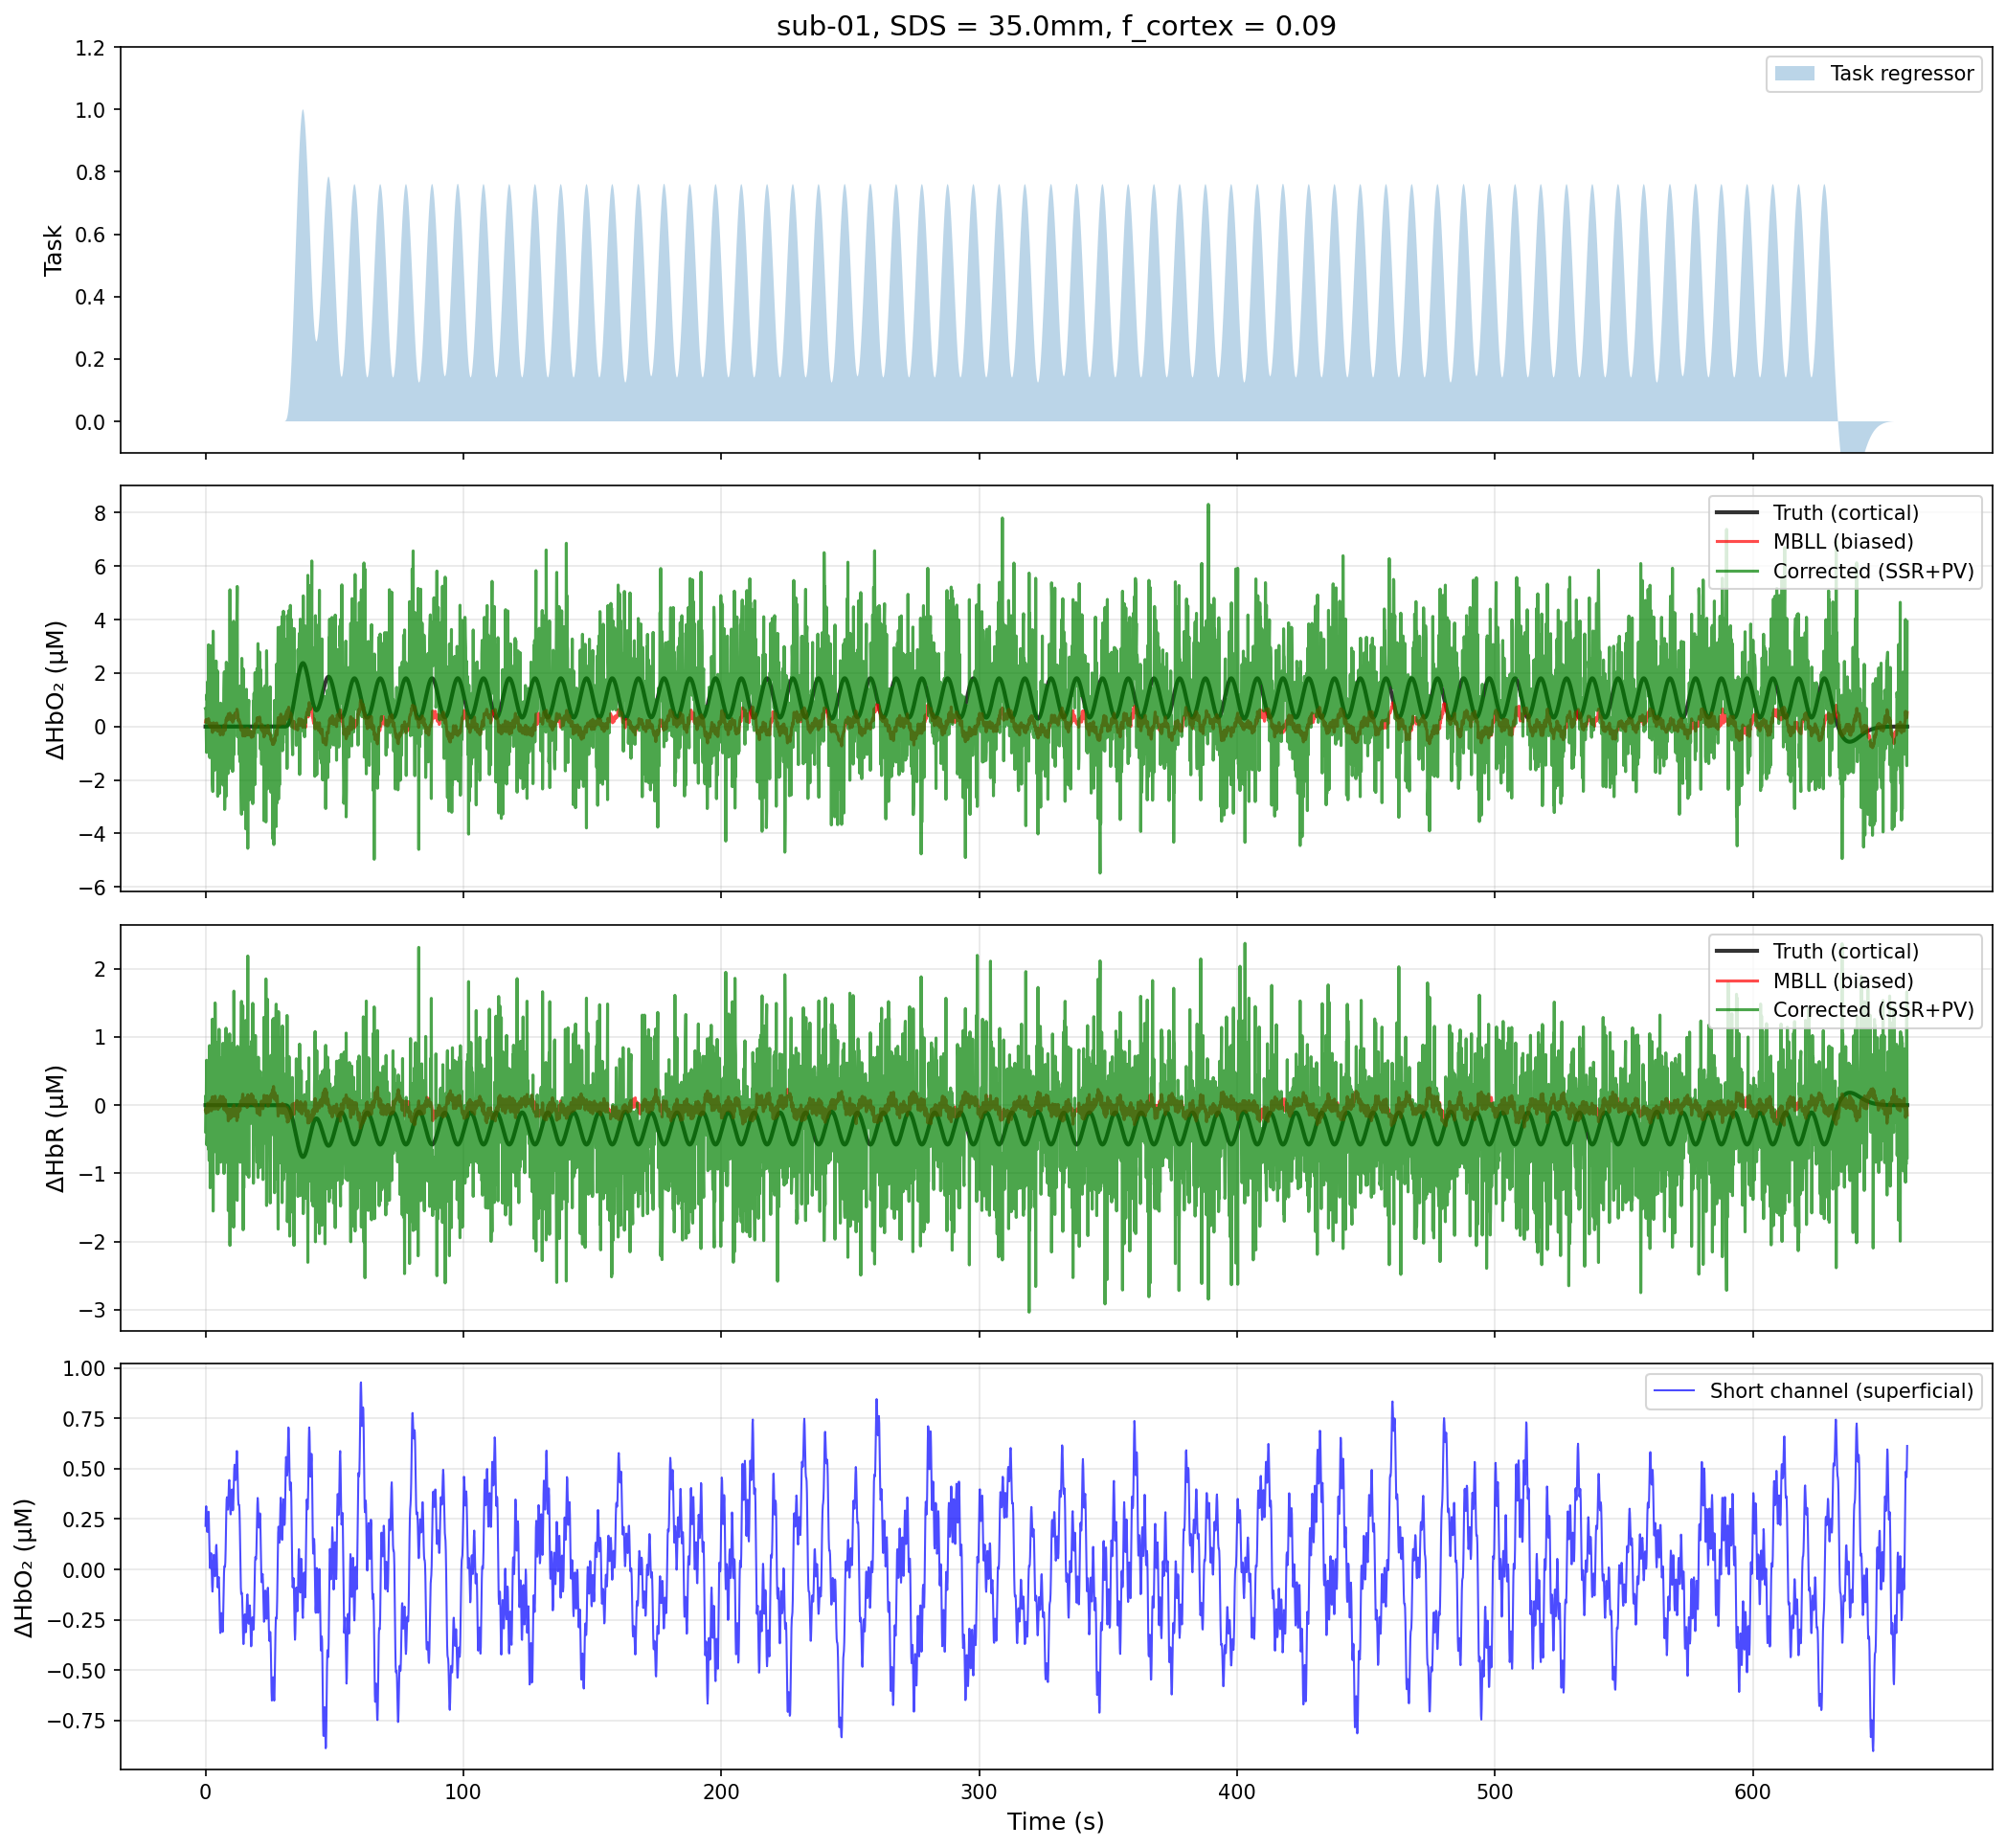
\includegraphics[width=\textwidth]{figures/figure1_timeseries.png}
\caption{Example synthetic fNIRS time series for a single subject at 35\,mm source-detector separation. From top: (1)~task regressor with shaded block periods; (2)~ground-truth cortical $\Delta[\mathrm{HbO}_2]$ (black), raw MBLL estimate (red) and the $\kappa$-corrected estimate (green); (3)~the same comparison for $\Delta[\mathrm{HbR}]$; (4)~short-separation channel representing superficial physiology. All comparison traces are full time series shown on equal footing: the corrected trace is the \emph{actual} SSR$+$partial-volume-corrected signal (not an amplitude$\times$design reconstruction), so the partial-volume factor $\kappa_{\mathrm{PV}}\!\approx\!11$ at this separation amplifies both signal and measurement noise in $\Delta[\mathrm{HbO}_2]$ and $\Delta[\mathrm{HbR}]$ alike. The task-locked amplitude (the GLM $\beta$ used in the error metrics, recovered by block averaging) moves toward the truth even though the single-trial trace is noisy; this noise amplification at shorter SDS is why the framework is scoped to long separations (Section~\ref{sec:scope}) and relies on block/trial averaging.}
\label{fig:timeseries}
\end{figure}

\subsection{Cortical sensitivity analysis}

The converged (Monte-Carlo) cortical sensitivity fractions $f_{\mathrm{cortex}}$ increased monotonically with SDS (table~\ref{tab:results}), consistent with deeper photon penetration at larger separations\cite{r10,r12}. At 25\,mm, only 4.3\% of the channel sensitivity originated from the cortex; this rose to 11.0\% at 40\,mm. These small fractions (an order of magnitude below what an under-converged analytical kernel returns (Section~\ref{sec:hankel_instab})) imply large partial-volume factors ($\kappa_{\mathrm{PV}} \approx 9$--$23$) and are central to the results that follow.

\subsection{Quantitative results: HbO$_2$}

Table~\ref{tab:results} presents the correction factors and error metrics for each SDS. The partial volume correction $\kappa_{\mathrm{PV}} = 1/f_{\mathrm{cortex}}$ ranged from 9.1 (40\,mm) to 23.4 (25\,mm), confirming that partial volume dilution is by far the dominant source of MBLL bias. The SSR diagnostic is strongly wavelength-dependent: $\kappa_{\mathrm{SSR}}(760\,\mathrm{nm}) \approx 1.2$ while $\kappa_{\mathrm{SSR}}(850\,\mathrm{nm}) \approx 9.8$--$10.6$ across separations, so a single cross-wavelength value is not meaningful. This factor is reported only as a diagnostic of residual systemic contamination: in the synthetic pipeline the simulated short channel is purely superficial, so SSR removes no cortical signal and only $\kappa_{\mathrm{PV}}$ is applied to the data (Section~\ref{sec:kappa_ssr_diag}). The error metrics reveal a strong separation dependence that is the central finding of this validation: the correction is beneficial at long SDS but harmful at the shortest, as detailed below.

\begin{table}[ht]
\centering
\caption{Correction factors and HbO$_2$ error metrics by source-detector separation. The corrected pipeline applies OD-level SSR followed by partial-volume scaling and MBLL inversion. In this synthetic validation only $\kappa_{\mathrm{PV}}$ is applied to the data; $\kappa_{\mathrm{SSR}}$ is reported as a diagnostic, because the simulated short channel is purely superficial and SSR therefore removes no cortical signal requiring restoration (see text). The $f_{\mathrm{cortex}}$ column is the wavelength-averaged fraction (mean of the 760 and 850\,nm values); the single-wavelength 760\,nm values used elsewhere (e.g.\ Supplementary Table~\ref{tab:snr}) are marginally smaller (0.041 at 25\,mm).}
\label{tab:results}
\begin{tabular}{@{}ccccccc@{}}
\toprule
\textbf{SDS} & $f_{\mathrm{cortex}}$ & $\kappa_{\mathrm{PV}}$ & $\kappa_{\mathrm{SSR}}$(760) & $\kappa_{\mathrm{SSR}}$(850) & \textbf{RMSE}$_{\mathrm{MBLL}}$ & \textbf{RMSE}$_{\mathrm{corr}}$ \\
\textbf{(mm)} & & & & & ($\mu$M) & ($\mu$M) \\
\midrule
25 & 0.043 & 23.42 & 1.17 & 9.82 & 2.105 & 3.270 \\
30 & 0.064 & 15.54 & 1.19 & 10.15 & 2.059 & 2.002 \\
35 & 0.091 & 11.02 & 1.22 & 10.52 & 1.992 & 1.228 \\
38 & 0.102 & 9.76 & 1.22 & 10.64 & 1.977 & 1.102 \\
40 & 0.110 & 9.12 & 1.21 & 10.52 & 1.966 & 1.087 \\
\midrule
\textbf{Overall} & & \textbf{13.77} & \textbf{1.20} & \textbf{10.33} & \textbf{2.020} & \textbf{1.929} \\
\bottomrule
\end{tabular}
\end{table}

\subsubsection{Operating regime: the correction is reliable only at long separations.}
\label{sec:scope}
In the self-consistent scenario (data and correction sharing the same Monte-Carlo $f_{\mathrm{cortex}}$), the HbO$_2$ RMSE improvement depends strongly on separation:
\begin{equation}
\mathrm{Improvement}_{\mathrm{HbO_2}}(\mathrm{SDS}) = -55\%,\; +3\%,\; +38\%,\; +44\%,\; +45\%\;\text{ at } 25, 30, 35, 38, 40\,\text{mm.}
\label{eq:improvement_hbo2}
\end{equation}
The pooled RMSE improvements above are computed over all five subjects; the benefit is consistent in sign across subjects, though variable in magnitude. Expressed as the per-subject improvement (mean\,$\pm$\,SD of $1-|\hat{\beta}-\beta|_{\mathrm{corr}}/|\hat{\beta}-\beta|_{\mathrm{MBLL}}$ across the five subjects), it is $41\pm19\%$ (HbO$_2$) and $89\pm5\%$ (HbR) at 38\,mm, and $41\pm20\%$ (HbO$_2$) and $82\pm6\%$ (HbR) at 40\,mm; every subject improves at long SDS. At long separations ($\geq$\,38\,mm) the correction reduces HbO$_2$ RMSE by 44--45\% (1.98 to 1.10\,$\mu$M at 38\,mm). At the shortest separation it is actively harmful: the corrected RMSE (3.27\,$\mu$M) \emph{exceeds} the uncorrected MBLL error (2.11\,$\mu$M). The cause is fundamental rather than a tuning artifact. With the converged $f_{\mathrm{cortex}}$, the cortical HbO$_2$ contribution to the measured optical density at 25\,mm is $\Delta\mathrm{OD}_{\mathrm{cortex}} \approx 9.6\times10^{-4}$, at or below the shot-noise floor ($\sigma_{\mathrm{OD}} = 1\times10^{-3}$, signal-to-noise ratio $\approx 0.96$); since $\kappa_{\mathrm{PV}} = 1/f_{\mathrm{cortex}}$ multiplies signal and noise equally, amplifying a near-noise-floor signal by $\approx$\,24 (the 760\,nm value; the wavelength-mean $\kappa_{\mathrm{PV}}$ in Table~\ref{tab:results} is 23.4) inflates the noise without recovering the signal (Supplementary Table~\ref{tab:snr}). The cortical SNR rises with separation (to $\approx$\,4 at 40\,mm, where $\kappa_{\mathrm{PV}} \approx 9$), which is why the correction becomes beneficial there. The pooled ``overall'' improvement (4.5\%) is therefore not a meaningful summary (it averages a harmful short-SDS regime with a beneficial long-SDS one) and we report the framework as a \emph{long-separation} method throughout. This threshold is \emph{noise-conditional}, not universal: the synthetic model assigns a fixed $\sigma_{\mathrm{OD}}=10^{-3}$ at every separation and channel, whereas real continuous-wave shot noise grows with source--detector separation as the detected intensity falls, so the exact crossover depends on the instrument. Under the simulated geometry and $\sigma_{\mathrm{OD}}=10^{-3}$, reliable improvement emerges at approximately 38--40\,mm; a lower-noise system would extend the usable range to shorter SDS and a noisier one would push it longer. The general statement of this result is therefore a two-dimensional SDS-versus-noise operating map rather than a single universal cutoff. The model-mismatch scenario at 38\,mm (Section~\ref{sec:mismatch}) achieved $+$70.3\% HbO$_2$ improvement when matched and $+$33.7\% when the CSF light-piping was ignored (table~\ref{tab:mismatch}), so geometry error roughly halves the long-SDS benefit but does not reverse it.



Supplementary Table~\ref{tab:kappa_stats} provides summary statistics for the correction factors across all subjects and channels.



\subsection{Quantitative results: HbR}

The correction framework was also evaluated for deoxygenated hemoglobin (HbR). Table~\ref{tab:hbr} presents the HbR-specific error metrics. The overall HbR RMSE improved from 0.653\,$\mu$M (MBLL) to 0.183\,$\mu$M (corrected), a 72.0\% improvement. Unlike HbO$_2$, the HbR correction is positive across the full separation range, including the short separations where HbO$_2$ correction fails (table~\ref{tab:hbr}): the improvement rises from 48.9\% at 25\,mm to a maximum of 89.8\% at 35\,mm and remains 82--89\% at 38--40\,mm. The apparent HbR advantage at short SDS is a secondary noise-propagation artifact of the $2\times2$ MBLL inverse and should not be read as a reason to use short separations: the extinction-coefficient matrix maps the two-wavelength optical-density noise onto the HbO$_2$ and HbR estimates with different gains, and for the coefficients used here the propagated noise happens to be smaller in the HbR estimate, so HbR is not limited by the noise floor that constrains HbO$_2$ at 25\,mm. Because the framework is scoped to long SDS by the HbO$_2$ limit (Section~\ref{sec:scope}), we report HbR improvement in the long-SDS regime (82--89\%), where both chromophores genuinely benefit, and do not otherwise rely on the short-SDS HbR behaviour.

\begin{table}[ht]
\centering
\caption{HbR error metrics by source-detector separation. The corrected pipeline applies OD-level SSR followed by partial-volume scaling and MBLL inversion; $\kappa$ factors quantify the net correction magnitude.}
\label{tab:hbr}
\begin{tabular}{@{}ccccc@{}}
\toprule
\textbf{SDS} & \textbf{RMSE}$_{\mathrm{MBLL}}$ & \textbf{RMSE}$_{\mathrm{corr}}$ & \textbf{Improvement} & \\
\textbf{(mm)} & ($\mu$M) & ($\mu$M) & (\%) & \\
\midrule
25 & 0.681 & 0.348 & 48.9 & \\
30 & 0.666 & 0.153 & 77.1 & \\
35 & 0.643 & 0.066 & 89.8 & \\
38 & 0.639 & 0.073 & 88.5 & \\
40 & 0.635 & 0.113 & 82.2 & \\
\midrule
\textbf{Overall} & \textbf{0.653} & \textbf{0.183} & \textbf{72.0} & \\
\bottomrule
\end{tabular}
\end{table}

\subsection{Inter-subject variability}

Supplementary Table~\ref{tab:subject_var} characterizes the variability in corrected HbO$_2$ amplitude estimates across the 5 simulated subjects.



The true peak cortical HbO$_2$ amplitude was $2.5$\,$\mu$M (with $\pm$20\% inter-subject variation). The mean $\beta$ values and their dispersion both shrink monotonically with separation, from $5.05 \pm 2.53$\,$\mu$M at 25\,mm to $3.34 \pm 1.02$\,$\mu$M at 40\,mm. At short separations the large partial-volume factor ($\kappa_{\mathrm{PV}} \approx 16$--$23$) amplifies measurement noise, inflating both the mean estimate and its inter-subject variance well above the truth; at long separations the estimate settles toward the true amplitude (a residual $\sim$30\% positive bias remains, reflecting imperfect cortical/systemic separation in the 5\,s block design). The error range narrows almost three-fold from 25 to 40\,mm (5.51 to 1.98\,$\mu$M), directly reinforcing the recommendation to restrict the correction to long separations.

\subsection{Visual summary}

Figure~\ref{fig:summary} presents a six-panel overview of the framework performance. Panel~(A) shows the monotonic increase of $f_{\mathrm{cortex}}$ with SDS (Monte-Carlo values). Panel~(B) shows the corresponding decrease of $\kappa_{\mathrm{PV}}$ from $\approx$\,23 to $\approx$\,9. Panel~(C) compares estimation errors before and after correction as a function of SDS, showing the crossover from harmful (25\,mm) to beneficial ($\geq$\,35\,mm). Panel~(D) plots estimated versus true cortical $\Delta[\mathrm{HbO}_2]$ amplitudes at long SDS, showing that MBLL estimates (red) fall well below the identity line while corrected estimates (green) are closer to it. Panel~(E) shows the applied $\kappa_{\mathrm{PV}}$ and the $\kappa_{\mathrm{SSR}}$ diagnostic at each SDS. Panel~(F) summarizes the separation-dependent HbO$_2$ RMSE reduction ($+$44--45\% at 38--40\,mm; $-$55\% at 25\,mm).

\begin{figure}[ht]
\centering
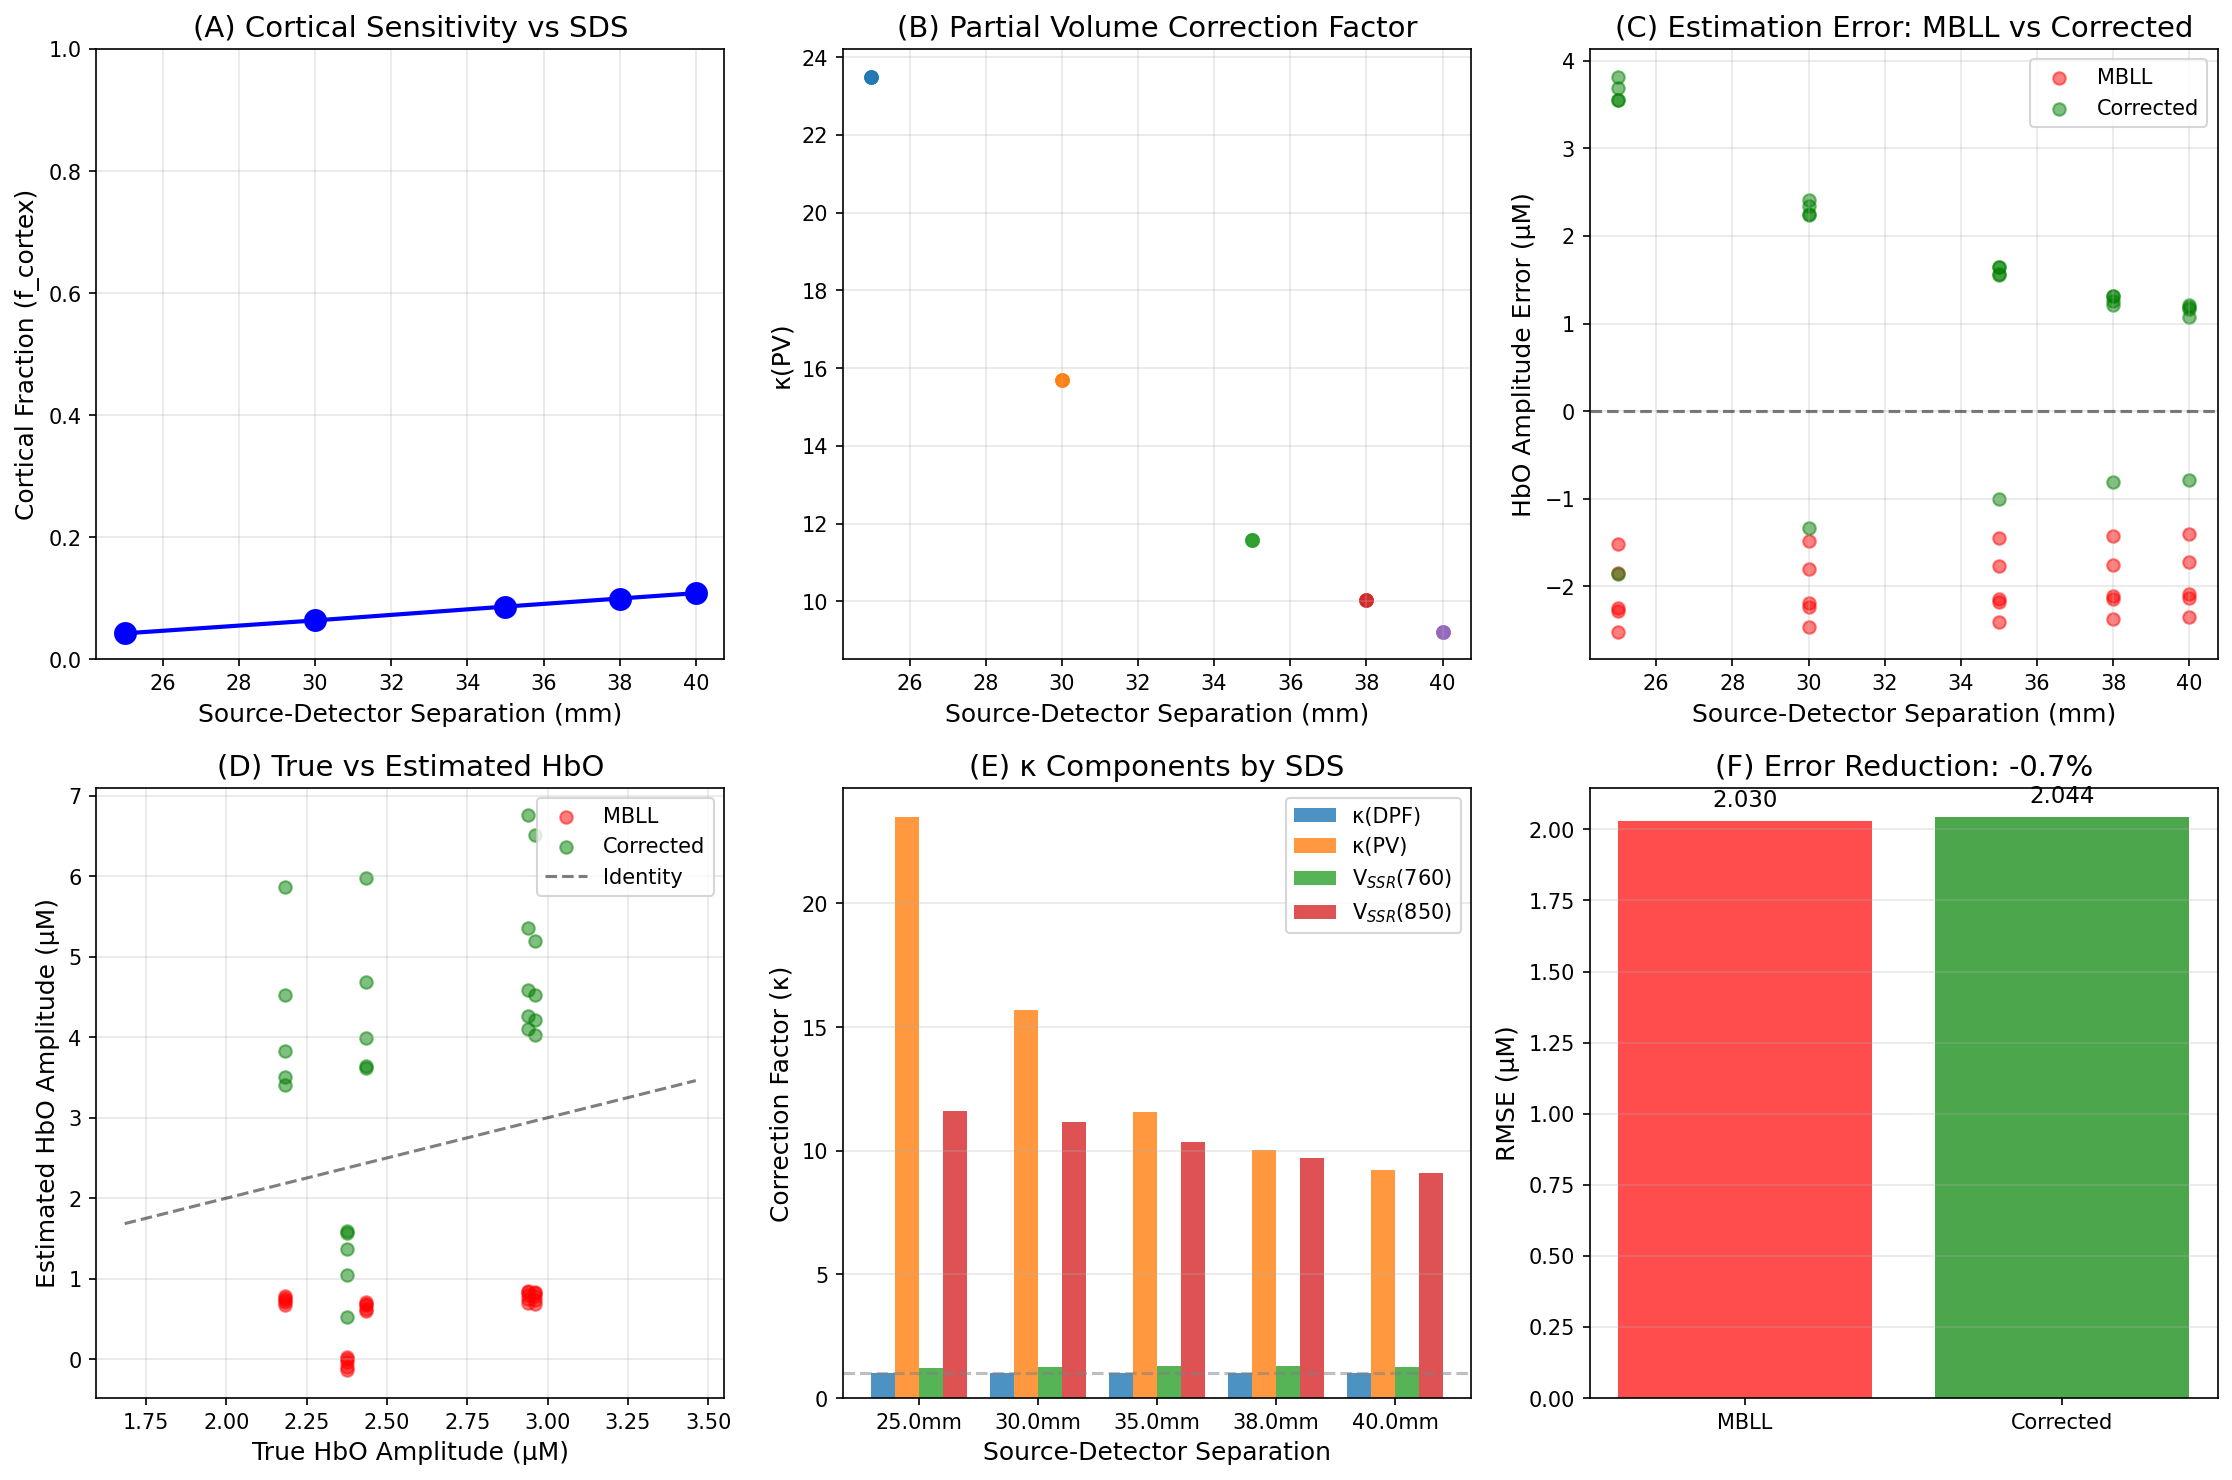
\includegraphics[width=\textwidth]{figures/figure2_summary.png}
\caption{Summary of $\kappa$ correction framework results (converged Monte-Carlo $f_{\mathrm{cortex}}$). (A)~Cortical sensitivity fraction versus SDS. (B)~Partial volume correction factor versus SDS. (C)~Estimation error (MBLL versus corrected) as a function of SDS, showing the harmful-to-beneficial crossover. (D)~True versus estimated cortical $\Delta[\mathrm{HbO}_2]$ amplitudes at long SDS. (E)~Applied $\kappa_{\mathrm{PV}}$ and $\kappa_{\mathrm{SSR}}$ diagnostic by SDS. (F)~Separation-dependent HbO$_2$ RMSE reduction (beneficial only at long SDS).}
\label{fig:summary}
\end{figure}

\subsection{Sensitivity to model assumptions}

\subsubsection{Superficial layer thickness.}
Figure~\ref{fig:robustness}(A, B) shows the dependence of $f_{\mathrm{cortex}}$ and $\kappa_{\mathrm{PV}}$ on assumed superficial layer thickness at SDS~$=$~30\,mm, computed with the converged Monte Carlo. As the superficial layer thickness increased from 8 to 14\,mm, $f_{\mathrm{cortex}}$ decreased from 0.239 to 0.030 while $\kappa_{\mathrm{PV}}$ increased from 4.2 to 33. A 2\,mm error in the assumed thickness (12$\rightarrow$14\,mm) more than halved $f_{\mathrm{cortex}}$ (0.063 to 0.030, a 52\% change) and doubled $\kappa_{\mathrm{PV}}$ (15.5 to 33, $+$114\%). This very strong sensitivity (steeper than the analytical kernel had suggested) underscores that accurate superficial-layer thickness (ideally a subject-specific estimate from the structural scan or an aged-matched template) is the single most important input to the correction, particularly for populations with atypical scalp-skull anatomy (neonates, elderly individuals, or patients with cranial abnormalities).

\subsubsection{Optical properties.}
Figure~\ref{fig:robustness}(C, D) illustrates the sensitivity of $f_{\mathrm{cortex}}$ and $\kappa_{\mathrm{PV}}$ to variations in cortical optical properties, computed with the converged two-layer Monte Carlo (\texttt{mc\_2layer.py}) at 30\,mm (the $\mu_a$ curve uses correlated reweighting of a single photon ensemble, so it is low-variance). A $\pm$30\% variation in cortical $\mu_a$ produced $\kappa_{\mathrm{PV}}$ changes of $-$32\% to $+$39\%; a $\pm$30\% variation in $\mu_s'$ produced $\kappa_{\mathrm{PV}}$ changes of $-$12\% to $+$20\%. Absorption is the dominant optical input, consistent with $\kappa_{\mathrm{PV}} = 1/f_{\mathrm{cortex}}$ tracking the survival-weighted cortical pathlength; both responses are monotonic and nearly symmetric. These optical-property sensitivities are larger than a naively evaluated analytical kernel suggests, but they remain smaller than the geometric sensitivity: a $\pm$2\,mm error in superficial-layer thickness changes $\kappa_{\mathrm{PV}}$ by more than 100\% (Figure~\ref{fig:robustness}A, B), so superficial-layer thickness remains the dominant input to $f_{\mathrm{cortex}}$, with cortical $\mu_a$ a clear second. For continuous-wave systems relying on literature optical properties rather than \textit{in vivo} estimates, this argues for reporting $\kappa_{\mathrm{PV}}$ with an explicit optical-property uncertainty band.

\begin{figure}[ht]
\centering
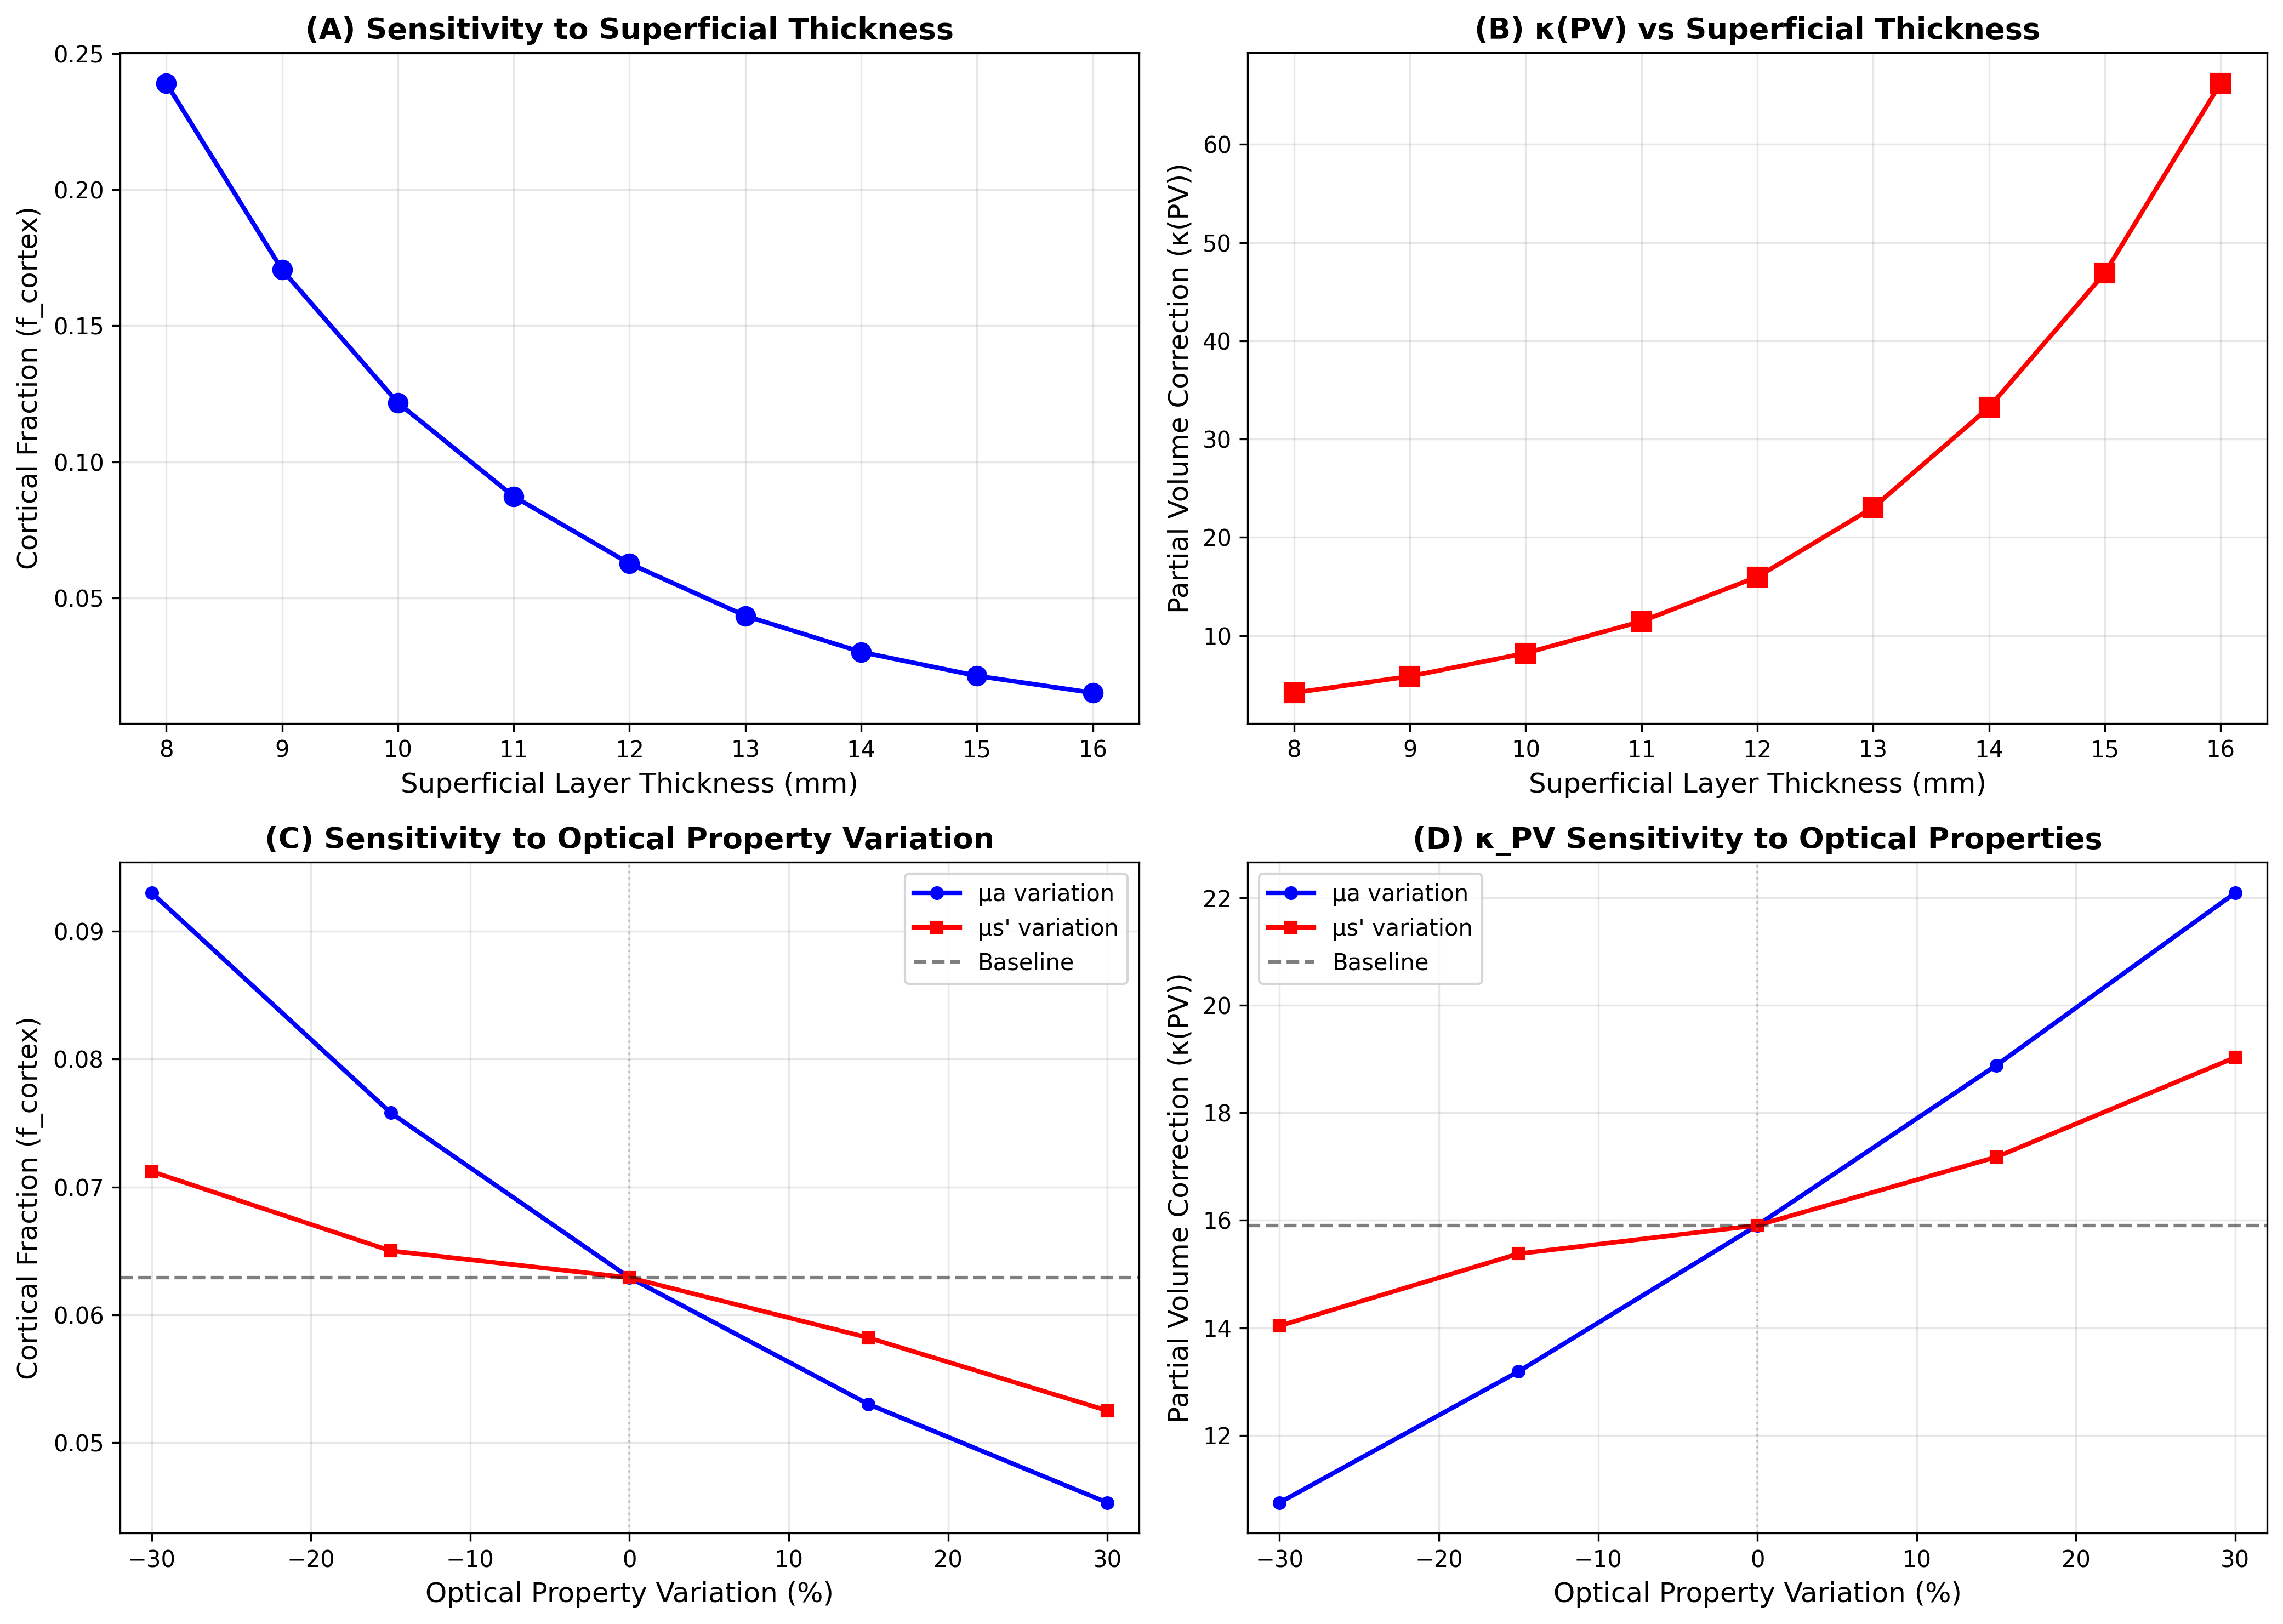
\includegraphics[width=\textwidth]{figures/figure3_robustness.png}
\caption{Sensitivity analysis of the correction framework. (A)~$f_{\mathrm{cortex}}$ versus assumed superficial layer thickness. (B)~$\kappa_{\mathrm{PV}}$ versus superficial layer thickness. (C)~$f_{\mathrm{cortex}}$ as a function of cortical optical property perturbation, sweeping $\mu_a$ and $\mu_s'$ independently from $-$30\% to $+$30\% of their nominal values. (D)~$\kappa_{\mathrm{PV}}$ versus the same optical property perturbation. Panels (C, D) are from the converged two-layer Monte Carlo (\texttt{mc\_2layer.py}); the $\mu_a$ sweep uses correlated reweighting of a single photon ensemble. Dashed lines indicate baseline values. All analyses at SDS\,$=$\,30\,mm, $\lambda = 760$\,nm.}
\label{fig:robustness}
\end{figure}

\subsubsection{Grid convergence and the dominant quadrature error.}
\label{sec:convergence_results}
The spatial grid convergence study varied $\Delta x$ (lateral, along S-D axis) and $\Delta z$ (depth) on a $4 \times 4$ grid while keeping $\Delta y = 2.0$\,mm and $y_{\max} = 50$\,mm fixed. With respect to the \emph{spatial} grid the integral is well-converged: at the standard resolution ($\Delta x = 1.0$\,mm, $\Delta z = 0.5$\,mm) the value deviates by $<$0.02\% from the finest-grid reference ($\Delta x = 0.25$\,mm, $\Delta z = 0.10$\,mm), and coarser grids ($\Delta x = 2.0$\,mm) introduce only $\sim$0.1--0.2\% bias. Critically, however, this study held the \emph{Hankel} quadrature ($n_s$, $s_{\max}$) fixed, and it is that quadrature (not the spatial grid) that controls the dominant error in $f_{\mathrm{cortex}}$ (Section~\ref{sec:hankel_instab}): the apparently ``converged'' spatial value sits on a Hankel-quadrature plateau that is itself far from the converged answer. This is why we calibrate $f_{\mathrm{cortex}}$ against Monte Carlo rather than rely on the analytical kernel's spatial-grid convergence. The lesson is general: spatial-grid convergence of a Jacobian integral does not certify convergence of the underlying spectral transform.

\subsubsection{Computational efficiency.}
A single 3D sensitivity computation (Hankel transform plus full Jacobian volume integration) required $3.12 \pm 0.01$\,s (mean $\pm$ std over 3 trials) per channel at the standard grid resolution ($\Delta x = 1.0$\,mm, $\Delta z = 0.5$\,mm, $\Delta y = 2.0$\,mm). Extrapolating to a full fNIRS session with 40 channels and 2 wavelengths yields an estimated total processing time of approximately 250\,s, which is practical for offline applications. This computational efficiency is orders of magnitude faster than Monte Carlo methods, which typically require minutes to hours for comparable sensitivity calculations\cite{r20}, while maintaining the full physical accuracy of the two-layer diffusion solution.

\subsection{Independent validation of the Kienle solution}
\label{sec:validation_results}

\subsubsection{Homogeneous-limit validation.}
When both layers were assigned identical optical properties, the Kienle two-layer solution computed via adaptive quadrature agreed with the closed-form semi-infinite fluence (equation~\ref{eq:fluence}) to within 0.01\% for lateral distances $\rho \leq 30$\,mm. This confirms that the Hankel-domain spectral function and numerical inversion are correctly implemented and that the two-layer solution reduces exactly to the known analytical limit. We note that the fixed-point trapezoid rule used in the main simulation pipeline (500 quadrature points, $s_{\max} = 30$\,mm$^{-1}$) showed larger deviations at $\rho > 20$\,mm due to under-resolved Bessel function oscillations; however, this does not affect the self-consistency of the main simulation, which uses the same Hankel implementation for both forward model and correction factor computation.

\subsubsection{Finite-difference cross-validation.}
Supplementary Table~\ref{tab:fd_validation} compares the cortical sensitivity fractions computed independently by the Kienle analytical solution (with adaptive quadrature and 3D cylindrical integration) and the FD numerical solver. The two methods agreed to within 9-11\%, with the FD solver producing systematically higher $f_{\mathrm{cortex}}$ values. This level of agreement is consistent with the known limitations of each approach: the FD solver introduces discretization error from the finite grid, while the Kienle solution assumes idealized planar layer boundaries. The agreement confirms that both methods capture the same underlying physics and that the Kienle-derived $f_{\mathrm{cortex}}$ values are quantitatively reliable.



\subsection{Effect of CSF layer on cortical sensitivity}
\label{sec:csf_results}

A white Monte Carlo simulation of the three-layer geometry (the diffusion approximation is invalid in the near-transparent CSF layer) shows that the explicit CSF layer \textit{increases} the cortical sensitivity fraction relative to the two-layer model (table~\ref{tab:three_layer}), the well-known CSF light-piping effect. The amplification factor $\gamma = f_{\mathrm{cortex}}^{\mathrm{3L}}/f_{\mathrm{cortex}}^{\mathrm{2L}}$, computed with the \emph{same} anisotropic (Henyey--Greenstein, $g=0.9$) transport as the two-layer model and averaged over independent seeds (nominal 2\,mm CSF), is $1.85\pm0.09$ at 25\,mm, $1.75\pm0.05$ at 30\,mm, $1.71\pm0.23$ at 35\,mm and $1.48\pm0.16$ at 40\,mm---a 45--85\% increase that diminishes with separation as the two-layer cortical fraction itself grows. These anisotropic values agree with an earlier isotropic-equivalent estimate within Monte-Carlo uncertainty, confirming that the ratio is robust to the scattering-anisotropy assumption. The low scattering of CSF lets photons traverse the layer with little attenuation and reach cortex that would otherwise be absorbed in the superficial tissue. We apply the ratio $\gamma$ to the converged two-layer fractions of table~\ref{tab:results}: $f_{\mathrm{cortex}}^{\mathrm{3L}} = \gamma\,f_{\mathrm{cortex}}^{\mathrm{2L}} \approx 0.076$, $0.110$, $0.147$ and $0.163$ at 25, 30, 35 and 40\,mm. The ratio depends on assumed CSF thickness (a thinner 1\,mm layer gives a smaller $\gamma\approx1.3$--$1.45$; the CSF thickness sweep is emitted by \texttt{mc\_uncertainty.py}). Even with CSF light-piping the cortical fraction remains small ($\lesssim$\,0.17), so $\kappa_{\mathrm{PV}}$ stays large ($\gtrsim$\,6) and the partial-volume problem is not eliminated by including CSF; it is moderated by roughly the factor $\gamma$.

\begin{table}[ht]
\centering
\caption{Effect of an explicit CSF layer on cortical sensitivity, from white Monte Carlo using the same anisotropic (Henyey--Greenstein, $g=0.9$) transport as the two-layer model (\texttt{mc\_uncertainty.py}; nominal 2\,mm CSF; means over independent seeds, $\gamma$ SD shown). The low-scattering CSF layer \textit{increases} $f_{\mathrm{cortex}}$ (light-piping) by the ratio $\gamma = f_{\mathrm{cortex}}^{\mathrm{3L}}/f_{\mathrm{cortex}}^{\mathrm{2L}}$; $f_{\mathrm{cortex}}^{\mathrm{3L}} = \gamma\,f_{\mathrm{cortex}}^{\mathrm{2L}}$ is shown using the converged two-layer fractions (table~\ref{tab:results}) and remains small ($\lesssim$\,0.17). The ratio is consistent with an isotropic-equivalent estimate within uncertainty and depends on CSF thickness.}
\label{tab:three_layer}
\begin{tabular}{@{}ccccc@{}}
\toprule
\textbf{SDS (mm)} & $f_{\mathrm{cortex}}^{\mathrm{2L}}$ & $\gamma$ (MC) & $f_{\mathrm{cortex}}^{\mathrm{3L}}$ & \textbf{Change (\%)} \\
\midrule
25 & 0.041 & $1.85\pm0.09$ & 0.076 & $+$85 \\
30 & 0.063 & $1.75\pm0.05$ & 0.110 & $+$75 \\
35 & 0.086 & $1.71\pm0.23$ & 0.147 & $+$71 \\
40 & 0.110 & $1.48\pm0.16$ & 0.163 & $+$48 \\
\bottomrule
\end{tabular}
\end{table}

\subsection{Model mismatch: two-layer correction applied to three-layer anatomy}
\label{sec:mismatch_results}

Table~\ref{tab:mismatch} presents the RMSE results for the matched and mismatched correction scenarios, both at the representative long separation of 38\,mm (Section~\ref{sec:scope}). In the matched scenario (data and correction sharing the Monte-Carlo two-layer $f_{\mathrm{cortex}}$), the partial-volume correction reduced RMSE by 70.3\% for HbO$_2$ and 38.6\% for HbR, confirming the framework's effectiveness when the assumed model matches the true anatomy; the smaller HbR improvement reflects its lower signal-to-noise ratio. In the mismatched scenario (data generated with the CSF-augmented $f_{\mathrm{cortex}}^{\mathrm{3L}}$ but corrected with the two-layer value), the correction still improved both chromophores but by roughly half as much (HbO$_2$ $+$33.7\%, HbR $+$14.4\%). The degradation occurs because the CSF light-piping effect \textit{increases} the true cortical sensitivity (table~\ref{tab:three_layer}), so the two-layer model underestimates $f_{\mathrm{cortex}}$ and its $\kappa_{\mathrm{PV}} = 1/f_{\mathrm{cortex}}$ is too large, partially overshooting the true cortical amplitude, but at long SDS the residual benefit remains positive, indicating the framework degrades gracefully rather than catastrophically when CSF is omitted.

\begin{table}[ht]
\centering
\caption{Model mismatch analysis at SDS~$=$~38\,mm. Matched: data and correction share the Monte-Carlo two-layer $f_{\mathrm{cortex}}$. Mismatched: data generated with the CSF-augmented $f_{\mathrm{cortex}}^{\mathrm{3L}}=\gamma f_{\mathrm{cortex}}^{\mathrm{2L}}$ but corrected with the two-layer value. Both improve at long SDS; the mismatch roughly halves the benefit.}
\label{tab:mismatch}
\begin{tabular}{@{}lcccc@{}}
\toprule
& \multicolumn{2}{c}{\textbf{HbO$_2$ RMSE ($\mu$M)}} & \multicolumn{2}{c}{\textbf{HbR RMSE ($\mu$M)}} \\
\cmidrule(lr){2-3}\cmidrule(lr){4-5}
\textbf{Scenario} & MBLL & Corrected & MBLL & Corrected \\
\midrule
Matched (2L$\rightarrow$2L) & 2.246 & 0.667 & 0.713 & 0.438 \\
Mismatched (3L$\rightarrow$2L) & 2.121 & 1.406 & 0.676 & 0.578 \\
\bottomrule
\end{tabular}
\end{table}

This result highlights a critical practical consideration: the accuracy of the $\kappa$ correction depends not only on the quality of the forward model but also on the fidelity of the assumed tissue geometry. When the CSF layer is present but unmodeled, the two-layer correction partially overcorrects because the assumed $f_{\mathrm{cortex}}^{\mathrm{2L}}$ ($\approx$0.10 at 38\,mm) underestimates the true three-layer value ($\approx$0.15), yielding a $\kappa_{\mathrm{PV}}$ that is too large; at long SDS the net effect is a reduced but still positive improvement.

\subsection{Sensitivity to $f_{\mathrm{cortex}}$ error}
\label{sec:fcortex_sensitivity}

Supplementary Table~\ref{tab:fcortex_sens} shows how the correction performance varies as the assumed $f_{\mathrm{cortex}}$ deviates from its true value, at the representative long separation of 38\,mm. With the exact $f_{\mathrm{cortex}}$ ($\pm$0\% error), the matched correction achieves a 70.3\% HbO$_2$ (38.6\% HbR) RMSE reduction. The framework is robust to moderate errors: HbO$_2$ improvement remains above 64\% from $-$10\% to $+$20\% perturbation and above 50\% from $-$20\% to $+$30\%, falling to 35\% only at $-$30\%. Performance peaks near the correct value and degrades on either side; underestimating $f_{\mathrm{cortex}}$ (negative errors) inflates $\kappa_{\mathrm{PV}}$ and degrades the estimate faster than overestimating it, with HbR turning marginally negative ($-$3\%) only at the $-$30\% extreme. This tolerance is reassuring given the $\pm$2\,mm superficial-thickness uncertainty that dominates the $f_{\mathrm{cortex}}$ input.



Both chromophores are recovered best when the assumed $f_{\mathrm{cortex}}$ matches the truth, and performance degrades as the assumed value departs from it, falling off faster for underestimates, where the inflated $\kappa_{\mathrm{PV}}$ overcorrects and amplifies noise. HbR improvement is consistently smaller than HbO$_2$, reflecting the lower signal-to-noise ratio of the deoxy-hemoglobin channel, and remains positive except at the $-$30\% extreme. The broad plateau (HbO$_2$ $>$\,64\% across $-$10\% to $+$20\%) indicates the correction is forgiving of realistic $f_{\mathrm{cortex}}$ uncertainty once a converged forward model places it in the correct band.

\subsection{Pipeline demonstration: simulated finger-tapping paradigm}
\label{sec:pipeline_demo}

To visualise the complete pipeline operating end-to-end on a single channel, we simulated a finger-tapping paradigm using the idealized synthetic block configuration (60 blocks of 5\,s task / 5\,s rest, 7.8125\,Hz, 760/850\,nm, SDS~$=$~38\,mm; an idealization of the experiment, cf.\ Section~\ref{sec:realdata}) with a ground-truth cortical $\Delta[\mathrm{HbO}_2]$ of $+2.5\,\mu$M, physiological systemic oscillations, and shot noise; the cortical contribution to the long channel uses the converged $f_{\mathrm{cortex}}(760)=0.102$, $f_{\mathrm{cortex}}(850)=0.103$ ($\kappa_{\mathrm{PV}}=9.76$). The runnable script (NumPy/Matplotlib only) is provided as supplementary material.

This demonstration also makes the central limitation concrete. At the converged $f_{\mathrm{cortex}}\approx0.10$, the cortical signal is only $\sim$10\% of the long-channel sensitivity, so on a \emph{single} channel it sits close to the systemic and instrumental noise after dilution, exactly as the synthetic validation predicts at this separation (Section~\ref{sec:scope}). The partial-volume correction ($\kappa_{\mathrm{PV}}=9.76$) recovers the bulk of the diluted amplitude and reduces single-channel HbO$_2$ RMSE, but single-channel peak recovery is incomplete because short-separation regression also removes part of the small cortical signal. Robust quantitative recovery therefore relies on the channel- and trial-averaging used in the real-data analysis below (Section~\ref{sec:realdata}), where averaging over the contralateral long channels and the repeated tapping trials raises the effective SNR and the group-mean corrected amplitude reaches the physiological range. We thus treat this single-channel simulation as an illustrative walkthrough of the pipeline stages rather than as a quantitative performance claim; the quantitative claims rest on the multi-subject synthetic validation (Sections~\ref{sec:scope} and following) and the five-subject real data.

\subsection{Proof-of-concept demonstration on experimental human fNIRS data}
\label{sec:realdata}

To evaluate the $\kappa$-correction framework on real human measurements, we applied the complete pipeline to publicly available fNIRS data from the BIDS-NIRS-Tapping dataset\cite{r36}. Unlike the synthetic validation above, this analysis operates on genuine physiological signals with \emph{no ground truth}; it is therefore a proof-of-concept demonstration that tests whether the correction produces amplitudes consistent with known motor-cortex hemodynamics, not a measurement of its accuracy.

\subsubsection{Dataset and preprocessing.}

The BIDS-NIRS-Tapping dataset contains fNIRS recordings from five participants performing a finger-tapping task. The paradigm has \emph{three} conditions---left-hand tapping, right-hand tapping, and control---of 30 trials each (90 trials total), 5\,s per trial, with irregular inter-onset intervals of approximately 25--40\,s; data were acquired at 760 and 850\,nm. The probe covers both hemispheres and includes long-separation channels (median SDS $\approx$ 38\,mm) and short-separation channels (SDS $<$ 15\,mm), enabling per-wavelength SSR. Data were stored in SNIRF format following the BIDS-NIRS standard and loaded using MNE-Python and MNE-BIDS\cite{r37}.

We processed all five subjects (sub-01--sub-05) through an identical, upgraded pipeline (\texttt{fnirs\_kappa\_realdata\_v2.py}). The steps were: (1)~conversion from raw intensity to optical density; (2)~motion correction by temporal-derivative distribution repair (TDDR) and channel quality control by the scalp-coupling index (SCI), rejecting channels with SCI $<0.5$; (3)~bandpass filtering (0.01--0.1\,Hz, zero-phase); (4)~\emph{per-channel} short-separation regression at the OD level, using for each long channel the geometrically \emph{nearest} short channel (SDS $<15$\,mm) as the regressor, independently at 760 and 850\,nm, with the variance-removal diagnostic $\kappa_{\mathrm{SSR}}(\lambda) = 1/(1-R^2_{\mathrm{SS}}(\lambda))$ recorded but \emph{not} applied (Section~\ref{sec:kappa_ssr_diag}); (5)~\emph{per-channel} partial-volume correction, dividing each long channel's SSR-cleaned $\Delta\mathrm{OD}(\lambda)$ by its own $f_{\mathrm{cortex}}(\lambda,\mathrm{SDS})$ evaluated at that channel's actual separation (not a single median) from the CSF-augmented Monte-Carlo table ($f_{\mathrm{cortex}} = \gamma\,f_{\mathrm{cortex}}^{\mathrm{2L}}$, with the anisotropic CSF ratio $\gamma$ of Section~\ref{sec:csf_results}); (6)~per-channel MBLL inversion with wavelength-specific DPFs ($\mathrm{DPF}(760) = 6.15$, $\mathrm{DPF}(850) = 5.09$; Scholkmann and Wolf\cite{r14}) and the extinction coefficients of table~\ref{tab:extinction}, applied wavelength-by-wavelength as in equation~(\ref{eq:matrix_correction}). Because the paradigm has left- and right-hand conditions with contralateral spatial specificity, we block-averaged each condition separately (relative to a 5\,s pre-stimulus baseline) and analysed the \emph{contralateral} long channels (left-hand $\to$ right-hemisphere channels, $x>0$; right-hand $\to$ left-hemisphere, $x<0$; a convention confirmed by the observed lateralization, contralateral response $>$ ipsilateral for both hands). Response amplitudes were estimated as the \emph{mean} of the block-averaged response over a fixed, pre-registered window (HbO$_2$: 4--10\,s; HbR: 7--13\,s post-onset), which avoids the positive bias of a maximum after large amplification. The uncorrected pipeline omits steps (4)--(5). Per-subject results appear in table~\ref{tab:realdata_group}; figures~\ref{fig:realdata_timeseries}--\ref{fig:realdata_summary} illustrate Subject~01 and the amplification structure, and figure~\ref{fig:realdata_group} shows the group block average.

\subsubsection{Results.}

The upgraded per-channel, contralateral analysis for all five subjects is reported in table~\ref{tab:realdata_group}; figure~\ref{fig:realdata_summary} shows the group summary and figure~\ref{fig:realdata_timeseries} the per-subject amplification. All contralateral long channels lie at $\approx$38\,mm, within the reliable long-SDS regime (Section~\ref{sec:scope}); the per-channel CSF-augmented $f_{\mathrm{cortex}}\approx0.16$ gives a partial-volume factor $\kappa_{\mathrm{PV}}\approx6.3$, the dominant and only applied amplification. The nearest short channel provides SSR denoising and the per-wavelength $\kappa_{\mathrm{SSR}}$ variance diagnostic, which is not applied.

\begin{figure}[ht]
\centering
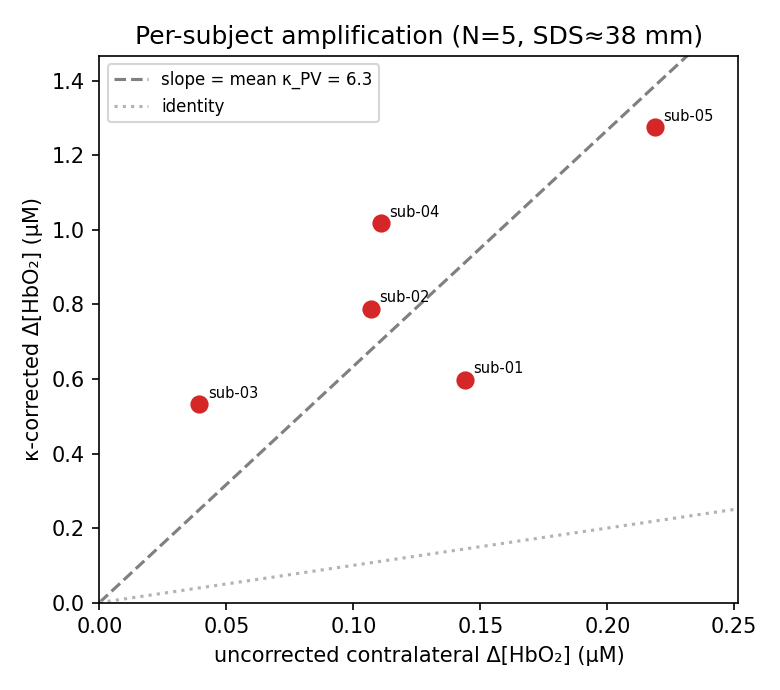
\includegraphics[width=0.6\textwidth]{figures/figure4_realdata_timeseries.png}
\caption{Per-subject amplification for the five BIDS-NIRS-Tapping subjects (contralateral long channels, SDS~$\approx$~38\,mm). Each point is one subject's uncorrected versus $\kappa$-corrected window-mean $\Delta[\mathrm{HbO}_2]$; the dashed line is the mean per-channel $\kappa_{\mathrm{PV}}\approx6.3$ (only applied amplification) and the dotted line is the identity. Per-subject net scaling varies (4--14$\times$) because the intervening SSR step removes a subject-specific fraction of the raw peak before $\kappa_{\mathrm{PV}}$ amplification.}
\label{fig:realdata_timeseries}
\end{figure}

For Subject~01 (table~\ref{tab:realdata}, figure~\ref{fig:realdata_hrf}) the contralateral block-averaged HbO$_2$ response rises during the task to an uncorrected window-mean of $+0.14\,\mu$M; after nearest-short SSR denoising and the applied per-channel partial-volume correction ($\kappa_{\mathrm{PV}}=6.28$) it reaches $+0.60\,\mu$M (a $4.2\times$ net amplification), while HbR deepens from $-0.030$ to $-0.167\,\mu$M. The corrected HbO$_2$ amplitude lies in the physiological range for motor-cortex finger tapping. Had the $\kappa_{\mathrm{SSR}}$ variance diagnostic (760: 1.97, 850: 2.78) been applied on top of $\kappa_{\mathrm{PV}}$, it would have inflated the estimate by roughly a further factor of two, above the physiological range---the concrete, checkable consequence of the statistical clarification in Section~\ref{sec:kappa_ssr_diag}.

\begin{figure}[ht]
\centering
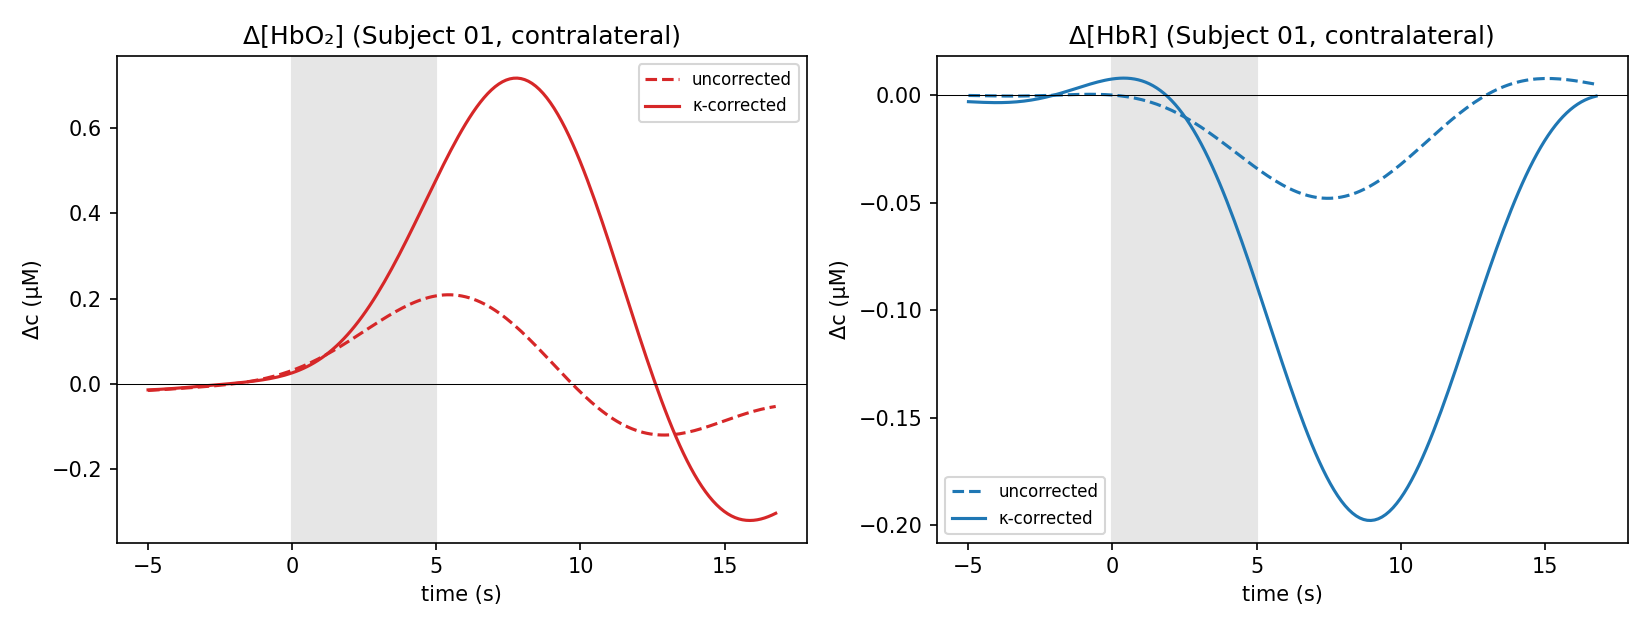
\includegraphics[width=\textwidth]{figures/figure5_realdata_hrf.png}
\caption{Contralateral block-averaged hemodynamic response (Subject~01, SDS~$\approx$~38\,mm), condition-resolved and averaged over the contralateral long channels. \textit{Left}: $\Delta[\mathrm{HbO}_2]$. \textit{Right}: $\Delta[\mathrm{HbR}]$. Uncorrected (dashed) versus $\kappa$-corrected (solid, per-channel $\kappa_{\mathrm{PV}}=6.28$ applied; $\kappa_{\mathrm{SSR}}$ diagnostic only). Grey shading indicates the 5\,s task period; amplitudes are estimated as the mean over a fixed response window.}
\label{fig:realdata_hrf}
\end{figure}

\begin{figure}[ht]
\centering
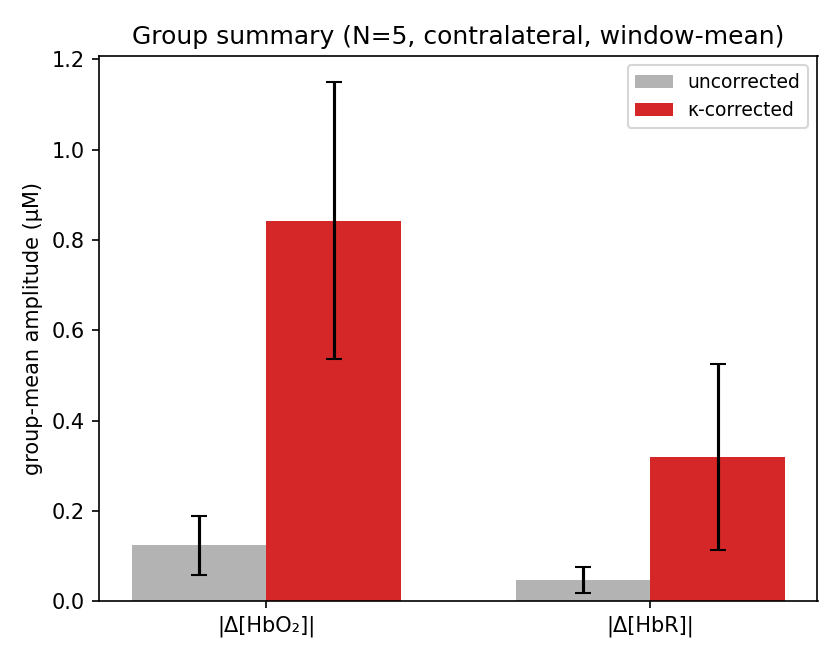
\includegraphics[width=0.62\textwidth]{figures/figure6_realdata_summary.png}
\caption{Group summary (N$=$5, contralateral, window-mean estimator). Group-mean $|\Delta[\mathrm{HbO}_2]|$ and $|\Delta[\mathrm{HbR}]|$ (error bars: SD across subjects), uncorrected versus $\kappa$-corrected; only $\kappa_{\mathrm{PV}}$ is applied.}
\label{fig:realdata_summary}
\end{figure}

\begin{table}[ht]
\centering
\caption{Upgraded in-vivo result for Subject~01 (BIDS-NIRS-Tapping): contralateral long channels ($n=20$ after SCI QC), condition-resolved, window-mean amplitudes at SDS~$\approx$~38\,mm. Only the per-channel $\kappa_{\mathrm{PV}}$ is applied; $\kappa_{\mathrm{SSR}}$ is a reported variance-removal diagnostic.}
\label{tab:realdata}
\begin{tabular}{@{}lcc@{}}
\toprule
\textbf{Metric} & \textbf{HbO$_2$} & \textbf{HbR} \\
\midrule
Uncorrected window-mean ($\mu$M) & $+0.144$ & $-0.030$ \\
$\kappa$-corrected window-mean ($\mu$M) & $+0.598$ & $-0.167$ \\
Net scaling factor & 4.15$\times$ & 5.6$\times$ \\
\midrule
$\kappa_{\mathrm{PV}}$ (mean per-channel, applied) & \multicolumn{2}{c}{6.28} \\
$\kappa_{\mathrm{SSR}}(760\,\mathrm{nm})$ (diagnostic) & \multicolumn{2}{c}{1.97} \\
$\kappa_{\mathrm{SSR}}(850\,\mathrm{nm})$ (diagnostic) & \multicolumn{2}{c}{2.78} \\
Contralateral channels ($n$) & \multicolumn{2}{c}{20} \\
Wavelengths & \multicolumn{2}{c}{760, 850\,nm} \\
Median SDS & \multicolumn{2}{c}{38.2\,mm} \\
\bottomrule
\end{tabular}
\end{table}

\subsubsection{Group-level results across all five subjects.}
\label{sec:realdata_group}

The same upgraded pipeline was applied to every participant (sub-01--sub-05). Per-subject metrics are in table~\ref{tab:realdata_group} and figure~\ref{fig:realdata_group} overlays the contralateral group block average. Because the applied $\kappa_{\mathrm{PV}} = 1/f_{\mathrm{cortex}}(\mathrm{SDS})$ depends only on each channel's separation and all contralateral long channels sit near 38\,mm, the per-channel mean $\kappa_{\mathrm{PV}}$ is nearly identical across subjects ($6.34\pm0.06$). The $\kappa_{\mathrm{SSR}}$ variance diagnostic, by contrast, is data-driven and wavelength-dependent, varying between subjects ($\kappa_{\mathrm{SSR}}(760\,\mathrm{nm}) = 1.78 \pm 0.15$, $\kappa_{\mathrm{SSR}}(850\,\mathrm{nm}) = 2.34 \pm 0.39$), reflecting how much long-channel variance the nearest short channel removed. Because the two wavelengths differ, $\kappa_{\mathrm{SSR}}$ is reported per wavelength rather than as a cross-wavelength mean.

\begin{table}[ht]
\centering
\caption{Per-subject and group-level results for the upgraded in-vivo analysis (N$=$5; contralateral long channels; condition-resolved; window-mean amplitudes; SDS $\approx$ 38\,mm). $\kappa_{\mathrm{PV}}$ is the mean per-channel applied factor; $\kappa_{\mathrm{SSR}}$ is a reported per-wavelength variance-removal diagnostic (not applied). $|\Delta[\mathrm{HbO}_2]|$ and $|\Delta[\mathrm{HbR}]|$ are group-referenced window-mean magnitudes; ``Mean scale'' is the average of the HbO$_2$ and HbR net scaling factors. Subject~01 is the case detailed in table~\ref{tab:realdata}.}
\label{tab:realdata_group}
\small
\begin{tabular}{@{}lcccccccc@{}}
\toprule
\textbf{Subject} & $\kappa_{\mathrm{PV}}$ & $\kappa_{\mathrm{SSR}}$(760) & $\kappa_{\mathrm{SSR}}$(850) &
\multicolumn{2}{c}{$|\Delta[\mathrm{HbO}_2]|$ ($\mu$M)} &
\multicolumn{2}{c}{$|\Delta[\mathrm{HbR}]|$ ($\mu$M)} & Mean \\
\cmidrule(lr){5-6}\cmidrule(lr){7-8}
 & & & & uncorr. & corr. & uncorr. & corr. & scale \\
\midrule
sub-01 & 6.28 & 1.97 & 2.78 & 0.144 & 0.598 & 0.030 & 0.167 & 4.9$\times$ \\
sub-02 & 6.36 & 1.83 & 2.10 & 0.107 & 0.789 & 0.023 & 0.158 & 7.1$\times$ \\
sub-03 & 6.37 & 1.64 & 2.36 & 0.039 & 0.533 & 0.023 & 0.186 & 10.9$\times$ \\
sub-04 & 6.28 & 1.86 & 2.62 & 0.111 & 1.019 & 0.080 & 0.583 & 8.2$\times$ \\
sub-05 & 6.41 & 1.61 & 1.82 & 0.219 & 1.275 & 0.076 & 0.501 & 6.2$\times$ \\
\midrule
Mean & 6.34 & 1.78 & 2.34 & 0.124 & 0.843 & 0.047 & 0.319 & 7.5$\times$ \\
SD & 0.06 & 0.15 & 0.39 & 0.065 & 0.307 & 0.029 & 0.206 & 2.2$\times$ \\
\bottomrule
\end{tabular}
\end{table}

\begin{figure}[ht]
\centering
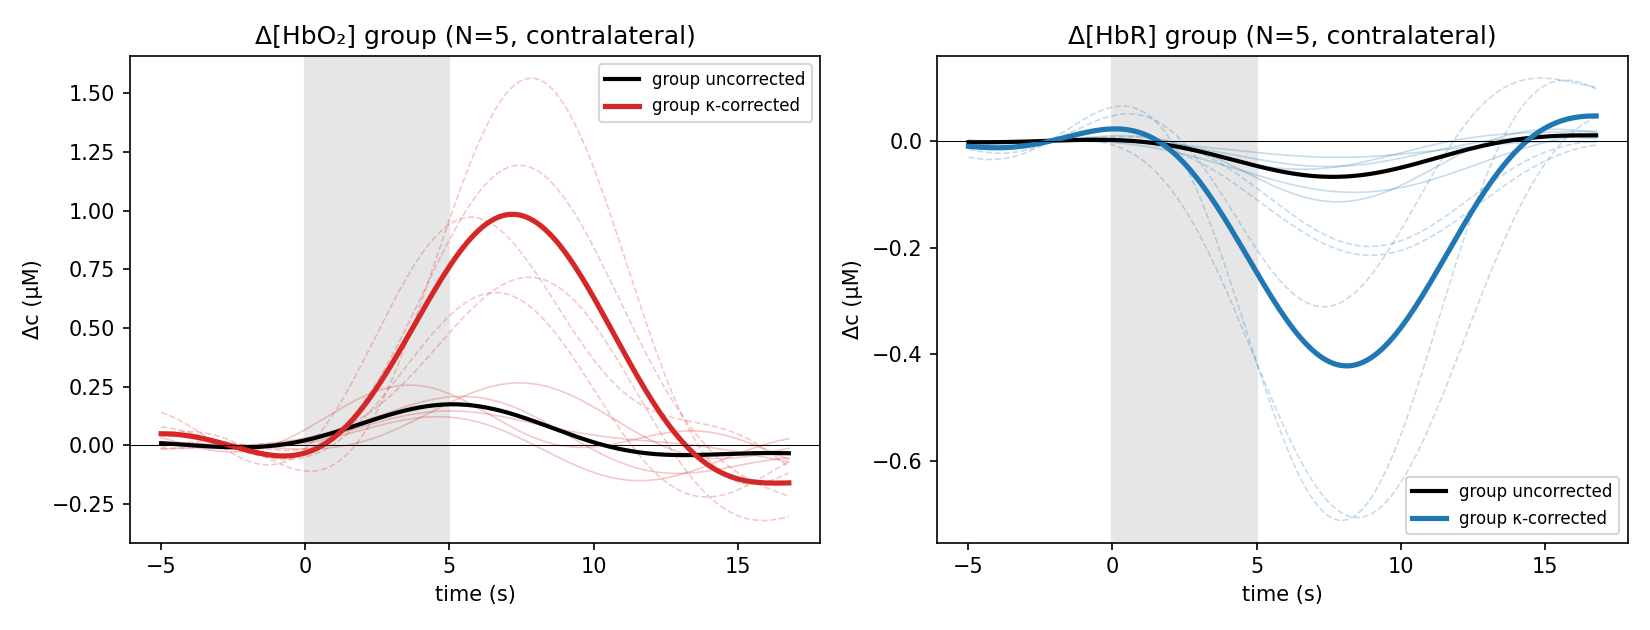
\includegraphics[width=\textwidth]{figures/figure7_group_block_average.png}
\caption{Group-level contralateral block-averaged hemodynamic response across all five BIDS-NIRS-Tapping subjects. Thin lines show per-subject contralateral means (solid = uncorrected, dashed = $\kappa$-corrected); bold lines show the group mean. No formal standard-error envelope is drawn---the spread of the thin per-subject lines conveys inter-subject variability. The applied per-channel partial-volume correction ($\kappa_{\mathrm{PV}}\approx6.3$) amplifies both HbO$_2$ and HbR in every subject; the group-mean corrected HbO$_2$ window-mean is $0.84\pm0.31\,\mu$M ($\sim$7$\times$ the uncorrected estimate), within the physiological range. $\kappa_{\mathrm{PV}}$ is nearly identical across subjects because they share the probe geometry; the net scaling varies with the per-subject SSR denoising (the $\kappa_{\mathrm{SSR}}$ diagnostic).}
\label{fig:realdata_group}
\end{figure}

The group-mean uncorrected contralateral HbO$_2$ ($0.124\pm0.065\,\mu$M) rises to $0.843\pm0.307\,\mu$M after correction (a $\sim$7$\times$ group amplification), and HbR from $-0.047$ to $-0.319\pm0.206\,\mu$M. All five corrected HbO$_2$ amplitudes (0.60, 0.79, 0.53, 1.02, 1.28\,$\mu$M) fall within the physiological range for motor-cortex finger tapping. With only five subjects and no concurrent ground truth, these are descriptive summaries (mean$\pm$SD across subjects); we make no inferential (hypothesis-testing) claim. Landing in the physiological range is a weak test on its own---many scaling factors would produce plausible amplitudes---so the load-bearing real-data result is the \emph{checkable, methodological} contrast: the same pipeline yields $\sim$0.8\,$\mu$M when $\kappa_{\mathrm{SSR}}$ is treated as a variance diagnostic and roughly twice that (above the physiological range) if $\kappa_{\mathrm{SSR}}$ is applied on top of $\kappa_{\mathrm{PV}}$, a direct and reproducible consequence of the statistical clarification in Section~\ref{sec:kappa_ssr_diag}. The per-subject net scaling varies (4--14$\times$) with how much of the raw peak the nearest-short SSR removed before amplification; subject~03, with the smallest uncorrected amplitude and the largest net scaling, warrants the most caution.

Importantly, these results illustrate the SDS-dependent operating regime of the correction framework, which the converged $f_{\mathrm{cortex}}$ inverts relative to a naive reading. Partial-volume dilution is severe at \emph{all} separations ($f_{\mathrm{cortex}} = 0.04$ to $0.11$, $\kappa_{\mathrm{PV}} = 9$ to $23$); $\kappa_{\mathrm{PV}}$ is the dominant correction throughout. What changes with separation is not the size of the dilution but whether the cortical signal is recoverable: at short SDS ($\leq$30\,mm) the diluted cortical optical density sits at or below the measurement-noise floor (Section~\ref{sec:scope}), so the large $\kappa_{\mathrm{PV}}$ amplifies noise and the correction is unreliable; at long SDS ($\geq$38\,mm) the cortical SNR is adequate and $\kappa_{\mathrm{PV}}$ recovers physiological amplitudes, as observed here. The real data sit at 38.3\,mm, in the reliable regime. $\kappa_{\mathrm{SSR}}(\lambda)$ is a variance-removal diagnostic and is not applied; $\kappa_{\mathrm{PV}}$ corrects the optical dilution of the cortical component that \emph{survives} SSR and does not attempt to reconstruct any cortical signal that SSR removed (Section~\ref{sec:kappa_ssr_diag}).

The uncorrected contralateral HbO$_2$ amplitude of ${\sim}0.12$\,$\mu$M lies in the sub-$\mu$M range typical of MBLL-derived motor-cortex finger-tapping responses reported by adult fNIRS studies\cite{r33,r34,r35}, reflecting the same partial-volume dilution that motivates this work. After nearest-short SSR denoising and the applied per-channel partial-volume correction, the group-mean corrected value of ${\sim}0.8$\,$\mu$M is consistent with the magnitude of cortical hemoglobin changes recovered after partial-volume correction in simultaneous fMRI/NIRS calibration studies\cite{r31,r32}. This demonstrates that the framework recovers physiologically plausible cortical hemodynamic amplitudes from real fNIRS measurements at long separations, subject to the demonstration-not-validation caveats above. The correction uses the CSF-augmented (three-layer) $f_{\mathrm{cortex}}\approx0.16$ ($\kappa_{\mathrm{PV}}\approx6.3$; Table~\ref{tab:three_layer}), appropriate for the CSF layer of the real head; the two-layer value ($f_{\mathrm{cortex}}\approx0.10$, $\kappa_{\mathrm{PV}}\approx9.7$) would give a larger $\approx1.3\,\mu$M (an upper bound that ignores CSF light-piping), so the physiological estimate is bracketed as $\approx0.8$--$1.3\,\mu$M.

\section{Discussion}

\subsection{Summary of findings}

This study shows, through synthetic validation with known ground truth and a proof-of-concept application to experimental data \emph{without} ground truth, that the systematic bias in MBLL-derived fNIRS concentration estimates can be characterized and corrected with the proposed $\kappa$ correction combined with SSR and a Monte-Carlo--calibrated sensitivity model, \emph{at long source--detector separations}. The key finding is that MBLL underestimates cortical hemoglobin changes by roughly an order of magnitude, because only a small fraction of the channel sensitivity ($f_{\mathrm{cortex}}\approx0.04$--$0.11$) originates from the cortex while MBLL assumes a uniform medium. Equally important is a boundary on applicability: because the cortical contribution is so small, at short separations ($\leq$30\,mm) the diluted cortical signal falls at or below the measurement-noise floor, and the large partial-volume factor amplifies noise rather than recovering signal. The framework is therefore a long-separation method.

In the multi-subject synthetic validation, the partial-volume correction reduces HbO$_2$ RMSE by 44--45\% at 38--40\,mm (and HbR by 82--89\%), while at 25\,mm it is harmful ($-$55\% for HbO$_2$). A separate, and consequential, methodological point concerns the SSR term: $\kappa_{\mathrm{SSR}}=1/(1-R^2_{\mathrm{SS}})$ is an inverse residual-\emph{variance} ratio, not an amplitude-restoration factor, so we report it as a variance-removal diagnostic and apply only $\kappa_{\mathrm{PV}}$; this keeps the real-data corrected amplitude physiological ($\sim$0.8\,$\mu$M) instead of the roughly twofold larger value that applying $\kappa_{\mathrm{SSR}}$ on top of $\kappa_{\mathrm{PV}}$ would produce.

Our analysis establishes the correct ordering of corrections: SSR is first applied in the optical density domain at each wavelength to remove systemic contamination\cite{r15}, followed by the wavelength-specific partial volume correction $\kappa_{\mathrm{PV}}(\lambda) = 1/f_{\mathrm{cortex}}(\lambda)$ dividing the SSR-cleaned $\Delta\mathrm{OD}(\lambda)$ by $f_{\mathrm{cortex}}(\lambda)$, and finally MBLL inversion on the corrected ODs. The cortical sensitivity fraction $f_{\mathrm{cortex}}(\lambda)$ must be obtained from a converged forward model: we use a two-layer Monte Carlo, because the analytical Kienle Jacobian evaluated by fixed-point Hankel transform is not quadrature-converged for this integral (Section~\ref{sec:hankel_instab}). The 3D Jacobian integral ensures that sensitivity contributions from the full tissue volume, including off-axis regions, are properly included, avoiding the additional overestimation of $f_{\mathrm{cortex}}$ that arises from integrating only the central slice at $y = 0$.

\subsection{Comparison with existing approaches}

The 44--45\% HbO$_2$ error reduction at long SDS is comparable to or exceeds what short-separation regression typically achieves on its own\cite{r18,r19}, with the important difference that the $\kappa_{\mathrm{PV}}$ correction targets the partial-volume \emph{amplitude} bias that SSR does not address at all. The concurrent HbR improvement (82--89\% at long SDS) shows both chromophores benefit. Previous studies have addressed SSR and partial volume effects separately or with simplified tissue models; our framework provides a unified treatment, with the explicit and previously under-appreciated caveat that the correction is well-conditioned only where the cortical signal exceeds the noise floor.

The framework offers several advantages over alternative correction strategies. Compared with image reconstruction methods\cite{r13}, which require dense optode arrays and regularised inverse problems, the $\kappa$ framework operates on standard single-channel measurements and two-wavelength systems. Its sensitivity input $f_{\mathrm{cortex}}$ is a single number per channel and wavelength that can be precomputed once for a given probe geometry; we obtain it from a two-layer Monte Carlo, but it could equally come from an atlas Monte Carlo look-up table or a quadrature-converged analytical kernel. Each $\kappa$ component retains a clear physical interpretation, facilitating quality control and error attribution. We caution explicitly against the temptation to use a fast but \emph{under-converged} analytical kernel for $f_{\mathrm{cortex}}$: as Section~\ref{sec:hankel_instab} shows, this can overestimate $f_{\mathrm{cortex}}$ by an order of magnitude and thereby understate $\kappa_{\mathrm{PV}}$, which inflates the apparent performance of the correction.

Independent validation of the Kienle implementation against the closed-form semi-infinite solution ($<$0.01\% error in the homogeneous limit) confirms the fluence is correct; cross-validation of the converged $f_{\mathrm{cortex}}$ against a finite-difference solver (Supplementary Table~\ref{tab:fd_validation}) and against atlas Monte Carlo (below) confirms the sensitivity fraction. The fixed-point Hankel evaluation is accurate for the fluence but not for the depth-resolved sensitivity ratio, which is why we calibrate against Monte Carlo.

\paragraph{Comparison with atlas Monte Carlo.}
\label{sec:atlas_compare}
Atlas-based Monte Carlo (MC) light transport in realistic head templates is the reference standard for fNIRS forward modeling. Strangman, Li \& Zhang\cite{r10} report, for the Colin27 adult template, a brain (gray$+$white) sensitivity fraction rising from $\sim$6\% at 20\,mm to $\sim$22\% at 65\,mm SDS (gray-matter fraction $\sim$6\% at 20\,mm to $\sim$16\% at 45\,mm), i.e.\ $f_{\mathrm{cortex}} \approx 0.08$, $0.10$, $0.11$, $0.13$ at 25, 30, 35, 40\,mm. Our converged two-layer Monte Carlo ($f_{\mathrm{cortex}} = 0.041$, $0.063$, $0.086$, $0.112$ at 25, 30, 35, 40\,mm) and the finite-difference cross-check ($0.043$--$0.092$) fall in the same low band, as does the cylindrical adaptive-quadrature Kienle limit. This concordance of four independent methods is what gives us confidence in $\kappa_{\mathrm{PV}}\approx9$--$23$. The geometry-agnostic structure of the framework means any of these MC-derived $f_{\mathrm{cortex}}$ values can be substituted directly into $\kappa_{\mathrm{PV}} = 1/f_{\mathrm{cortex}}$ without modifying the rest of the pipeline.

\subsection{CSF layer effects and model mismatch}

The three-layer analysis reveals that the cerebrospinal fluid layer has a profound effect on cortical sensitivity. The low scattering coefficient of CSF ($\mu_s' \approx 0.25$\,mm$^{-1}$, compared with $\sim$1.0\,mm$^{-1}$ for scalp-skull and $\sim$0.8\,mm$^{-1}$ for cortex) creates a light-piping effect that \textit{increases} $f_{\mathrm{cortex}}$ by 45--85\% relative to the two-layer model (white Monte Carlo; table~\ref{tab:three_layer}). This finding is consistent with previous reports of CSF light-piping effects\cite{r12} and has important implications for the $\kappa$ framework.

When the two-layer correction is applied (at 38\,mm) to data generated by a three-layer anatomy, the benefit is roughly halved but stays positive (HbO$_2$ $+$33.7\% vs.\ $+$70.3\% matched, HbR $+$14.4\% vs.\ $+$38.6\%; table~\ref{tab:mismatch}). This occurs because the two-layer model underestimates $f_{\mathrm{cortex}}$ ($\approx$0.10 versus $\approx$0.15 with CSF), yielding a $\kappa_{\mathrm{PV}}$ that is somewhat too large and partially overcorrects. The sensitivity analysis (Supplementary Table~\ref{tab:fcortex_sens}) quantifies the within-model robustness: HbO$_2$ improvement stays positive (35--72\%) across $f_{\mathrm{cortex}}$ errors of $\pm$30\%, so the CSF mismatch (being within this band at long SDS) degrades but does not reverse the correction. Including a CSF layer (via the Monte-Carlo ratio $\gamma$) is nonetheless recommended where anatomical information permits.

This result has two practical implications. First, when applying the $\kappa$ framework to real data, using a tissue model that includes the CSF layer is strongly recommended, even if the CSF thickness must be estimated from population atlases. Second, for applications where tissue geometry is uncertain, the sensitivity curves in Supplementary Table~\ref{tab:fcortex_sens} can be used to establish confidence bounds on the corrected concentrations.

\subsubsection{Recommended workflow for choosing a tissue model.}

The CSF mismatch result motivates a clear, prescriptive workflow for practitioners who must decide between two-layer and three-layer (or higher) forward models. We recommend the following decision rule, ordered by the strength of available anatomical information.

\begin{enumerate}
\item \textit{If a subject-specific structural MRI is available:} segment scalp, skull, CSF, and cortex from the MRI and use the segmented thicknesses directly in the forward model. A three-layer Kienle solution (with population-average optical properties for each layer) is sufficient for most cortical applications; full $N$-layer or Monte Carlo simulation is warranted only when high spatial precision is required (e.g., near sulcal boundaries). Compute $\kappa_{\mathrm{PV}}(\lambda) = 1/f_{\mathrm{cortex}}(\lambda)$ from the resulting Jacobian.
\item \textit{If only a population-average head atlas is available} (the typical case for adult studies without per-subject MRI): use a three-layer model with atlas-derived layer thicknesses (e.g., from the Colin27 template\cite{r10} or age-matched paediatric atlases). Treat the resulting $\kappa_{\mathrm{PV}}$ as a point estimate and propagate the population-level uncertainty in CSF thickness ($\sim$1-3\,mm) through the sensitivity curves of section~\ref{sec:robustness} to obtain confidence bounds on the corrected concentrations.
\item \textit{If no anatomical information is available:} default to the three-layer model with nominal adult thicknesses (scalp+skull $\approx$ 10\,mm, CSF $\approx$ 2\,mm), \emph{not} to the two-layer model. The mismatch analysis above shows that two-layer corrections applied to true three-layer anatomies can degrade rather than improve the estimate; a default three-layer model errs in the safer direction. Report results with explicit uncertainty bounds derived from the $\pm$30\% sensitivity envelope (Supplementary Table~\ref{tab:fcortex_sens}).
\item \textit{In all cases:} verify post-hoc that the corrected concentrations fall within physiologically plausible bounds for the task and population. Anomalously large corrected amplitudes (e.g., $|\Delta[\mathrm{HbO}_2]| > 10$\,$\mu$M for a routine motor task) typically indicate a model-mismatch problem and should prompt re-examination of the assumed tissue geometry rather than acceptance of the value.
\end{enumerate}

The two-layer demonstration in this paper should therefore be read as a controlled methodological proof-of-concept that isolates the algebraic behaviour of the $\kappa$ decomposition under known conditions, not as an endorsement of two-layer modeling for routine practice. The framework's geometry-agnostic structure makes the upgrade to three-layer or MC-derived $f_{\mathrm{cortex}}$ a drop-in replacement for $\kappa_{\mathrm{PV}}$ that requires no change to the SSR, $\kappa_{\mathrm{SSR}}$, or MBLL-inversion stages of the pipeline.

Importantly, the reduced benefit observed in the mismatched scenario does not diminish the value of the $\kappa$ framework itself; rather, it illustrates precisely why a rigorous, decomposed correction with an accurate $f_{\mathrm{cortex}}$ is needed. The factored form---the applied $\kappa_{\mathrm{applied}} = \kappa_{\mathrm{DPF}} \times \kappa_{\mathrm{PV}}$ together with the per-wavelength diagnostic $\kappa_{\mathrm{SSR}}(\lambda)$---is \textit{geometry-agnostic}: each factor is defined in terms of measurable quantities ($f_{\mathrm{cortex}}$, DPF, regression residuals) that can be computed from any forward model of arbitrary layer count. When a two-layer model is substituted for a three-layer reality, it is the input to $\kappa_{\mathrm{PV}}$, specifically the underestimated $f_{\mathrm{cortex}}$, that introduces error, not the algebraic structure of the correction. Replacing the two-layer Kienle solution with a three-layer (or $N$-layer) forward model, a finite-element solver, or a Monte Carlo simulation would yield a more accurate $f_{\mathrm{cortex}}$ while the remainder of the pipeline stays unchanged, and the three-layer mismatch analysis quantifies the penalty for geometric oversimplification.

\subsection{Pipeline demonstration and real-data validation}

The synthetic validation (Section~\ref{sec:scope} and the analyses that follow) and the experimental data analysis (Section~\ref{sec:realdata}) provide complementary evidence for the framework's practical validity \emph{within the long-separation regime}. The synthetic validation establishes performance under known ground truth: at 38--40\,mm the partial-volume correction reduces HbO$_2$ RMSE by 44--45\% and HbR by 82--89\%, while at 25\,mm it is harmful. The single-channel pipeline demonstration (Section~\ref{sec:pipeline_demo}) makes the same point qualitatively: at the converged $f_{\mathrm{cortex}}\approx0.10$, a single channel is near the noise floor and recovery is partial, so robust quantitative recovery requires the channel- and block-averaging of the real-data analysis.

The real-data analysis is a proof-of-concept demonstration (one public dataset, five subjects, no concurrent ground truth): at 38.3\,mm, the applied per-channel $\kappa_{\mathrm{PV}}\approx6.3$ (CSF-augmented three-layer $f_{\mathrm{cortex}}\approx0.16$) raises the group-mean contralateral cortical HbO$_2$ from $0.12$ to $0.84\,\mu$M ($\sim$7$\times$), a physiologically plausible amplitude. This rests on two methodological choices established above: using a converged ($f_{\mathrm{cortex}}\approx0.10$--$0.16$) rather than an under-converged ($f_{\mathrm{cortex}}\approx0.78$) sensitivity fraction, and reporting $\kappa_{\mathrm{SSR}}$ as a variance diagnostic rather than applying it. With the former wrong choice, $\kappa_{\mathrm{PV}}$ would have been a near-unity correction with negligible effect; with the latter, the corrected amplitude would have been inflated roughly twofold. The pipeline runs on standard BIDS-formatted data with open-source tools (MNE-Python, MNE-BIDS) in seconds on a laptop, with $f_{\mathrm{cortex}}$ taken from a precomputed Monte-Carlo table for the probe geometry.

\subsection{Practical implementation guidance}

For researchers and clinicians wishing to implement the $\kappa$ correction, we offer the following practical recommendations based on our sensitivity analysis:

\textit{Source-detector geometry (the primary recommendation).} The correction should be applied only at long separations, SDS~$\geq$~38\,mm. There the cortical sensitivity fraction ($f_{\mathrm{cortex}} \approx 0.10$--$0.11$, $\kappa_{\mathrm{PV}} \approx 9$--$10$), while still small, is large enough that the diluted cortical signal stays above the measurement-noise floor and the correction reduces error (44--45\% for HbO$_2$). At shorter separations the same dilution ($f_{\mathrm{cortex}} \approx 0.04$--$0.06$, $\kappa_{\mathrm{PV}} \approx 16$--$23$) pushes the cortical signal at or below the noise floor, and applying $\kappa_{\mathrm{PV}}$ amplifies noise and can increase error (Section~\ref{sec:scope}). We therefore do \emph{not} recommend the correction below $\sim$35\,mm; channels at 25--30\,mm are best used for SSR or excluded from quantitative amplitude estimation.

\textit{Short-separation channels.} A short-separation channel (SDS $< 15$\,mm) is essential for SSR. Our results confirm that SSR removes systemic physiological contamination effectively, though it does not address partial volume effects. Double or multi-distance short-separation measurements\cite{r38} can further reduce residual superficial contamination where probe space permits.

\textit{Anatomical information (the dominant input).} The correction is most sensitive to the assumed superficial-layer thickness: a 2\,mm error changes $f_{\mathrm{cortex}}$ by $\sim$50\% and $\kappa_{\mathrm{PV}}$ by $\sim$100\% (Section~\ref{sec:robustness}). Subject-specific thickness (from structural MRI, ultrasound of scalp-skull, or an age-matched atlas) is therefore the single most valuable input and should be obtained whenever possible. When it is unavailable, corrected amplitudes should be reported with uncertainty bounds derived from the thickness-sensitivity curves (figure~\ref{fig:robustness}); cortical absorption is the next-largest contributor.

\textit{Optical property calibration.} By the converged Monte Carlo, a $\pm$30\% uncertainty in cortical $\mu_a$ changes $\kappa_{\mathrm{PV}}$ by $-$32\% to $+$39\% and a $\pm$30\% uncertainty in $\mu_s'$ by $-$12\% to $+$20\% (section~\ref{sec:convergence_results}). Optical-property uncertainty, dominated by absorption, is therefore not negligible, though it is still smaller than the $>$100\% effect of a $\pm$2\,mm thickness error. Broadband or frequency-domain fNIRS systems, which can estimate tissue optical properties \textit{in vivo}, would reduce this uncertainty directly; for continuous-wave systems relying on literature values, reporting an explicit optical-property sensitivity band alongside the corrected amplitude is advisable.

\subsection{Inter-subject robustness}

The inter-subject analysis (Supplementary Table~\ref{tab:subject_var}) shows a clear separation dependence in the spread of corrected estimates. The inter-subject error range narrows nearly three-fold from short to long separations (5.51\,$\mu$M at 25\,mm versus 1.98\,$\mu$M at 40\,mm), and the mean estimate settles from $5.05\,\mu$M at 25\,mm (twice the true $2.5\,\mu$M, reflecting noise amplification) toward $3.34\,\mu$M at 40\,mm. The per-subject MAE ($1.71 \pm 0.35\,\mu$M overall) is dominated by the short-separation channels; restricting to $\geq$38\,mm reduces both bias and variance substantially. This directly reinforces the recommendation to apply the correction only at long separations.

\subsection{Limitations}

Several limitations should be noted. First, while the application to experimental fNIRS data (section~\ref{sec:realdata}) demonstrates that the corrected amplitudes are physiologically plausible, the absence of a concurrent ground truth measurement (e.g., fMRI BOLD signal) means we cannot compute formal error metrics on real data. The synthetic validation provides controlled error quantification, and the real-data analysis provides ecological validation, but a full \textit{in vivo} accuracy assessment awaits concurrent multimodal measurements. Additionally, real fNIRS measurements exhibit complexities including anatomical variability, motion artifacts and non-stationary physiological signals. The strong sensitivity to superficial layer thickness and optical properties identified in our robustness analysis (section~\ref{sec:robustness}) suggests that \textit{in vivo} performance will depend critically on the accuracy of the assumed tissue model. We also note that the experimental validation rests on a single publicly available dataset (five adult participants, one finger-tapping paradigm, and one probe geometry at 38.3\,mm); broader validation across tasks, ages, probe layouts, and instruments is needed before the quantitative amplitudes can be generalized.

A further limitation concerns the synthetic validation itself: it is primarily a test of internal, algebraic self-consistency. The synthetic generator dilutes the cortical signal with the \emph{same} Monte-Carlo $f_{\mathrm{cortex}}(\lambda,\mathrm{SDS})$ values that the inverse pipeline later uses to rescale the optical density, so it demonstrates that the correction algebra and its noise-propagation behaviour are correct under known conditions, but it does not independently establish that the slab-model $f_{\mathrm{cortex}}$ values are accurate for a real, individually varying head, that a whole-cortex sensitivity fraction is the right scaling for a spatially localized activation, or that $1/f_{\mathrm{cortex}}$ recovers a local cortical concentration rather than a model-dependent layer average. A stronger test---generating data from a segmented realistic head or multilayer mesh with a localized motor-cortex change and intensity-dependent noise, then correcting with the simpler slab or look-up $f_{\mathrm{cortex}}$ \emph{without} giving the inverse model the exact generating sensitivity---is left to future work.

Second, the two-layer model simplifies the actual multi-layer head structure. As demonstrated by our three-layer analysis (section~\ref{sec:csf_results}), the CSF layer increases cortical sensitivity by 45--85\% through light-piping; applying a two-layer correction to three-layer anatomy at long SDS roughly halves the benefit but does not reverse it ($+$33.7\% vs.\ $+$70.3\% for HbO$_2$; section~\ref{sec:mismatch_results}). Including CSF (via the Monte-Carlo ratio $\gamma$) is recommended when anatomical information is available. The sensitivity analysis shows HbO$_2$ correction tolerates $f_{\mathrm{cortex}}$ errors up to $\pm$30\% ($\geq$35\% improvement at 38\,mm), and the CSF-induced change falls within this band at long separations.

Third, we employed the diffusion approximation for light transport via the Kienle et al.~semi-analytical solution, which is valid when photons undergo many scattering events ($\mu_s' \gg \mu_a$). This condition is well satisfied in the near-infrared window for tissue depths exceeding 1-2\,mm but may introduce errors near layer boundaries, particularly at the tissue-CSF interface where scattering is low\cite{r12,r39}.

Fourth, a deeper limitation concerns the partial-volume regime itself. Because the converged $f_{\mathrm{cortex}}$ is small ($\sim$0.04--0.11), the cortical optical-density signal is intrinsically a small fraction of the measurement, and at short separations it falls below the shot-noise floor (Section~\ref{sec:scope}). No multiplicative correction can recover a signal that is not present above the noise; this is a hard limit of continuous-wave, single-distance fNIRS at short SDS, not a deficiency of the correction algebra. It is the principal reason we restrict the method to $\geq$38\,mm and rely on channel/block averaging. The exact separation at which the cortical signal crosses the noise floor scales with the measurement noise: a lower-noise instrument (smaller $\sigma_{\mathrm{OD}}$) would extend the usable range to shorter separations and a noisier one would push it longer, so the $\geq$38\,mm guideline is specific to the $\sigma_{\mathrm{OD}}\approx10^{-3}$ assumed here. Relatedly, the $\kappa_{\mathrm{SSR}}=1/(1-R^2_{\mathrm{SS}})$ term (an inverse residual-variance ratio, not an amplitude factor) is reported as a diagnostic rather than applied (Section~\ref{sec:kappa_ssr_diag}); as a diagnostic it is strongly wavelength-dependent---in simulation $\kappa_{\mathrm{SSR}}(760\,\mathrm{nm})\approx1.2$ and $\kappa_{\mathrm{SSR}}(850\,\mathrm{nm})\approx10.3$, and in the real data $\kappa_{\mathrm{SSR}}(760\,\mathrm{nm})=1.78\pm0.15$ and $\kappa_{\mathrm{SSR}}(850\,\mathrm{nm})=2.34\pm0.39$ across the five subjects---which is why it is reported per wavelength rather than as a cross-wavelength average. Task-evoked systemic responses\cite{r8,r17} would raise $R^2_{\mathrm{SS}}$ and hence this diagnostic, flagging channels where cortical and systemic signals are correlated and the corrected estimate should be treated with additional caution.

Fifth, we computed wavelength-specific $f_{\mathrm{cortex}}$ values at 760\,nm and 850\,nm and found them to differ by $\sim$3\% at SDS$\,=\,$30\,mm; systems employing wavelengths outside the 760-850\,nm range may require recalibration of the optical property tables and recomputation of wavelength-specific sensitivities. The per-wavelength computation is already built into the 3D Jacobian pipeline and adds negligible overhead since the two sensitivity maps for 760\,nm and 850\,nm are computed independently and in parallel.

\subsection{Future directions}

Several extensions emerge from this work. First, while our initial application to experimental fNIRS data (section~\ref{sec:realdata}) demonstrates physiologically plausible corrected amplitudes, formal \textit{in vivo} validation with concurrent fMRI or invasive recordings as ground truth would quantitatively establish the framework's accuracy on real measurements; a necessary intermediate step, which we regard as the immediate next priority, is to reproduce the amplitude recovery across several independent public datasets spanning different probe geometries, tasks, and age groups, since the present demonstration rests on a single five-subject finger-tapping dataset at one separation. Second, extension to anatomically realistic multi-layer models derived from MRI segmentation would enable patient-specific correction factors. Third, integration with broadband or frequency-domain fNIRS systems that provide \textit{in vivo} optical property estimates would reduce the dominant source of uncertainty identified in our sensitivity analysis. Fourth, development of adaptive algorithms that update $\kappa$ in response to detected changes in physiological state (e.g., changes in scalp blood flow) could improve accuracy in dynamic clinical settings. Fifth, the framework could be extended to time-domain and frequency-domain fNIRS modalities where different forward models may provide additional constraints on tissue optical properties.

A particularly promising direction arising from the three-layer analysis is the development of an empirical CSF correction factor that preserves the computational efficiency of the two-layer Kienle solution while incorporating the CSF light-guiding effect. Our anisotropic Monte Carlo shows that the ratio $\gamma = f_{\mathrm{cortex}}^{\mathrm{3L}} / f_{\mathrm{cortex}}^{\mathrm{2L}}$ varies systematically with SDS: $1.85$ at 25\,mm, $1.75$ at 30\,mm, $1.71$ at 35\,mm and $1.48$ at 40\,mm (2\,mm CSF; table~\ref{tab:three_layer}). In practice, one could compute $f_{\mathrm{cortex}}$ rapidly via the two-layer Hankel transform ($\sim$0.1\,s per channel) and then multiply by an SDS-dependent correction factor $\gamma(d_{\mathrm{SDS}}, d_{\mathrm{CSF}})$ derived from a precomputed lookup table parameterized by source-detector separation and assumed CSF thickness. The adjusted sensitivity $f_{\mathrm{cortex}}^{\mathrm{adj}} = \gamma \times f_{\mathrm{cortex}}^{\mathrm{2L}}$ would then enter the $\kappa_{\mathrm{PV}}$ calculation. This hybrid approach would retain the speed advantage of the analytical two-layer solution while accounting for the dominant source of model mismatch identified in this study, and is calibrated here against Monte Carlo simulation (\texttt{mc\_csf.py}); extending the lookup table across CSF thicknesses and probe geometries is a natural next step.

\section{Conclusions}

This study presents a transparent, reproducible correction for systematic partial-volume bias in fNIRS and (more broadly) two numerical/statistical lessons for fNIRS quantification, together with an honest account of the source--detector regime in which the correction works. The multiplicative correction itself is deliberately not new; the contribution is best read as a reproducible \emph{methodological} study showing why partial-volume scaling is numerically ill-conditioned when the cortical optical-density SNR is too low, how an under-resolved spectral quadrature can severely bias a sensitivity-ratio calculation even when spatial-grid convergence appears satisfactory, how model uncertainty in superficial thickness, optical properties and CSF propagates into the correction, and how a wavelength-specific OD-domain correction can be implemented transparently with explicit limits and uncertainty. The principal conclusions are as follows.

\begin{enumerate}
\item Standard MBLL underestimates cortical hemoglobin changes by roughly an order of magnitude, because only a small fraction of the channel sensitivity ($f_{\mathrm{cortex}}\approx0.04$--$0.11$, converged Monte Carlo) originates from the cortex while MBLL assumes a uniform medium.
\item The partial-volume correction is reliable only at long separations. In the synthetic validation it reduces HbO$_2$ RMSE by 44--45\% at 38--40\,mm and HbR by 82--89\%, but it is harmful at 25\,mm ($-$55\% for HbO$_2$): the severe dilution places the cortical signal at or below the shot-noise floor (SNR\,$<$\,1 at 25\,mm), and $\kappa_{\mathrm{PV}}$ then amplifies noise. We therefore recommend the method only for SDS\,$\geq$\,38\,mm.
\item The applied partial-volume correction ($\kappa_{\mathrm{PV}} = 1/f_{\mathrm{cortex}}$) has a mean of $13.77 \pm 5.43$ over 25--40\,mm ($\approx$9--10 in the recommended long-SDS regime). The $\kappa_{\mathrm{SSR}}(\lambda) = 1/(1-R^2_{\mathrm{SS}})$ term is an inverse residual-\emph{variance} ratio, not an amplitude factor, reported per wavelength as a variance-removal diagnostic (simulation: $760$\,nm $\approx$1.2, $850$\,nm $\approx$10.3; real data: $760$\,nm $1.78\pm0.15$, $850$\,nm $2.34\pm0.39$; no cross-wavelength mean is formed) but \emph{not} applied: $R^2_{\mathrm{SS}}$ cannot identify cortical amplitude loss, and $\kappa_{\mathrm{PV}}$ corrects only the optical dilution of the cortical component that survives SSR.
\item Inter-subject spread of the corrected amplitude narrows nearly three-fold from 25 to 40\,mm (error range 5.51 to 1.98\,$\mu$M); the per-subject MAE ($1.71\,\mu$M overall) is dominated by short-separation channels, reinforcing the long-SDS recommendation.
\item Cortical sensitivity $f_{\mathrm{cortex}}$ must be obtained from a converged forward model. We show that the analytical two-layer Kienle Jacobian, evaluated by fixed-point Hankel transform, is not quadrature-converged for this integral and overestimates $f_{\mathrm{cortex}}$ by an order of magnitude at the default $n_s = 500$ setting; a converged Monte Carlo (or singularity-subtracted/high-$n_s$ Hankel) is required.
\item The framework is most sensitive to assumed superficial-layer thickness ($\sim$50\% change in $f_{\mathrm{cortex}}$ and $\sim$100\% change in $\kappa_{\mathrm{PV}}$ for a 2\,mm error, Monte Carlo) and only mildly sensitive to optical-property uncertainty, motivating subject-specific thickness estimates.
\item Independent validation confirms the converged sensitivity: the homogeneous-limit fluence agrees with the analytical semi-infinite solution to $<$0.01\%; the Monte-Carlo $f_{\mathrm{cortex}}$ agrees with a finite-difference solver, with the cylindrical adaptive-quadrature Kienle limit, and with published atlas Monte Carlo (Strangman et al.\cite{r10}), all in the $\sim$4--13\% band.
\item The cerebrospinal fluid layer \textit{increases} $f_{\mathrm{cortex}}$ by 45--85\% through light-piping (white Monte Carlo). Omitting it at long SDS roughly halves the correction benefit ($+$33.7\% vs.\ $+$70.3\% for HbO$_2$) but does not reverse it; including CSF via the Monte-Carlo ratio $\gamma$ is recommended when anatomy is known.
\item At long SDS the correction is robust to moderate $f_{\mathrm{cortex}}$ error: $\pm$10\% error yields 64--72\% HbO$_2$ improvement and $\pm$30\% error stays $\geq$35\%.
\item Application to all five BIDS-NIRS-Tapping participants at 38.3\,mm (per-channel, contralateral, quality-controlled, window-mean analysis) recovers a group-mean cortical $\Delta[\mathrm{HbO}_2]$ of $0.84\pm0.31\,\mu$M ($\sim$7$\times$ the uncorrected estimate), within the physiological range for finger tapping. This is a proof-of-concept on one public dataset (no concurrent ground truth) and a direct consequence of using the converged, CSF-augmented $f_{\mathrm{cortex}}$ and the $\kappa_{\mathrm{SSR}}$-as-diagnostic choice.
\item Once $f_{\mathrm{cortex}}$ is precomputed for a probe geometry (a one-time Monte-Carlo or atlas look-up), the per-channel correction is a single multiplication, enabling practical offline or online implementation.
\end{enumerate}

The framework provides a physics-based foundation for quantitative fNIRS analysis with potential applications in clinical diagnostics, cognitive neuroscience research and brain-computer interfaces.


% ---------------------------------------------------------------------
% Back-matter sections required by Neurophotonics
% ---------------------------------------------------------------------



\clearpage
\section*{Supplementary Material}
\setcounter{table}{0}
\renewcommand{\thetable}{S\arabic{table}}
\noindent The following tables support the main-text analyses and are provided as supplementary material.

\begin{table}[ht]
\centering
\caption{Monte-Carlo uncertainty and provenance for the two-layer cortical sensitivity fraction, from the multi-seed production driver (\texttt{mc\_uncertainty.py}; anisotropic Henyey--Greenstein $g=0.9$, per-wavelength geometries, three independent seeds). For each separation and wavelength: $f_{\mathrm{cortex}}$ (mean $\pm$ across-seed SD), the effective (weight-corrected) sample size $N_{\mathrm{eff}}=(\sum w)^2/\sum w^2$ in the SDS annulus, and the weighted mean pathlength expressed as a DPF ($\langle L\rangle_w/\mathrm{SDS}$). The effective sample size falls sharply with separation, which is why long-SDS fractions carry the largest uncertainty; the adopted table (Table~\ref{tab:results}) lies within this band and the DPF values ($\approx$6.4--6.8 at 760\,nm, $\approx$5.2--5.3 at 850\,nm) match the expected adult-head DPF. Raw JSON/CSV are emitted by the driver.}
\label{tab:mc_unc}
\begin{tabular}{@{}ccccc@{}}
\toprule
\textbf{SDS (mm)} & $\lambda$ (nm) & $f_{\mathrm{cortex}}$ (mean\,$\pm$\,SD) & $N_{\mathrm{eff}}$ & DPF \\
\midrule
25 & 760 & $0.0411 \pm 0.0015$ & 641 & 6.4 \\
30 & 760 & $0.0600 \pm 0.0036$ & 269 & 6.5 \\
35 & 760 & $0.0824 \pm 0.0058$ & 140 & 6.5 \\
38 & 760 & $0.0984 \pm 0.0066$ & 82 & 6.5 \\
40 & 760 & $0.1131 \pm 0.0119$ & 60 & 6.8 \\
\midrule
25 & 850 & $0.0434 \pm 0.0029$ & 805 & 5.3 \\
30 & 850 & $0.0635 \pm 0.0026$ & 353 & 5.3 \\
35 & 850 & $0.0816 \pm 0.0032$ & 151 & 5.3 \\
38 & 850 & $0.0933 \pm 0.0079$ & 103 & 5.2 \\
40 & 850 & $0.1019 \pm 0.0021$ & 78 & 5.2 \\
\bottomrule
\end{tabular}
\end{table}

\begin{table}[ht]
\centering
\caption{Cortical signal-to-noise ratio versus separation, explaining the short-SDS limit. $\Delta\mathrm{OD}_{\mathrm{cortex}}$ is the peak cortical HbO$_2$ contribution to the long-channel optical density at 760\,nm (base-10 OD units); $\sigma_{\mathrm{OD}} = 1\times10^{-3}$ is the shot-noise level. $\kappa_{\mathrm{PV}}$ amplifies signal and noise equally, so correction helps only where SNR\,$\gtrsim$\,2. Values are reproduced by \texttt{analyze\_cortical\_snr} in the synthetic-validation script (subject-averaged, seed~42).}
\label{tab:snr}
\begin{tabular}{@{}cccccc@{}}
\toprule
\textbf{SDS (mm)} & $f_{\mathrm{cortex}}$ & $\Delta\mathrm{OD}_{\mathrm{cortex}}$ & $\sigma_{\mathrm{OD}}$ & \textbf{SNR} & $\kappa_{\mathrm{PV}}$ \\
\midrule
25 & 0.041 & $9.6\times10^{-4}$ & $1\times10^{-3}$ & 0.96 & 24 \\
30 & 0.063 & $1.7\times10^{-3}$ & $1\times10^{-3}$ & 1.75 & 16 \\
40 & 0.112 & $4.1\times10^{-3}$ & $1\times10^{-3}$ & 4.15 & 9 \\
\bottomrule
\end{tabular}
\end{table}

\begin{table}[ht]
\centering
\caption{Summary statistics for $\kappa$ correction factors across all subjects and channels.}
\label{tab:kappa_stats}
\begin{tabular}{@{}lcc@{}}
\toprule
\textbf{Factor} & \textbf{Mean $\pm$ Std} & \textbf{Interpretation} \\
\midrule
$\kappa_{\mathrm{DPF}}$ & $1.000 \pm 0.000$ & No DPF mismatch in simulation \\
$\kappa_{\mathrm{PV}}$ & $13.771 \pm 5.430$ & Dominant correction (partial volume; applied) \\
$\kappa_{\mathrm{SSR}}(760\,\mathrm{nm})$ & $1.199 \pm 0.054$ & Per-wavelength diagnostic only (not applied) \\
$\kappa_{\mathrm{SSR}}(850\,\mathrm{nm})$ & $10.330 \pm 1.568$ & Per-wavelength diagnostic only (not applied) \\
\bottomrule
\end{tabular}
\end{table}

\begin{table}[ht]
\centering
\caption{Inter-subject variability of corrected HbO$_2$ amplitude by source-detector separation. Mean $\beta$ is the average estimated task regression coefficient; Std $\beta$ captures inter-subject dispersion.}
\label{tab:subject_var}
\begin{tabular}{@{}cccccc@{}}
\toprule
\textbf{SDS} & \textbf{Mean} $\beta$ & \textbf{Std} $\beta$ & \textbf{Min error} & \textbf{Max error} & \textbf{Error range}\\
\textbf{(mm)} & ($\mu$M) & ($\mu$M) & ($\mu$M) & ($\mu$M) & ($\mu$M) \\
\midrule
25 & 5.050 & 2.532 & $-$1.807 & $+$3.699 & 5.506 \\
30 & 4.045 & 1.671 & $-$1.257 & $+$2.239 & 3.496 \\
35 & 3.447 & 1.129 & $-$0.866 & $+$1.340 & 2.206 \\
38 & 3.362 & 1.033 & $-$0.763 & $+$1.210 & 1.973 \\
40 & 3.343 & 1.018 & $-$0.778 & $+$1.206 & 1.984 \\
\bottomrule
\end{tabular}
\end{table}

\begin{table}[ht]
\centering
\caption{Cross-validation of cortical sensitivity fraction $f_{\mathrm{cortex}}$ between the Kienle analytical solution (with \emph{adaptive} quadrature, which resolves the singular high-$s$ tail) and the finite-difference (FD) numerical solver, both using three-dimensional cylindrical integration (equation~\ref{eq:fcortex_3d}). Both give small fractions ($\approx$\,0.04--0.09) consistent with the Monte Carlo of table~\ref{tab:results} and with atlas Monte Carlo, independent confirmation that the converged $f_{\mathrm{cortex}}$ is an order of magnitude below the non-converged fixed-point-trapezoid value (Section~\ref{sec:hankel_instab}). The main pipeline now adopts the Monte-Carlo $f_{\mathrm{cortex}}$ (table~\ref{tab:results}); these adaptive-Kienle and FD values are concordant cross-checks.}
\label{tab:fd_validation}
\begin{tabular}{@{}cccc@{}}
\toprule
\textbf{SDS (mm)} & $f_{\mathrm{cortex}}^{\mathrm{Kienle}}$ & $f_{\mathrm{cortex}}^{\mathrm{FD}}$ & \textbf{Difference (\%)} \\
\midrule
25 & 0.0431 & 0.0471 & 9.2 \\
35 & 0.0830 & 0.0920 & 10.9 \\
\bottomrule
\end{tabular}
\end{table}

\begin{table}[ht]
\centering
\caption{Sensitivity of correction performance to errors in assumed $f_{\mathrm{cortex}}$. All values for the matched two-layer scenario at SDS~$=$~38\,mm (true $f_{\mathrm{cortex}}=0.102$).}
\label{tab:fcortex_sens}
\begin{tabular}{@{}ccccc@{}}
\toprule
$f_{\mathrm{cortex}}$ & \multicolumn{2}{c}{\textbf{Improvement (\%)}} & \multicolumn{2}{c}{\textbf{Corrected RMSE ($\mu$M)}} \\
\cmidrule(lr){2-3}\cmidrule(lr){4-5}
\textbf{error} & HbO$_2$ & HbR & HbO$_2$ & HbR \\
\midrule
$-$30\% & 34.7 & $-$2.7 & 1.466 & 0.732 \\
$-$20\% & 52.6 & 16.6 & 1.064 & 0.595 \\
$-$10\% & 64.3 & 29.8 & 0.803 & 0.501 \\
$\pm$0\% & 70.3 & 38.6 & 0.667 & 0.438 \\
$+$10\% & 71.6 & 43.9 & 0.638 & 0.400 \\
$+$20\% & 69.7 & 46.7 & 0.681 & 0.381 \\
$+$30\% & 66.3 & 47.6 & 0.756 & 0.374 \\
\bottomrule
\end{tabular}
\end{table}

\section*{Disclosures}
The authors declare no relevant financial interests or other potential conflicts of interest.

\section*{Disclosure of the Use of Artificial Intelligence}
A large language model, Anthropic's Claude (model Claude Opus~4.8; identifier \texttt{claude-\allowbreak opus-\allowbreak 4-8}; Anthropic PBC), was used as an assistive tool during this study and is disclosed here together with the other software tools employed. It was used to (i)~help develop, debug, and document the Python analysis code; (ii)~run and cross-check the synthetic, real-data, and Monte-Carlo analyses and reconcile the reported values against the code output; and (iii)~identify the numerical convergence problem in the analytical sensitivity kernel. In addition, it (iv)~helped draft and revise portions of the manuscript and the supplementary pedagogical materials. The prompts were iterative, task-specific natural-language instructions to review code and results, implement particular analyses or corrections, check numerical consistency, and edit prose; the complete prompt-and-response record is available from the corresponding author on request. The authors directed all scientific decisions, independently reviewed and verified all code, numerical results, and text, and take full responsibility for the correctness, integrity, and scientific validity of the work.

\section*{Code, Data, and Materials Availability}
The experimental fNIRS recordings used in section~\ref{sec:realdata} are publicly available from the BIDS-NIRS-Tapping repository (Luke et al., 2021; \mbox{DOI: 10.5281/zenodo.5529797})\cite{r36}. The complete Python implementation accompanying this manuscript (including the synthetic-validation pipeline (\texttt{fnirs\_\allowbreak kappa\_\allowbreak synthetic\_\allowbreak validation.py}), the upgraded per-channel, contralateral in-vivo analysis (\texttt{fnirs\_\allowbreak kappa\_\allowbreak realdata\_\allowbreak v2.py}) and the earlier single-subject/group scripts, the multi-seed Monte-Carlo uncertainty driver (\texttt{mc\_\allowbreak uncertainty.py}), the two-layer and CSF Monte-Carlo forward models, and an extensively commented pedagogical Jupyter notebook) is provided as a self-contained, publicly available reproducibility package at \url{https://github.com/amir-ahsan/fnirs-kappa-correction}; an archival snapshot with a citable DOI (Zenodo) will be minted upon acceptance/posting. All synthetic data are reproducible by re-running the supplied code with the published random seeds (synthetic \texttt{seed}~$=$~42; Monte-Carlo \texttt{seed}~$=$~1); the SNR table (Supplementary Table~\ref{tab:snr}) and the SSR/PV scaling decomposition (Table~\ref{tab:realdata}) are emitted directly by the supplied scripts.

\section*{Author Contributions (CRediT)}
\noindent\textbf{Amir Ahsan:} Conceptualization, Methodology, Software, Validation, Investigation, Writing (Original Draft), Supervision, Writing (Review \& Editing). \textbf{Neth Sagara:} Conceptualization, Software, Validation, Investigation.

\section*{Acknowledgments}
This work was conducted as part of an undergraduate research project at Irvine Valley College. The authors thank the Irvine Valley College STEM program and research community for their support.

\section*{Ethics Statement}
The synthetic validation used computational simulations only and involved no human subjects. The experimental data analysis used the publicly available BIDS-NIRS-Tapping dataset\cite{r36}, which was collected under institutional ethics approval as described in the original dataset publication. No additional ethics approval was required for this secondary analysis of anonymized, publicly available data.

% ---------------------------------------------------------------------
% References (numbered, in citation order)
% ---------------------------------------------------------------------
\begin{thebibliography}{99}
\bibitem{r1} Scholkmann F, Kleiser S, Metz A J, Zimmermann R, Pavia J M, Wolf U, and Wolf M, ``A review on continuous wave functional near-infrared spectroscopy and imaging instrumentation and methodology,'' \textit{NeuroImage} \textbf{85}, 6-27 (2014).
\bibitem{r2} Huppert T J, Diamond S G, Franceschini M A, and Boas D A, ``HomER: a review of time-series analysis methods for near-infrared spectroscopy of the brain,'' \textit{Appl.\ Opt.} \textbf{48} D280-98 (2009).
\bibitem{r3} Ferrari M, and Quaresima V, ``A brief review on the history of human functional near-infrared spectroscopy (fNIRS) development and fields of application,'' \textit{NeuroImage} \textbf{63}, 921-35 (2012).
\bibitem{r41} J\"obsis F F, ``Noninvasive, infrared monitoring of cerebral and myocardial oxygen sufficiency and circulatory parameters,'' \textit{Science} \textbf{198}, 1264-7 (1977).
\bibitem{r4} Pichler G, Binder C, Avian A, Beckenbach E, Schm\"olzer G M, and Urlesberger B, ``Reference ranges for regional cerebral tissue oxygen saturation and fractional oxygen extraction in neonates during immediate transition after birth,'' \textit{J.\ Pediatr.} \textbf{163}, 1558-63 (2013).
\bibitem{r5} Murkin J M, and Arango M, ``Near-infrared spectroscopy as an index of brain and tissue oxygenation,'' \textit{Br.\ J.\ Anaesth.} \textbf{103} i3-13 (2009).
\bibitem{r6} Mihara M, and Miyai I, ``Review of functional near-infrared spectroscopy in neurorehabilitation,'' \textit{Neurophotonics} \textbf{3}, 031414 (2016).
\bibitem{r7} Naseer N, and Hong K-S, ``fNIRS-based brain-computer interfaces: a review,'' \textit{Front.\ Hum.\ Neurosci.} \textbf{9}, 3 (2015).
\bibitem{r8} Tachtsidis I, and Scholkmann F, ``False positives and false negatives in functional near-infrared spectroscopy: issues, challenges, and the way forward,'' \textit{Neurophotonics} \textbf{3}, 031405 (2016).
\bibitem{r9} Delpy D T, Cope M, van der Zee P, Arridge S, Wray S, and Wyatt J, ``Estimation of optical pathlength through tissue from direct time of flight measurement,'' \textit{Phys.\ Med.\ Biol.} \textbf{33}, 1433-42 (1988).
\bibitem{r10} Strangman G E, Li Z, and Zhang Q, ``Depth sensitivity and source-detector separations for near infrared spectroscopy based on the Colin27 brain template,'' \textit{PLoS ONE} \textbf{8} e66319 (2013).
\bibitem{r11} Jacques S L, ``Optical properties of biological tissues: a review,'' \textit{Phys.\ Med.\ Biol.} \textbf{58} R37-61 (2013).
\bibitem{r12} Okada E, and Delpy D T, ``Near-infrared light propagation in an adult head model.\ II.\ Effect of superficial tissue thickness on the sensitivity of the near-infrared spectroscopy signal,'' \textit{Appl.\ Opt.} \textbf{42}, 2915-22 (2003).
\bibitem{r13} Boas D A, Dale A M, and Franceschini M A, ``Diffuse optical imaging of brain activation: approaches to optimizing image sensitivity, resolution, and accuracy,'' \textit{NeuroImage} \textbf{23} S275-88 (2004).
\bibitem{r14} Scholkmann F, and Wolf M, ``General equation for the differential pathlength factor of the frontal human head depending on wavelength and age,'' \textit{J.\ Biomed.\ Opt.} \textbf{18}, 105004 (2013).
\bibitem{r15} Brigadoi S, and Cooper R J, ``How short is short? Optimum source-detector distance for short-separation channels in functional near-infrared spectroscopy,'' \textit{Neurophotonics} \textbf{2}, 025005 (2015).
\bibitem{r16} von L\"uhmann A, Li X, M\"uller K-R, Boas D A, and Y\"ucel M A, ``Improved physiological noise regression in fNIRS: a multimodal extension of the general linear model using temporally embedded canonical correlation analysis,'' \textit{NeuroImage} \textbf{208}, 116472 (2020).
\bibitem{r17} Kirilina E, Jelzow A, Heine A, Niessing M, Wabnitz H, Br\"uhl R, Ittermann B, Jacobs A M, and Tachtsidis I, ``The physiological origin of task-evoked systemic artefacts in functional near infrared spectroscopy,'' \textit{NeuroImage} \textbf{61}, 70-81 (2012).
\bibitem{r18} Saager R B, and Berger A J, ``Direct characterization and removal of interfering absorption trends in two-layer turbid media,'' \textit{J.\ Opt.\ Soc.\ Am.\ A} \textbf{22}, 1874-82 (2005).
\bibitem{r19} Gagnon L, Y\"ucel M A, Dehaes M, Cooper R J, Perdue K L, Selb J, Huppert T J, Hoge R D, and Boas D A, ``Short separation channel location impacts the performance of short channel regression in NIRS,'' \textit{NeuroImage} \textbf{59}, 2518-28 (2012).
\bibitem{r20} Fang Q, and Boas D A, ``Monte Carlo simulation of photon migration in 3D turbid media accelerated by graphics processing units,'' \textit{Opt.\ Express} \textbf{17}, 20178-90 (2009).
\bibitem{r21} Cope M, and Delpy D T, ``System for long-term measurement of cerebral blood and tissue oxygenation on newborn infants by near infra-red transillumination,'' \textit{Med.\ Biol.\ Eng.\ Comput.} \textbf{26}, 289-94 (1988).
\bibitem{r23} Prahl S A, ``Tabulated molar extinction coefficient for hemoglobin in water Oregon Medical Laser Center,'' \textit{Available at:} \url{https://omlc.org/spectra/hemoglobin/} (1999).
\bibitem{r22} Duncan A, Meek J H, Clemence M, Elwell C E, Tyszczuk L, Cope M, and Delpy D T, ``Optical pathlength measurements on adult head, calf and forearm and the head of the newborn infant using phase resolved optical spectroscopy,'' \textit{Phys.\ Med.\ Biol.} \textbf{40}, 295-304 (1995).
\bibitem{r24} Simpson C R, Kohl M, Essenpreis M, and Cope M, ``Near-infrared optical properties of \textit{ex vivo} human skin and subcutaneous tissues measured using the Monte Carlo inversion technique,'' \textit{Phys.\ Med.\ Biol.} \textbf{43}, 2465-78 (1998).
\bibitem{r25} Contini D, Martelli F, and Zaccanti G, ``Photon migration through a turbid slab described by a model based on diffusion approximation.\ I.\ Theory,'' \textit{Appl.\ Opt.} \textbf{36}, 4587-99 (1997).
\bibitem{r26} Arridge S R, ``Optical tomography in medical imaging,'' \textit{Inverse Problems} \textbf{15} R41-93 (1999).
\bibitem{r40} Kienle A, Patterson M S, D\"ognitz N, Bays R, Wagni\`eres G, and van den Bergh H, ``Noninvasive determination of the optical properties of two-layered turbid media,'' \textit{Appl.\ Opt.} \textbf{37}, 779-91 (1998).
\bibitem{r27} Haskell R C, Svaasand L O, Tsay T-T, Feng T-C, McAdams M S, and Tromberg B J, ``Boundary conditions for the diffusion equation in radiative transfer,'' \textit{J.\ Opt.\ Soc.\ Am.\ A} \textbf{11}, 2727-41 (1994).
\bibitem{r28} Arridge S R, and Schweiger M, ``Photon-measurement density functions.\ Part 2: Finite-element-method calculations,'' \textit{Appl.\ Opt.} \textbf{34}, 8026-37 (1995).
\bibitem{r29} Glover G H, ``Deconvolution of impulse response in event-related BOLD fMRI,'' \textit{NeuroImage} \textbf{9}, 416-29 (1999).
\bibitem{r30} Boynton G M, Engel S A, Glover G H, and Heeger D J, ``Linear systems analysis of functional magnetic resonance imaging in human V1,'' \textit{J.\ Neurosci.} \textbf{16}, 4207-21 (1996).
\bibitem{r31} Strangman G, Culver J P, Thompson J H, and Boas D A, ``A quantitative comparison of simultaneous BOLD fMRI and NIRS recordings during functional brain activation,'' \textit{NeuroImage} \textbf{17}, 719-31 (2002).
\bibitem{r32} Huppert T J, Hoge R D, Diamond S G, Franceschini M A, and Boas D A, ``A temporal comparison of BOLD, ASL, and NIRS hemodynamic responses to motor stimuli in adult humans,'' \textit{NeuroImage} \textbf{29}, 368-82 (2006).
\bibitem{r33} Hirth C, Obrig H, Villringer K, Thiel A, Bernarding J, Mühlnickel W, Flor H, Dirnagl U, and Villringer A, ``Non-invasive functional mapping of the human motor cortex using near-infrared spectroscopy,'' \textit{NeuroReport} \textbf{7}, 1977-81 (1996).
\bibitem{r34} Obrig H, Hirth C, Junge-H\"ulsing J G, Doge C, Wolf T, Dirnagl U, and Villringer A, ``Cerebral oxygenation changes in response to motor stimulation,'' \textit{J.\ Appl.\ Physiol.} \textbf{81}, 1174-83 (1996).
\bibitem{r35} Holper L, Biallas M, and Wolf M, ``Task complexity relates to activation of cortical motor areas during uni- and bimanual performance: a functional NIRS study,'' \textit{NeuroImage} \textbf{46}, 1105-13 (2009).
\bibitem{r36} Luke R, Oostenveld R, Cockx H, Niso G, Shader M J, Orihuela-Espina F, Innes-Brown H, Tucker S, De S\'a A M F L G, Boas D A, and Y\"ucel M A, ``BIDS-NIRS-Tapping: a publicly available fNIRS dataset in BIDS format,'' \textit{Zenodo} DOI:~10.5281/zenodo.5529797 (2021).
\bibitem{r37} Gramfort A, Luessi M, Larson E, Engemann D A, Strohmeier D, Brodbeck C, Goj R, Jas M, Brooks T, Parkkonen L, and H\"am\"al\"ainen M, ``MEG and EEG data analysis with MNE-Python,'' \textit{Front.\ Neurosci.} \textbf{7}, 267 (2013).
\bibitem{r38} Gagnon L, Y\"ucel M A, Boas D A, and Cooper R J, ``Further improvement in reducing superficial contamination in NIRS using double short separation measurements,'' \textit{NeuroImage} \textbf{85}, 127-35 (2014).
\bibitem{r39} Hielscher A H, Alcouffe R E, and Barbour R L, ``Comparison of finite-difference transport and diffusion calculations for photon migration in homogeneous and heterogeneous tissues,'' \textit{Phys.\ Med.\ Biol.} \textbf{43}, 1285-302 (1998).
\end{thebibliography}


\end{document}
